\documentclass[a4paper]{article}
\usepackage[margin = 1 in]{geometry}
\usepackage{fancyhdr}
\usepackage{lastpage}
\usepackage{ctex}
\usepackage[utf8]{inputenc} % Required for inputting international characters
\usepackage[T1]{fontenc} % Output font encoding for international characters
\usepackage[sfdefault]{ClearSans} % Use the Clear Sans font (sans serif)
\usepackage{tocloft} 
\usepackage[hidelinks]{hyperref}
\usepackage{makecell}%导入表格宏包
\usepackage{bmpsize}
\usepackage{graphicx}
\usepackage{epstopdf}
\usepackage{caption}
\usepackage{enumitem}
\usepackage{float}
\usepackage{multirow}
\usepackage{makecell}

\pagestyle{fancy}
\lhead{\textsl{Software Requirements Specification for Metaverse Sport}}
\chead{}
\rhead{Page \thepage\ of \pageref{LastPage}}
\lfoot{}
\rfoot{}
\cfoot{}
\renewcommand{\headrulewidth}{0.4pt}
\renewcommand{\footrulewidth}{0pt}
\renewcommand{\cftsecleader}{\cftdotfill{\cftdotsep}}
\newcommand{\tabincell}[2]{\begin{tabular}{@{}#1@{}}#2\end{tabular}} %单元格内换行

\renewcommand*\contentsname{Table of Contents}

\begin{document}

%----------------------------------------------------------------------------------------
%	TITLE PAGE
%----------------------------------------------------------------------------------------

\begin{titlepage}
	
	\rule{\linewidth}{5pt}
	\raggedleft
	\fontsize{38pt}{50pt}\selectfont
    \textbf{\\Software Requirements\\
    Specification\\}
    \fontsize{28pt}{60pt}\selectfont 
    for\\
    \fontsize{38pt}{60pt}\selectfont 
    \textbf{Metaverse Sport\\}
	
	\vfill % Space between the title box and author information
	
	%------------------------------------------------
	%	Author name and information
	%------------------------------------------------
	
	\parbox[t]{0.93\textwidth}{ % Box to inset this section slightly
		\raggedleft % Right align the text
		\large % Increase the font size
		{\Large By Group 7}\\[4pt] % Extra space after name
		MinCheng Wu\_2458683\_mxc1117\\
		Minyueshen Chen\_2401069\_mxc1086\\
		Saeed-Ul Haque\_2537125\_sxh1515\\
		Smit Navinkumar\_2327596\_sxn197\\
		WeiJu Chen\_2354176\_wxc276\\
		Weilu Ma\_2411644\_wxm145\\
		Xiangyi Zhou\_2416429\_xxz234\\
		Zijun Li\_2272583\_zxl183\\
	}
	
\end{titlepage}

%----------------------------------------------------------------------------------------
    \begin{center}
	\tableofcontents
	\addcontentsline{toc}{section}{Table of Contents}
	\end{center}
    \newpage

    %\section{Group Information}
	
	\section{Requirements Engineering}

	\subsection{Introduction}
	\noindent{\large{\textbf{Introduction}}}

	Learning and acquisition of new sports skills are often achieved at the cost of requiring a flexible schedule and finding the right coach that best fits the users' needs. Therefore, the proposed system, namely the Metaverse Sport, aims to enable users of different levels of sports to learn and practice their skills through AI coach and MR(Mixed Reality) imagery visualisation techniques at their convenience. The proposed system will further allow the users to obtain feedback from the AI coach, practice and participate in different sports including tennis, yoga, dancing, and badminton with anyone around the world. Besides that, the users can share their experiences with others, and track their progress and performances to further improve existing sports skills. The proposed system can also improve the cognitive performance of the users by providing different scenarios and challenges of sports and allowing repetitions. Furthermore, studies have identified that exergaming (exercise and gaming) can improve the self-efficacy and health of the users\cite{ref4}. To illustrate this, the scope of the proposed system along with its assumptions are then discussed below:\\

	\noindent{\large{\textbf{Scope of the System}}}

	The proposed system will require users to set up an account with Metaverse Sport. When a user opens the application, they will be presented with options to sign up or log in. The sign-up process will require the users to introduce their personal information relevant to the application such as date of birth, height, and weight. The user will then be prompted to create a username if they are not a first-time user or enter it if otherwise. The first-time user will also be asked to create a password which follows specific rules. The users will then be required to agree with the Terms and Conditions as well as be in compliance with the general code of conduct whilst engaging with the services. The data will also be stored and protected in accordance with the data protection and privacy laws of the corresponding countries to prevent security bridges by unwanted parties.  Once signed up, the users will then be given an introductory tour of how the application works and they will also be presented with options for the type of sports that they wish to learn and the learning method that works best for them. The users will also be asked for their current level of sports skills so that the system can better accommodate their needs and provide a more personalised experience. Below is the summary of the user requirements:
	\begin{itemize}[itemindent=1em]
		\item[$\bullet$] \textbf{Account set-up}
		\item[$\bullet$] \textbf{Terms and conditions} (Code of Conduct \& Data Policy and privacy)
		\item[$\bullet$] \textbf{Orientation} (Quick demonstration of how the application works)
		\item[$\bullet$] \textbf{Sports and learning methods options}
	\end{itemize}\par
	The proposed system will utilise the use of computer vision and machine learning models to analyse the user's environment and recognise the body gestures and movements in real time. This will help the users measure their performance after a session and thus, keep track of their progress. The system will further enhance the user's experience by displaying 3D content that they have to engage or bypass as well as simulating actions on the field in MR i.e., showing the path of the ball, displaying the speed or accuracy of a movement of a physical body or an object. Below is the summary of the hardware requirements to enable the detection, tracking, and analysis of any movement in the environment:
	\begin{itemize}[itemindent=1em]
		\item[$\bullet$] \textbf{Mixed Reality (MR) Glasses }
		\item[$\bullet$] \textbf{LIDAR Sensor} (image and movement scanner)
		\item[$\bullet$] \textbf{Watch} (biomarkers tracker for health measurement)			
	\end{itemize}\par
	The proposed system will then collect data on the user's health information and sports performance. The statistics will be displayed on a user's home dashboard to allow a better understanding of their progress. Machine learning models will be generated based on the data gathered from professional players to learn the optimised ways of learning and techniques which will then be used to provide suggestions to a user on possible diets and different techniques for improvement in sports performance. In addition, the user will be given a demonstration and guidance on the best technique to do sports by an AI coach based on the recommendations of the machine-learning models and thus, will have an opportunity to practice this towards perfection via repetitions. 
	\begin{itemize}[itemindent=1em]
		\item[$\bullet$] \textbf{Statistics dashboard}
		\item[$\bullet$] \textbf{Machine learning models}
		\item[$\bullet$] \textbf{Coaching}
	\end{itemize}\par
	The proposed system will also allow users to connect with others who can be anywhere around the world. This will enhance their social groups and allow them to share their experiences with each other. While connecting to anyone around the world may not be possible for all kinds of sports, some sports will have mini-games and challenges which can help the users to train their accuracy and cognitive performance.   Therefore, there will be a ranking system available to encourage healthy competition between the users. 
	\begin{itemize}[itemindent=1em]
		\item[$\bullet$] \textbf{Ranking system}
		\item[$\bullet$] \textbf{Multi-player option}
		\item[$\bullet$] \textbf{Social groups}
	\end{itemize}\par

	\subsection{\textsl{Functional Requirements}}
	\begin{itemize}
		\item[$\bullet$] {\large\textbf{User Accounts}}
		\begin{itemize}
			\item[] A user may be able to access some basic functions before having to sign in to the system, however they must be both registered and signed in to be able to record their sports data and get personal feedback.
			\begin{itemize}
				\item[$\bullet$] When users open the application they will be presented with a home screen with the options to sign in or continue as guest.
				\item[$\bullet$] Users can choose the option `forgotten password'.
				\item[$\bullet$] Users should sign in to their accounts before they can play virtual sports with other users or AI.
				\item[$\bullet$] Users are able to choose if they want to allow the system to collect their biological information while playing virtual sports to improve service.				
			\end{itemize}
		\end{itemize}
		\item[$\bullet$] {\large\textbf{Sports Security}}
		\begin{itemize}
			\item[] All users need to play virtual sports in a safe environment which is ensured by the system, and even in the fierce virtual competition will not be injured.
			\begin{itemize}
				\item[$\bullet$] Users should be reminded to check their surroundings in order to play in a safe environment.
				\item[$\bullet$] Users' real-time actions and movements must be monitored by the system while playing.
				\item[$\bullet$] Users' playing should be paused when any obstacle is detected in the user's motion trajectory.
				\item[$\bullet$] Users are able to get advice from the system on moderate exercise plans according to personal health data.				
			\end{itemize}
		\end{itemize}
		\item[$\bullet$] {\large\textbf{Virtual Playing}}
		\begin{itemize}
			\item[] Users are able to play sports with other users or AI players in a virtual environment.
			\begin{itemize}
				\item[$\bullet$] Users are able to play sports from a variety of different devices.
				\item[$\bullet$] How data is collected will change according to the device.
				\item[$\bullet$] Users are able to play different types of exercise in different virtual sports venues.
				%\item[$\bullet$] Users can get feedback from the system.
				%\item[$\bullet$] Feedback based on users' specific interactions within the sports arena.				
			\end{itemize}
		\end{itemize}
		\item[$\bullet$] {\large\textbf{Entertainment}}
		\begin{itemize}
			\item[] Users are able to have more fun by playing different sports games and accessing the Points/Ranked system provided by the application.
			\begin{itemize}
				\item[$\bullet$] Users can access the Points/Ranked system by getting points allocated by the system.
				\item[$\bullet$] Users' points are based on how accurately their movements match the criteria.
				\item[$\bullet$] Users can get their ranks assigned by the system.
				\item[$\bullet$] Users' ranks depend on how many points they gathered. 	
				\item[$\bullet$] Users of similar ranks can compete against each other.			
			\end{itemize}
		\end{itemize}
		\item[$\bullet$] {\large\textbf{Social Community}}
		\begin{itemize}
			\item[] Users from all over the world can play and chat together in a virtual environment provided by the system and they can add each other to their friend list.
			\begin{itemize}
				\item[$\bullet$] Users can customise their avatars.
				\item[$\bullet$] Users can present their avatars to other users.
				\item[$\bullet$] Users' movements can be simulated in the virtual environment in real time.
				\item[$\bullet$] Users' movements can be presented to other users.
				\item[$\bullet$] Users can chat with each other.
				\item[$\bullet$] Users can add each other to their friend list.
				\item[$\bullet$] Users can get interactive feedback from the system.								
			\end{itemize}
		\end{itemize}
		\item[$\bullet$] {\large\textbf{Feedback and improvement}}
		\begin{itemize}
			\item[] Users can get feedback and advice about which following training programs they should take based on their performance.
			\begin{itemize}
				\item[$\bullet$] Users can allow the system to collect, record and analyse their data on health and muscle movements.  
				\item[$\bullet$]Users can choose the follow-up training programs recommended by the system.  
				\item[$\bullet$]All feedback and recommendations are based on data analysis.
				\item[$\bullet$]Different types of sports will have different criteria.  
				\item[$\bullet$]Users can get professional feedback and recommendations based on different criteria.				
			\end{itemize}
		\end{itemize}
		\item[$\bullet$] {\large\textbf{AI coach}}
		\begin{itemize}
			\item[] Users can obtain guides from their AI coaches.
			\begin{itemize}
				%\item[$\bullet$] Users will get a particular AI coach in different categories.
				%\item[$\bullet$] Every AI coach is professional in a specific type of sport.
				\item[$\bullet$] Users can interact with AI coaches.
				\item[$\bullet$] Users can get encouragement from AI coaches.	
				\item[$\bullet$] Users are provided with a demonstration by an AI coach when they start a training program.
				\item[$\bullet$] Users are able to skip particular steps provided by the AI coaches.							
			\end{itemize}
		\end{itemize}
	\end{itemize}
	
	\subsection{\textsl{Non-functional Requirements}}
	\begin{itemize}
		\item[$\bullet$] {\large\textbf{Product Requirements}}
		\begin{itemize}
			\item[] \textbf{Usability}
			\begin{itemize}
				\item[$\bullet$] The time users understand the basic functions should be less than 3 minutes\hfill[M]
				\item[$\bullet$] The users are able to select the language of system\hfill[S]
				\item[$\bullet$] The users are able to select the voice of the AI coaches\hfill[C]
				%\item[$\bullet$] The software should have a simple and brief user interface(UI)\hfill[W]
				\item[$\bullet$] The users are able to choose The frame per seconds(FPS) of the software\hfill[W]
			\end{itemize}
		\end{itemize}
		\begin{itemize}
			\item[] \textbf{Efficiency}
			\begin{itemize}
				\item[$\bullet$] {\footnotesize\textit{(Performance)}}The time taken to valid the user's information should be less than 5 seconds when the user login\hfill[M]
				\item[$\bullet$] {\footnotesize\textit{(Performance)}}The time taken to load the course videos to the device should be less than 5 seconds\hfill[S]
				\item[$\bullet$] {\footnotesize\textit{(Performance)}}The time required to switch between different interfaces should be less than 1 seconds\hfill[S]
				%\item[$\bullet$] {\footnotesize\textit{(Space)}}The data produced between system and inventory should fit the physical boundary\hfill[M]
				\item[$\bullet$] {\footnotesize\textit{(Space)}}The storage for the database should be enough to accommodate for the software\hfill[M]
			\end{itemize}
		\end{itemize}
		\begin{itemize}
			\item[] \textbf{Reliability}
			\begin{itemize}
				\item[$\bullet$] The system will make a backup every 5 minutes to prevent the data loss during the courses\hfill[M]
				\item[$\bullet$] The system should send feedback to the user explaining the problem when the error occurs\hfill[M]
				\item[$\bullet$] The normal life of the system should not be less than eight months\hfill[S]
				\item[$\bullet$] The system should have no errors within a thousand hours of use\hfill[C]
			\end{itemize}
		\end{itemize}
		\begin{itemize}
			\item[] \textbf{Portability}
			\begin{itemize}
				\item[$\bullet$] The system allows users to backup account data locally or online(so the application can be used offline)\hfill[S]
			\end{itemize}
		\end{itemize}
	\end{itemize}

	\begin{itemize}
		\item[$\bullet$] {\large\textbf{Orgnisational Requirements}}
		\begin{itemize}
			\item[] \textbf{Delivery}
			\begin{itemize}
				\item[$\bullet$] Design and development cycle should be within six months\hfill[S]
			\end{itemize}
		\end{itemize}
		\begin{itemize}
			\item[] \textbf{Implementation}
			\begin{itemize}
				\item[$\bullet$] The system should be designed by C-sharp(C\#)\hfill[M]
				\item[$\bullet$] The system should be designed using the Unified Modeling Language(UML)\hfill[M]
				\item[$\bullet$] The system should be designed using the Object Oriented Programming(OOP)\hfill[M]		
			\end{itemize}
		\end{itemize}
		\begin{itemize}
			\item[] \textbf{Standards}
			\begin{itemize}
				\item[$\bullet$] The system can support millions of people using it at the same time\hfill[M]
				\item[$\bullet$] The device's monitoring error of body movement should be within +/- 1cm\hfill[S]
				%\item[$\bullet$] Measurement had a standard deviation of +/- 0.067mm for the root gap in geometrical distortion\fill[S]
			\end{itemize}
		\end{itemize}
	\end{itemize}

	\begin{itemize}
		\item[$\bullet$] {\large\textbf{External Requirements}}
		\begin{itemize}
			\item[] \textbf{Interoperability}
			\begin{itemize}
				\item[$\bullet$] Ranking scores can be shared to other social media\hfill[M]
				\item[$\bullet$] This system should work with most Mixed Reality devices on the market\hfill[S]			
			\end{itemize}
		\end{itemize}
		\begin{itemize}
			\item[] \textbf{Ethical}
			\begin{itemize}
				\item[$\bullet$] The designer of the system should not use the work of others\hfill[M]
				\item[$\bullet$] Make sure users understand the full capabilities of the system\hfill[M]		
			\end{itemize}
		\end{itemize}
		\begin{itemize}
			\item[] \textbf{Legislative}
			\begin{itemize}
				\item[$\bullet$] {\footnotesize(Privacy)}The system should protect customers' personal data at all times\hfill[M]
				\item[$\bullet$] {\footnotesize(Privacy)}The system should check for system vulnerabilities to prevent internet attacks\hfill[M]
				\item[$\bullet$] {\footnotesize(Safety)}The system should check the current body data in the course and issue a warning if the body data is abnormal\hfill[M]
			\end{itemize}
		\end{itemize}
	\end{itemize}
	
    \section{Software Specification, Analysis and Design with UML}
	
	\subsection{Use Case Diagram}

	\begin{figure}[H]
		\centering
		\caption*{\textbf{Diagram2.1} Use Case Diagram}
		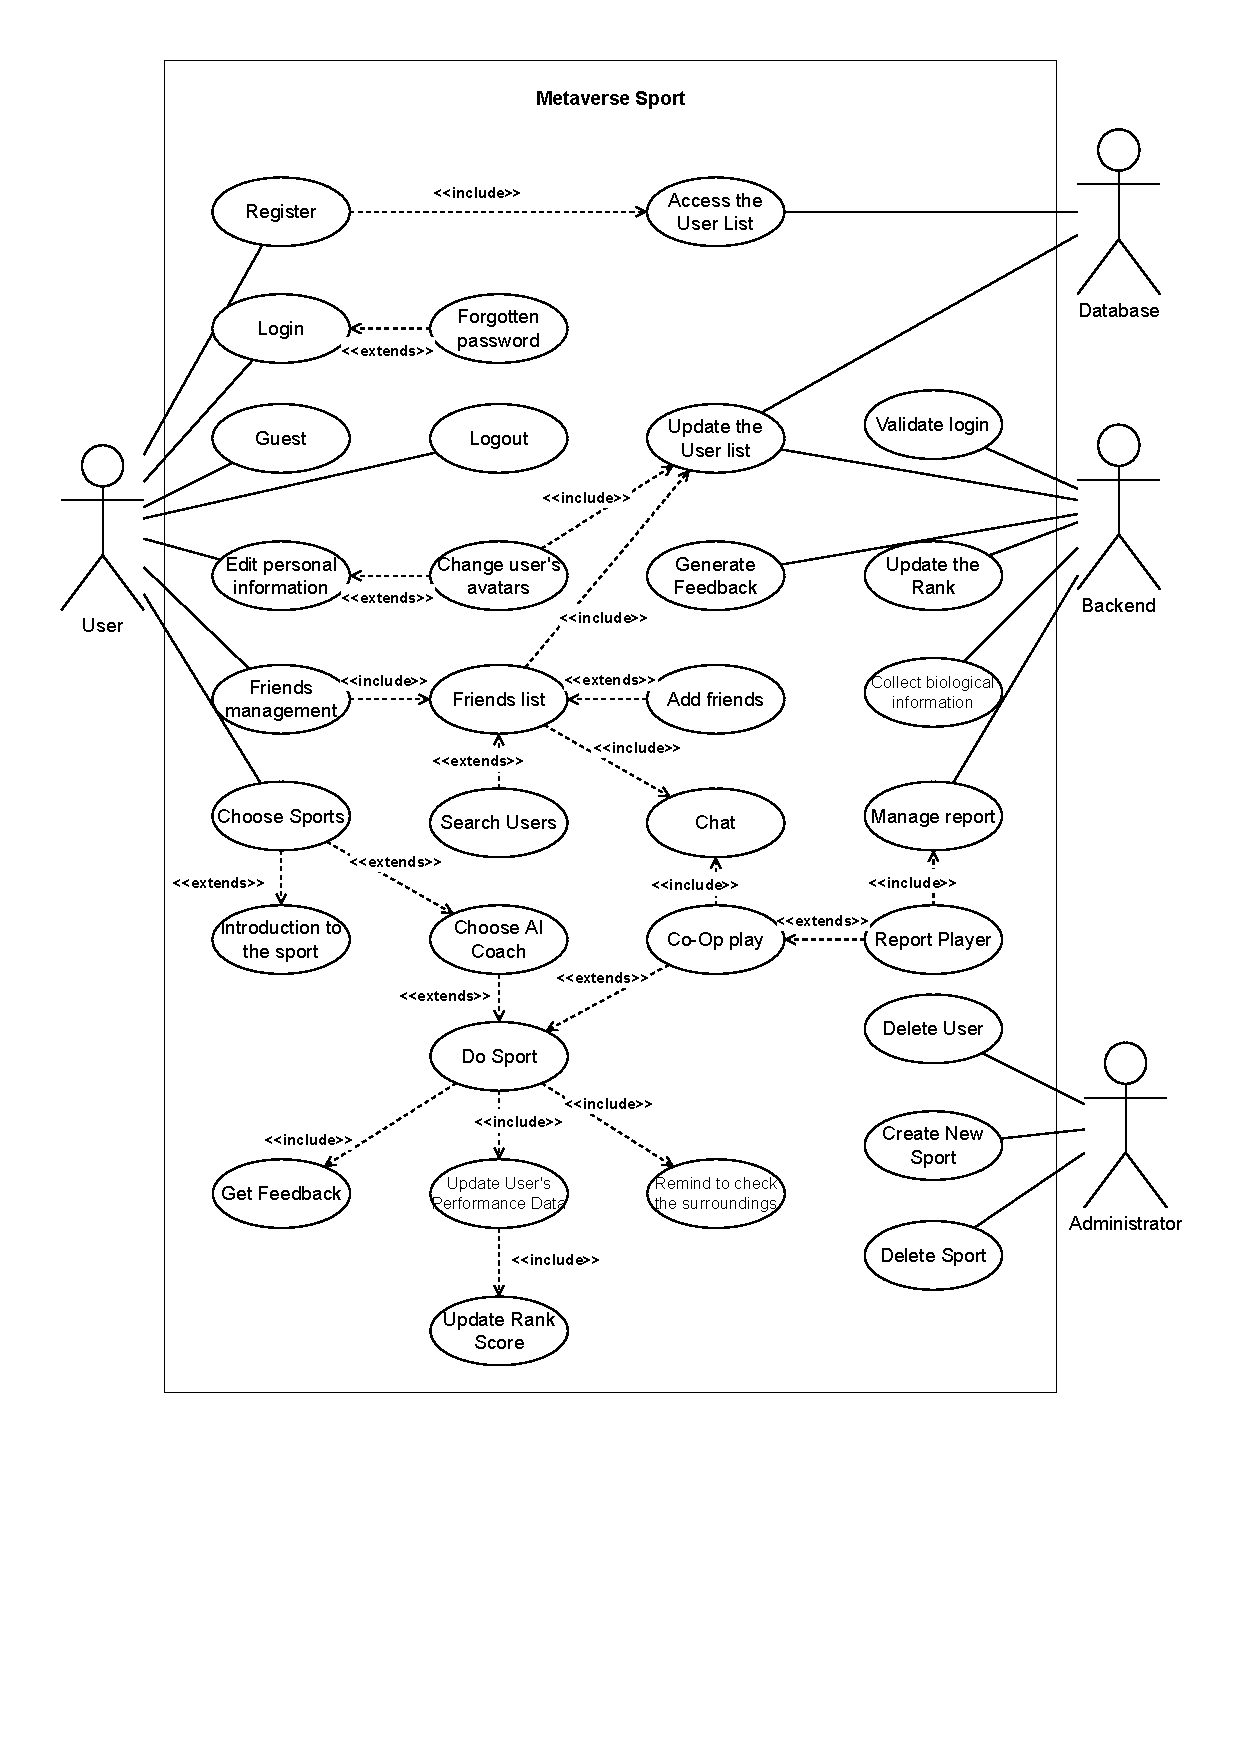
\includegraphics[width=0.95\textwidth]{images/UseCaseDiagram.pdf}
		\label{lable}
	\end{figure}
	\newpage

	\subsection{Use Case Specification \& Scenarios}

	\noindent{\Large\textbf{Use Case1: Login \& Register}}

	\begin{itemize}
		\item[] \textbf{Actors:}
		\begin{quote}
			User, Backend
		\end{quote}
		\item[] \textbf{Precondtion:}
		\begin{enumerate}[itemindent=1em]
			\item System allows the user to select the `Guest' option in the event that they are not ready to register yet.
			\item System displays current users that already exist.				
		\end{enumerate}
		\item[] \textbf{Flow of Events:}
		\begin{enumerate}[itemindent=1em]
			\item User enters an email.
			\item Backend checks for validity of the email.
			\item User enters a password.
			\item Backend checks that the password meets the requirements of what would be considered a “good password”.
			\item User enters date of birth.
			\item Backend checks that the user meets the age requirement.
			\item User enters a username.
			\item User enters a mobile phone number (optional).
			\item User consents to the Terms of Service.
			\item User consents to the collection of their biological information (optional).
			\item User clicks the “Create Account” button.
			\item Backend sends a verification email and a code to the mobile phone number (if one was provided).
			\item User verifies email and mobile phone number.					
		\end{enumerate}
		\item[] \textbf{Postcondtion:}
		\begin{enumerate}[itemindent=1em]
			\item User account is created.
			\item Backend updates the system and database with the new account and the user is given the option to login with their username/email (either is fine) and password.			
		\end{enumerate}
		\item[] \textbf{Scenario 1:}
		\par \hspace*{1cm} Sheldon is interested in learning new types of sports that he has never played before and exploring the use of guided training with an AI coach to improve his existing sports skills. He was recommended an application called Metaverse Augmented Reality Sports by his friends and he then downloaded the application on his device. Upon opening the application, he is asked to log in as an existing user or sign up. Since he is new to the application, he has chosen to register for an account. The first step of registration requires him to enter an email address, followed by an email verification which involves the system checking whether the given email address is valid and/or already being used. Once this step is completed, he is required to create a unique password according to the criteria specified by the application. Following this step, he is then required to introduce his date of birth and enter a valid username, and is given the option to enter his mobile phone number for further account security and protection. He is then required to accept the Terms, Privacy Policy and Conditions, and he is also given options to enter his biological information for a better user experience. After clicking “Create Account”, the last step requires him to validate his email address by clicking on a link sent to his email. Once this is completed, his account is now created.
		\item[] \textbf{Scenario 2:}
		\par \hspace*{1cm} Eren would like to register an account for the application Metaverse Augmented Reality Sports after hearing that it would help him improve his sports skills. As he does not initially have an account, he chooses to register for one, and he enters his email, which the system verifies to be valid. However, upon entering a password, a message appears saying that the password is too weak. Eren realises that he must change the password, and so he adds in some special characters to make it strong, and the system accepts it. After doing so, he enters his date of birth, enters a username, enters his phone number, and accepts the Terms, Privacy Policy and Conditions, but he decides not to enter his biological information. He then clicks “Create Account”, verifies his email via a link sent to his email, and his phone number via a code sent to his phone, and successfully creates his account.
	\end{itemize}

	\hspace*{\fill}\\
	\noindent{\Large\textbf{Use Case2: Do Sport - AI Coach}}

	\begin{itemize}
		\item[] \textbf{Actors:}
		\begin{quote}
			user, backend, action sensor, Human Health Monitoring System
		\end{quote}
		\item[] \textbf{Precondtion:}
		\begin{enumerate}[itemindent=1em]
			\item Devices are charged and placed correctly
			\item Devices are connected to the network
			\item User is already logged in
			\item There are no obstacles around the user
		\end{enumerate}
		\item[] \textbf{Flow of Events:}
		\begin{enumerate}[itemindent=1em]
			\item User browses the interface to find the desired sport
			\item User selects a sport and coach, and then views the introduction of the sport
			\item User chooses to start exercise course
			\item The backend reminds the user to check for surrounding obstacles
			\item The user checks the surroundings and finds no obstacles, and chooses to continue
			\item The backend starts playing the exercise course
			\item The backend starts to collect the user's body data through the Human Health Monitoring System
			\item The backend reminds the user of action skills during the user's exercise, and performs action analysis through the action sensor
			\item The user has finished the exercise course
			\item The backend stops collecting the user's body data
			\item The backend generates biometric analysis of this training through the data of the Human Health Monitoring System
			\item The backend generates the ranking score created by the exercise course performance
			\item The backend updates the users performance statistics to the ranking list	
		\end{enumerate}
		\item[] \textbf{Postcondtion:}
		\begin{enumerate}[itemindent=1em]
			\item The user do not experience health problems during exercise
			\item Action sensor works normally
			\item The system do not report error during the exercise
			\item The rank score is generated correctly	
		\end{enumerate}
		\item[] \textbf{Scenario 1:}
		\par \hspace*{1cm} Jenny loves to dance but has been unable to attend any dance lessons due to the  COVID-19 pandemic. She discovered the Metaverse Augmented Reality Sports within the Metaverse, which allows her to start practicing the basics at home. Jenny put on the MR device, and turned on the motion sensor and Human Health Monitoring System which were already connected to the Internet. After logging in, Jenny opened the sports interface and began to browse the available sports. She found the dancing course and chose to start. A warning popped up on the interface and asked Jenny to check the surroundings for any potential hazards. Jenny started dancing after confirming that her surroundings were safe. The AI coach advised Jenny to adjust her posture when executing certain moves to help improve her dance skills. After the course was completed, a pop-up window appeared which broke down her performance during the training course and encouraged Jenny to continue practicing. At the same time, Jenny also saw that her rank score increased.
		\item[] \textbf{Scenario 2:}
		\par \hspace*{1cm} Tobias has been playing badminton with his friend and has noticed his friend has considerably improved. Curious, Tobias asks his friend how he improved so drastically; his friend tells him that he has been using the Metaverse Augmented Reality Sports application for advice from the AI Coach based on his performance. He goes home and decides to use his MR device, motion sensor and Human Health Monitoring System to try out this app for himself. Tobias goes directly to the browse sports page and selects badminton, after the environmental safety notification and confirmation, Tobias begins to start his coaching. Tobias receives a pop-up window with feedback he finds valuable and useful, so he decided to begin practicing in conjunction with the AI coach for an hour every day that week. This practice led to him improving his smash and flick techniques. The following week, Tobias had a rematch with his friend in person and was complimented on how much he had improved.
	\end{itemize}

	\hspace*{\fill}\\
	\noindent{\Large\textbf{Use Case3: Adding Friends}}

	\begin{itemize}
		\item[] \textbf{Actors:}
		\begin{quote}
			User1, User2 , backend, Database
		\end{quote}
		\item[] \textbf{Precondtion:}
		\begin{enumerate}[itemindent=1em]
			\item Devices are charged and placed correctly
			\item Devices are connected to the network
			\item User1 and User2 are already logged in
			\item User1 already get the correct User ID of User2
		\end{enumerate}
		\item[] \textbf{Flow of Events:}
		\begin{enumerate}[itemindent=1em]
			\item User1 opens up the friends list / ranking \& score board and the board shows the top 100 players and whether they are currently on line
			\item User1 clicks the button to search a user
			\item User1 enters user ID of user2 in the search bar
			\item The Backend receives the user ID and searches for it in Database
			\item The Database finds user2 and returns the information to the Backend
			\item Backend displays the information of user 2 in the interface
			\item User1 clicks the send friend request button to add a friend
			\item The backend receives the instruction and then sends the request of adding friends to the user2
			\item User2 clicks the button to accept the friend request received from User1
			\item Backend update the friend list of user1 and user2		
		\end{enumerate}
		\item[] \textbf{Postcondtion:}
		\begin{enumerate}[itemindent=1em]
			\item The system don't report error during the friend management
			\item The Database stores the information correctly
		\end{enumerate}
		\item[] \textbf{Scenario 1:}
		\par \hspace*{1cm} Jake and Steve are very good friends. During one of their conversations, they found out that they were both using a popular software, Metaverse Augmented Reality Sports. Steve gave Jake his User ID. Jake put on the MR device after he got home. Jake opened the friends interface and chose to search for ID. After entering Steve's ID, Jake sees Steve's user information and clicks `Add Friend'. On the receiving end, Steve logs in and the system notifies him that someone is requesting to be his friend. After confirming it was from his friend Jake, Steve clicked accept. They are now friends on Metaverse Sport.
		\item[] \textbf{Scenario 2:}
		\par \hspace*{1cm} Adam is learning to play badminton but is still a beginner. He wants to improve his skill more efficiently and would like to meet a player who plays better than him. One day he logged into the Metaverse Sport Application, browsed the ranking \& score board and checked the top 100 players. Adam found George appeared on the rank and decided to make friends with him. So Adam entered George's ID and sent an invitation to ask George to add a friend. At that time, George had just finished his training and was available. Therefore George clicked and accepted the invitation. Now Adam and George are friends on Metaverse Sport Application. 
	\end{itemize}

	\hspace*{\fill}\\
	\noindent{\Large\textbf{Use Case4: Edit Personal Information}}

	\begin{itemize}
		\item[] \textbf{Actors:}
		\begin{quote}
			user, backend
		\end{quote}
		\item[] \textbf{Precondtion:}
		\begin{enumerate}[itemindent=1em]
			\item User is already logged in
			\item The application is connected to the network			
		\end{enumerate}
		\item[] \textbf{Flow of Events:}
		\begin{enumerate}[itemindent=1em]
			\item User views his/her own home page
			\item User clicks `edit profile'
			\item User clicks the avatar
			\item Backend prompts user to change the avatar
			\item User clicks `upload a new avatar' button
			\item Backend prompts user to take a photo or upload from local pictures
			\item 
			a. 1) User selects to take a photo\\
			\hspace*{0.7cm} 2) Backend request for camera and photo access\\
			\hspace*{0.7cm} 3) User clicks `agree' button\\
			\hspace*{0.7cm} 4) User takes a photo\\
			\hspace*{0.7cm} 5) Backend prompts user to edit current photo\\
			\hspace*{0.7cm} 6) User changes the size of photo\\
			\hspace*{0.7cm} 7) User adds a filter to the photo\\
			\hspace*{0.7cm} 8) User clicks `finish' button\\
			\hspace*{0.25cm} b. 1)  User selects to upload from local pictures\\
    		\hspace*{0.7cm} 2)  Backend prompts user to browse and choose the location\\
    		\hspace*{0.7cm} 3)  User selects a documentary and clicks a photo file\\
    		\hspace*{0.7cm} 4)  User clicks `confirm' button
			\item User clicks `upload' button
			\item Backend changes the avatar
			\item User clicks `username' button
			\item Backend prompts user to input a new username
			\item User inputs a new username
			\item User clicks `save' button
			\item Backend changes user's username
			\item User clicks `introduction' button
			\item Backend prompts user to input a new introduction
			\item User inputs a new introduction
			\item User clicks `save' button
			\item Backend changes user's introduction
		\end{enumerate}
		\item[] \textbf{Postcondtion:}
		\begin{enumerate}[itemindent=1em]
			\item User's avatar has been updated successfully
			\item User's username has been updated successfully
			\item User's introduction has been updated successfully			
		\end{enumerate}
		\item[] \textbf{Scenario 1:}
		\par \hspace*{1cm} Fannie has a beautiful selfie and she want to use it as her avatar in the AI Sport application. Fannie login in the app and click the personal information button. Then She clicks the old avatar and chooses the editor function. After that she chooses her favorite picture on her phone and clicks the confirm button, so now she has a beautiful avatar in this application. In addition, she design an interesting username in order to make herself more attractive in the friends cycle in this application. Therefore she click the old username and modify it as new username. Besides, Fannie click the introduction button and edit her introduction, then save it. Congratulatively, now Fannie has new avatar, username and introduction.
		\item[] \textbf{Scenario 2:}
		\par \hspace*{1cm} Martha wants to change her avatar in the AI Sport application. She signs in the system and goes to her profile page. Then she clicks the `edit profile' button and clicks her avatar. She chooses to upload a new avatar and picks one beautiful picture from a local folder. After that she clicks the `confirm' button but the system indicates that the file uploaded does not meet the requirements because the size of the file should not exceed 2M. So unfortunately Martha fails to change her avatar. Then Martha wants to change her username and she clicks the `username' button and inputs `martha<>', but the system prompts that it is not a valid name because it contains invalid characters. So unfortunately Martha fails to save a new username.
	\end{itemize}

	\subsection{Activity Diagram}

	\begin{figure}[H]
		\centering
		\caption*{\textbf{Diagram2.2} Report a suspicious user}
		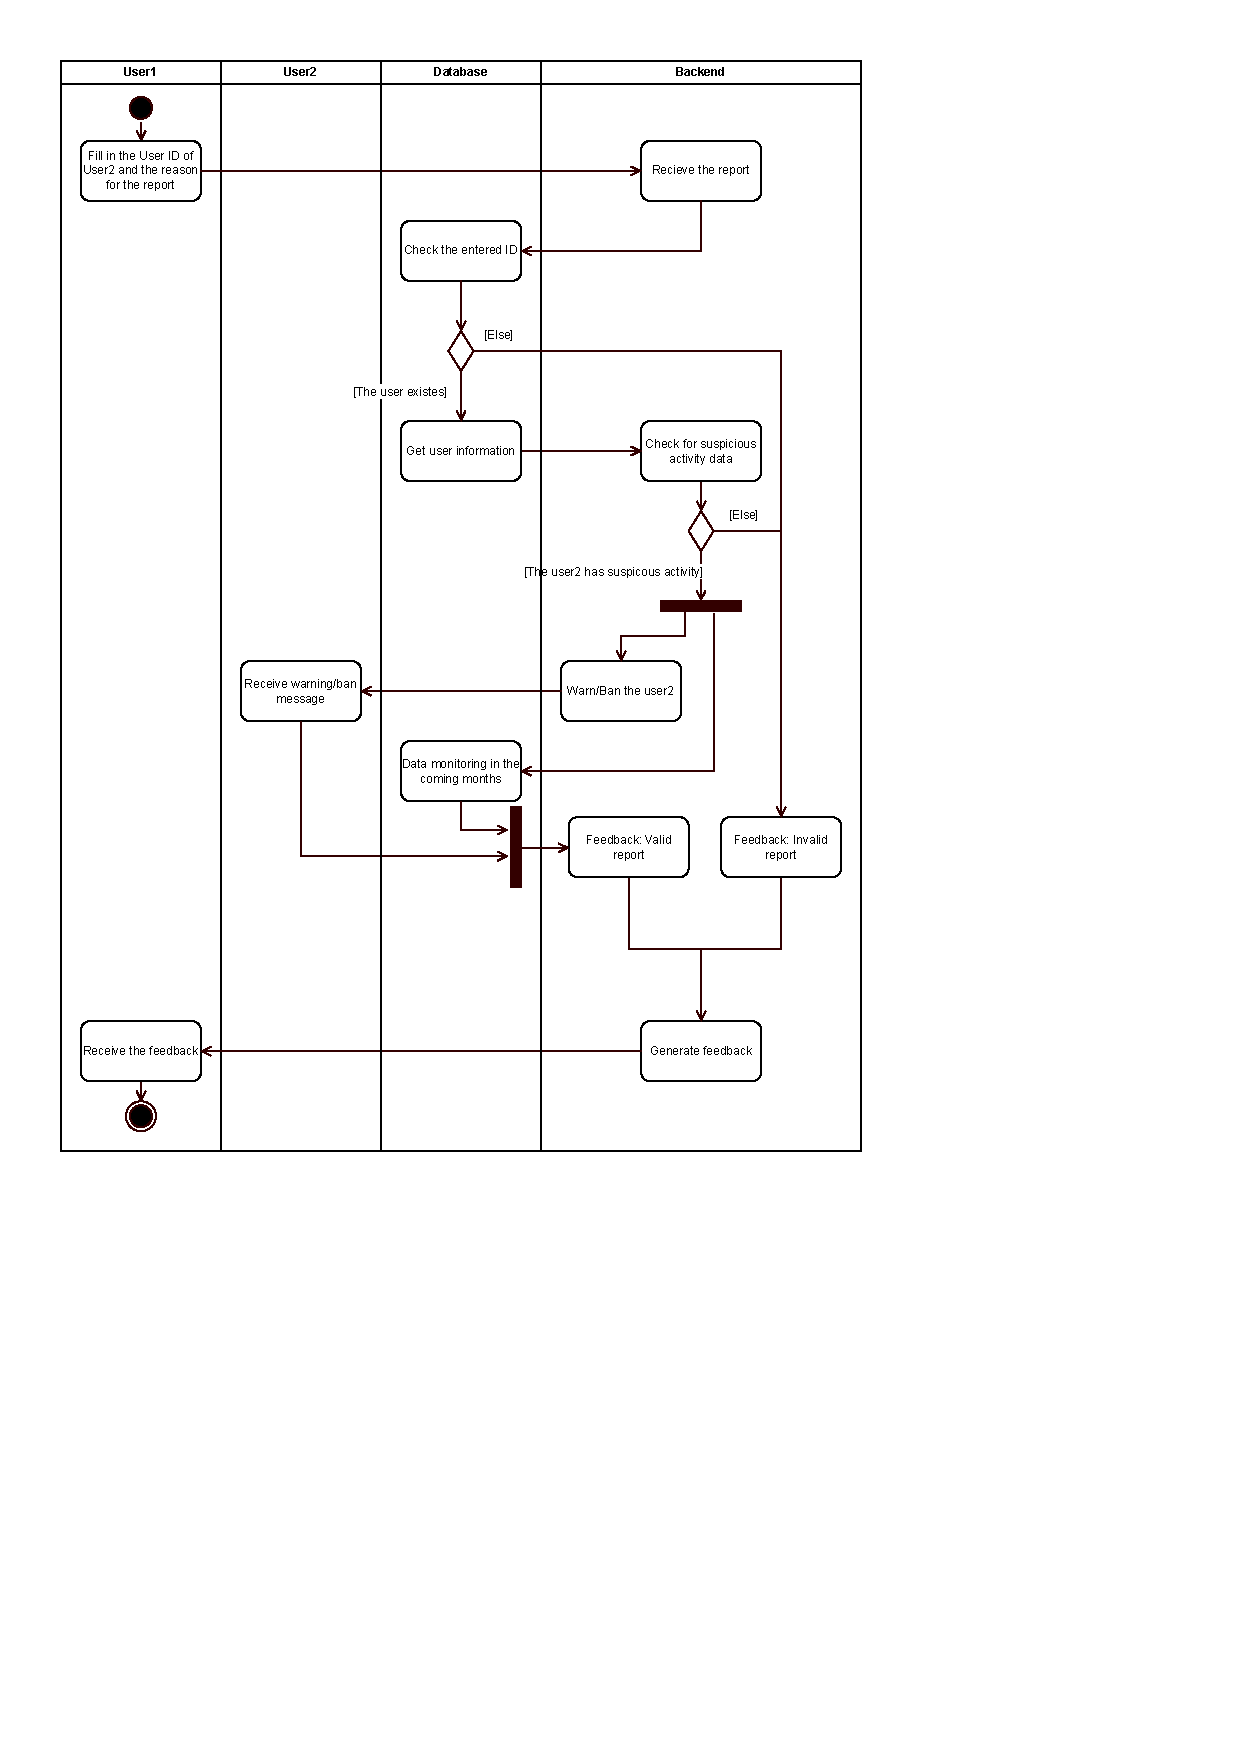
\includegraphics[width=\textwidth]{images/ActivityDiagram_Report.pdf}
		\label{AD_Report}
	\end{figure}
	\newpage

	\begin{figure}[H]
		\centering
		\caption*{\textbf{Diagram2.3} Co-Op sport with friend}
		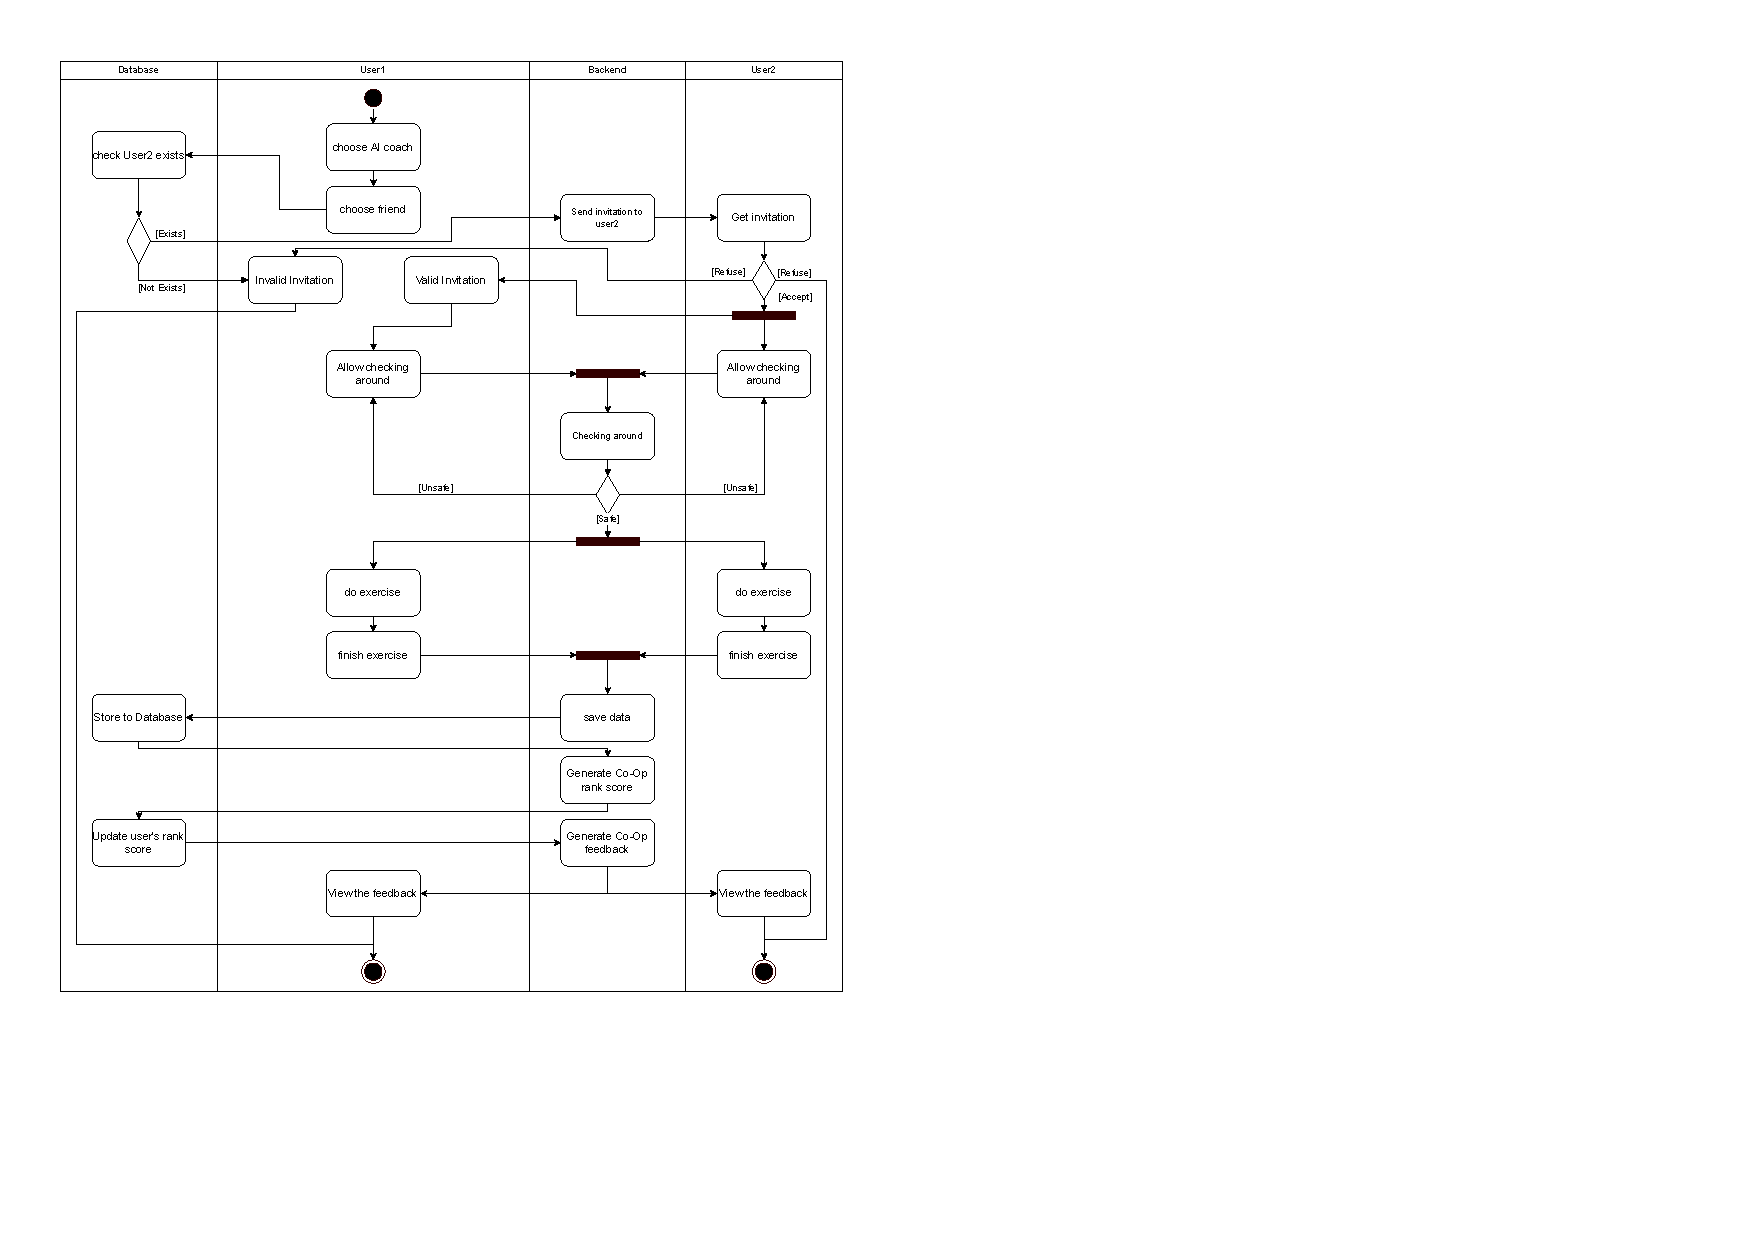
\includegraphics[width=\textwidth]{images/ActivityDiagram_CoOp.pdf}
		\label{AD_CoOp}
	\end{figure}
	\newpage

	\subsection{Class Analysis}

	\subsubsection{Noun-verb Analysis}

	\begin{table}[h!]
		\caption*{\textbf{Diagram2.4} Noun Analysis}
		\noindent\begin{minipage}{\textwidth}
			\begin{minipage}[t]{0.48\textwidth}
		 	\centering
			\makeatletter\def\@captype{table}\makeatother
			  	\begin{tabular}{|p{0.7\linewidth}|p{0.2\linewidth}|} 
		   			\hline
					\textbf{Noun words} & \textbf{Used} \\
					\hline
					Avatar & Yes\\
					\hline
					Avatar frame & Yes\\
					\hline
					action sensor & Yes\\
					\hline
					age & Yes\\
					\hline
					AI coach & Yes\\
					\hline
					Chat & Yes\\
					\hline
					Database & Yes\\
					\hline
					Date & \\
					\hline
					device & Yes\\
					\hline
					feedback & Yes\\
					\hline
					FPS & Yes\\
					\hline
					Friend management & Yes\\
					\hline
					Friends list & Yes\\
					\hline
					Gender & Yes\\
					\hline
					health monitoring system & Yes\\
					\hline
		   		\end{tabular}
		 	\end{minipage}
		 	\begin{minipage}[t]{0.48\textwidth}
		  	\centering
			   	\makeatletter\def\@captype{table}\makeatother
				\begin{tabular}{|p{0.7\linewidth}|p{0.2\linewidth}|}        
					\hline
					\textbf{Noun words} & \textbf{Used} \\
					\hline
					heart rate& Yes\\
					\hline
					history & Yes\\
					\hline
					ID & Yes\\
					\hline
					interaction & \\
					\hline
					Introduction & Yes\\
					\hline
					Language & Yes\\
					\hline
					Message & Yes\\
					\hline
					password & Yes\\
					\hline
					personal information &Yes\\
					\hline
					rank & Yes\\
					\hline
					rank points & Yes\\
					\hline
					Social Setting & Yes\\
					\hline
					Sports & Yes\\
					\hline
					types & \\
					\hline
					User & Yes\\
					\hline
			 	\end{tabular}
		  	\end{minipage}
   		\end{minipage}
	\end{table}

	\begin{table}[h!]
		\caption*{\textbf{Diagram2.5} Verb Analysis}
		\noindent\begin{minipage}{\textwidth}
			\begin{minipage}[t]{0.48\textwidth}
		 	\centering
			\makeatletter\def\@captype{table}\makeatother
			  	\begin{tabular}{|p{0.7\linewidth}|p{0.2\linewidth}|} 
		   			\hline
					\textbf{Noun words} & \textbf{Used} \\
					\hline
					Accept invites & Yes\\
					\hline
					Accessing coach & \\
					\hline
					Add friends & Yes\\
					\hline
					Analyze sports data & Yes\\
					\hline
					Browse coach & Yes\\
					\hline
					Browse sports & Yes\\
					\hline
					Charge devices & \\
					\hline
					Chat with friends & Yes\\
					\hline
					Choose sports/coach/friends& Yes\\
					\hline
					Collect points & Yes\\
					\hline
					confirm environment safety & Yes\\
					\hline
					Connected sensor device & Yes\\
					\hline
					Customize avatar & Yes\\
					\hline
					Detect devices & Yes\\
					\hline
					Edit/Create profile information& Yes\\
					\hline
					enable subtitiles& Yes\\
					\hline
		   		\end{tabular}
		 	\end{minipage}
		 	\begin{minipage}[t]{0.48\textwidth}
		  	\centering
			   	\makeatletter\def\@captype{table}\makeatother
				\begin{tabular}{|p{0.7\linewidth}|p{0.2\linewidth}|}        
					\hline
					\textbf{Noun words} & \textbf{Used} \\
					\hline
					Forget password & Yes\\
					\hline
					Generates feedback & Yes\\
					\hline
					Log in & Yes\\
					\hline
					Pause the course & Yes\\
					\hline
					Play sports & Yes\\
					\hline
					Receive feedback & Yes\\
					\hline
					Register & Yes\\
					\hline
					Save data & Yes\\
					\hline
					Search for a new friend & Yes\\
					\hline
					set volume & Yes\\
					\hline
					Skip parts of the course & Yes\\
					\hline
					Stops course & Yes\\
					\hline
					submit user's sports data & Yes\\
					\hline
					Update changes to friend list & Yes\\
					\hline
					Verify email & \\
					\hline
					View the feedback history & Yes\\
					\hline
			 	\end{tabular}
		  	\end{minipage}
   		\end{minipage}
	\end{table}

	\subsubsection{CRC Cards}
	
	\noindent\begin{minipage}{\textwidth}
		\begin{minipage}[t]{0.48\textwidth}
	 	\centering
		\makeatletter\def\@captype{table}\makeatother\caption*{}
		  	\begin{tabular}{|p{0.44\linewidth}|p{0.44\linewidth}|} 
	   			\hline
				\multicolumn{2}{|c|}{\textbf{Class Name}} \\
				\hline
				\multicolumn{2}{|c|}{User Account} \\
				\hline
				\textbf{Responsibility} & \textbf{Collaborator} \\
				\hline
				LogIn & Sport\\
				LogOut & Setting Options\\
				Register & Friend Management\\
				ForgetPassword & \\
				& \\
				& \\
				& \\
				\hline
	   		\end{tabular}
	 	\end{minipage}
	 	\begin{minipage}[t]{0.48\textwidth}
		\centering
		\makeatletter\def\@captype{table}\makeatother\caption*{}
			\begin{tabular}{|p{0.48\linewidth}|p{0.40\linewidth}|} 
				\hline
				\multicolumn{2}{|c|}{\textbf{Class Name}} \\
				\hline
				\multicolumn{2}{|c|}{Sport} \\
				\hline
				\textbf{Responsibility} & \textbf{Collaborator} \\
				\hline
				BrowseSport & User Account\\
				ChooseSport & AI Coach \\
				PlaySport & Device \\
				PauseCourse & Rank \\
				StopCourse & \\
				SkipPart & \\
				ViewWorkoutRecords& \\
				\hline
			\end{tabular}
		\end{minipage}
	\end{minipage}

	\noindent\begin{minipage}{\textwidth}
		\begin{minipage}[t]{0.48\textwidth}
	 	\centering
		\makeatletter\def\@captype{table}\makeatother\caption*{}
		  	\begin{tabular}{|p{0.48\linewidth}|p{0.40\linewidth}|} 
	   			\hline
				\multicolumn{2}{|c|}{\textbf{Class Name}} \\
				\hline
				\multicolumn{2}{|c|}{AI Coach} \\
				\hline
				\textbf{Responsibility} & \textbf{Collaborator} \\
				\hline
				BrowseCoach & Sport\\
				ChooseCoach & Feedback \\
				AnalyseData &  \\
				\hline
	   		\end{tabular}
	 	\end{minipage}
	 	\begin{minipage}[t]{0.48\textwidth}
		\centering
		\makeatletter\def\@captype{table}\makeatother\caption*{}
			\begin{tabular}{|p{0.48\linewidth}|p{0.40\linewidth}|} 
				\hline
				\multicolumn{2}{|c|}{\textbf{Class Name}} \\
				\hline
				\multicolumn{2}{|c|}{Feedback} \\
				\hline
				\textbf{Responsibility} & \textbf{Collaborator} \\
				\hline
				GeneratesFeedback & AI Coach \\
				SendFeedback & Rank\\
				StoreFeedback & \\
				\hline
			\end{tabular}
		\end{minipage}
   	\end{minipage}

	\noindent\begin{minipage}{\textwidth}
		\begin{minipage}[t]{0.48\textwidth}
	 	\centering
		\makeatletter\def\@captype{table}\makeatother\caption*{}
		  	\begin{tabular}{|p{0.48\linewidth}|p{0.40\linewidth}|} 
	   			\hline
				\multicolumn{2}{|c|}{\textbf{Class Name}} \\
				\hline
				\multicolumn{2}{|c|}{Rank} \\
				\hline
				\textbf{Responsibility} & \textbf{Collaborator} \\
				\hline
				GeneratesRankPoints & AI Coach\\
				CollectPoints & Sport\\
				UpdateRank & \\
				\hline
	   		\end{tabular}
	 	\end{minipage}
	 	\begin{minipage}[t]{0.48\textwidth}
		\centering
		\makeatletter\def\@captype{table}\makeatother\caption*{}
			\begin{tabular}{|p{0.48\linewidth}|p{0.40\linewidth}|} 
				\hline
				\multicolumn{2}{|c|}{\textbf{Class Name}} \\
				\hline
				\multicolumn{2}{|c|}{Device} \\
				\hline
				\textbf{Responsibility} & \textbf{Collaborator} \\
				\hline
				CheckDevice & User\\
				ConnectDevice & Sensor\\
				DeviceUpdate & HealthMonitor\\
				\hline
			\end{tabular}
		\end{minipage}
   	\end{minipage}

	\noindent\begin{minipage}{\textwidth}
		\begin{minipage}[t]{0.48\textwidth}
		\centering
		\makeatletter\def\@captype{table}\makeatother\caption*{}
			\begin{tabular}{|p{0.40\linewidth}|p{0.48\linewidth}|} 
				\hline
				\multicolumn{2}{|c|}{\textbf{Class Name}} \\
				\hline
				\multicolumn{2}{|c|}{Friend Management} \\
				\hline
				\textbf{Responsibility} & \textbf{Collaborator} \\
				\hline
				OpenFriendList& User Account\\
				StartChat & Friend List\\
				& Chat\\
				\hline
			\end{tabular}
		\end{minipage}
	 	\begin{minipage}[t]{0.48\textwidth}
		\centering
		\makeatletter\def\@captype{table}\makeatother\caption*{}
			\begin{tabular}{|p{0.44\linewidth}|p{0.44\linewidth}|} 
				\hline
				\multicolumn{2}{|c|}{\textbf{Class Name}} \\
				\hline
				\multicolumn{2}{|c|}{Sensor} \\
				\hline
				\textbf{Responsibility} & \textbf{Collaborator} \\
				\hline
				CollectSensorData & Device \\
				UploadSensorData & Action Sensor\\
				TurnOnSensor & Environment Sensor\\
				\hline
			\end{tabular}
		\end{minipage}
   	\end{minipage}

	\noindent\begin{minipage}{\textwidth}
		\begin{minipage}[t]{0.48\textwidth}
	 	\centering
		\makeatletter\def\@captype{table}\makeatother\caption*{}
		  	\begin{tabular}{|p{0.48\linewidth}|p{0.40\linewidth}|} 
	   			\hline
				\multicolumn{2}{|c|}{\textbf{Class Name}} \\
				\hline
				\multicolumn{2}{|c|}{Action Sensor} \\
				\hline
				\textbf{Responsibility} & \textbf{Collaborator} \\
				\hline
				ActionComparation & Sensor\\
				\hline
	   		\end{tabular}
	 	\end{minipage}
	 	\begin{minipage}[t]{0.48\textwidth}
		\centering
		\makeatletter\def\@captype{table}\makeatother\caption*{}
			\begin{tabular}{|p{0.52\linewidth}|p{0.36\linewidth}|} 
				\hline
				\multicolumn{2}{|c|}{\textbf{Class Name}} \\
				\hline
				\multicolumn{2}{|c|}{Environment Sensor} \\
				\hline
				\textbf{Responsibility} & \textbf{Collaborator} \\
				\hline
				CheckEnvironmentSafety& Sensor\\
				\hline
			\end{tabular}
		\end{minipage}
   	\end{minipage}

	\noindent\begin{minipage}{\textwidth}
		\begin{minipage}[t]{0.48\textwidth}
		\centering
		\makeatletter\def\@captype{table}\makeatother\caption*{}
			\begin{tabular}{|p{0.48\linewidth}|p{0.40\linewidth}|} 
				\hline
				\multicolumn{2}{|c|}{\textbf{Class Name}} \\
				\hline
				\multicolumn{2}{|c|}{HealthMonitor} \\
				\hline
				\textbf{Responsibility} & \textbf{Collaborator} \\
				\hline
				TurnOnHealthMonitor & Device\\
				UpdateHealthData & \\
				GiveWarning & \\
				CallEmergency &\\
				\hline
			\end{tabular}
		\end{minipage}
		\begin{minipage}[t]{0.48\textwidth}
		\centering
		\makeatletter\def\@captype{table}\makeatother\caption*{}
			\begin{tabular}{|p{0.40\linewidth}|p{0.48\linewidth}|} 
				\hline
				\multicolumn{2}{|c|}{\textbf{Class Name}} \\
				\hline
				\multicolumn{2}{|c|}{Chat} \\
				\hline
				\textbf{Responsibility} & \textbf{Collaborator} \\
				\hline
				SentMess& Friend Management\\
				ReceiveMess& \\
				DeleteMess& \\
				BrowseChatHistory &\\
				\hline
			\end{tabular}
		\end{minipage}
   	\end{minipage}

	\noindent\begin{minipage}{\textwidth}
		\begin{minipage}[t]{0.48\textwidth}
	 	\centering
		\makeatletter\def\@captype{table}\makeatother\caption*{}
		  	\begin{tabular}{|p{0.40\linewidth}|p{0.48\linewidth}|} 
	   			\hline
				\multicolumn{2}{|c|}{\textbf{Class Name}} \\
				\hline
				\multicolumn{2}{|c|}{Friend List} \\
				\hline
				\textbf{Responsibility} & \textbf{Collaborator} \\
				\hline
				AddFriend & Friend Management\\
				DeleteFriend & Friend\\
				AcceptInvitation & \\
				DeclineInvitation & \\
				UpdateToFL&\\
				\hline
	   		\end{tabular}
	 	\end{minipage}
	 	\begin{minipage}[t]{0.48\textwidth}
		\centering
		\makeatletter\def\@captype{table}\makeatother\caption*{}
			\begin{tabular}{|p{0.40\linewidth}|p{0.48\linewidth}|} 
				\hline
				   \multicolumn{2}{|c|}{\textbf{Class Name}} \\
				   \hline
				   \multicolumn{2}{|c|}{Setting Options} \\
				   \hline
				   \textbf{Responsibility} & \textbf{Collaborator} \\
				   \hline
				   EditOption & User Account\\
				   UpdateToDatabase & User Settings\\
				   &Social Settings\\
				   &General Settings\\
				   &Media Settings\\
				   \hline
			\end{tabular}
		\end{minipage}
   	\end{minipage}

	\noindent\begin{minipage}{\textwidth}
	 	\begin{minipage}[t]{0.48\textwidth}
		\centering
		\makeatletter\def\@captype{table}\makeatother\caption*{}
			\begin{tabular}{|p{0.48\linewidth}|p{0.40\linewidth}|} 
				\hline
				\multicolumn{2}{|c|}{\textbf{Class Name}} \\
				\hline
				\multicolumn{2}{|c|}{Media Settings} \\
				\hline
				\textbf{Responsibility} & \textbf{Collaborator} \\
				\hline
				SetResolution & Setting Options\\
				SetFPS &  \\
				SetVolume & \\
				\hline
			\end{tabular}
		\end{minipage}
		\begin{minipage}[t]{0.48\textwidth}
		\centering
		\makeatletter\def\@captype{table}\makeatother\caption*{}
			\begin{tabular}{|p{0.48\linewidth}|p{0.40\linewidth}|} 
				\hline
				\multicolumn{2}{|c|}{\textbf{Class Name}} \\
				\hline
				\multicolumn{2}{|c|}{Social Setting} \\
				\hline
				\textbf{Responsibility} & \textbf{Collaborator} \\
				\hline
				TurnOffChat & Personal Info\\
				& Setting Options\\
				& Avatar\\
				\hline
			\end{tabular}
		\end{minipage}
   	\end{minipage}

	\noindent\begin{minipage}{\textwidth}
		\begin{minipage}[t]{0.48\textwidth}
	 	\centering
		\makeatletter\def\@captype{table}\makeatother\caption*{}
		  	\begin{tabular}{|p{0.48\linewidth}|p{0.40\linewidth}|} 
	   			\hline
				\multicolumn{2}{|c|}{\textbf{Class Name}} \\
				\hline
				\multicolumn{2}{|c|}{User Setting} \\
				\hline
				\textbf{Responsibility} & \textbf{Collaborator} \\
				\hline
				DeleteAccount& Setting Options\\
				& Personal Info\\
				\hline
	   		\end{tabular}
	 	\end{minipage}
	 	\begin{minipage}[t]{0.48\textwidth}
		\centering
		\makeatletter\def\@captype{table}\makeatother\caption*{}
			\begin{tabular}{|p{0.40\linewidth}|p{0.48\linewidth}|} 
				\hline
				\multicolumn{2}{|c|}{\textbf{Class Name}} \\
				\hline
				\multicolumn{2}{|c|}{Friend} \\
				\hline
				\textbf{Responsibility} & \textbf{Collaborator} \\
				\hline
				Report & Friend List\\
				EditContact & Chat\\
				\hline
			\end{tabular}
		\end{minipage}
   	\end{minipage}

	\noindent\begin{minipage}{\textwidth}
		\begin{minipage}[t]{0.48\textwidth}
	 	\centering
		\makeatletter\def\@captype{table}\makeatother\caption*{}
		  	\begin{tabular}{|p{0.48\linewidth}|p{0.40\linewidth}|} 
	   			\hline
				\multicolumn{2}{|c|}{\textbf{Class Name}} \\
				\hline
				\multicolumn{2}{|c|}{Avatar} \\
				\hline
				\textbf{Responsibility} & \textbf{Collaborator} \\
				\hline
				ChooseAvatar& Social Settings\\
				UploadAvatar& \\
				StoreAvatar& \\
				customiseAvatar& \\
				\hline
	   		\end{tabular}
	 	\end{minipage}
	 	\begin{minipage}[t]{0.48\textwidth}
		\centering
		\makeatletter\def\@captype{table}\makeatother\caption*{}
			\begin{tabular}{|p{0.48\linewidth}|p{0.40\linewidth}|} 
				\hline
				\multicolumn{2}{|c|}{\textbf{Class Name}} \\
				\hline
				\multicolumn{2}{|c|}{Personal Info} \\
				\hline
				\textbf{Responsibility} & \textbf{Collaborator} \\
				\hline
				EditInfo& User Setting\\
				UpdateToDB& Social Setting\\
				DeleteInfo&\\
				BrowseInfo&\\
				\hline
			\end{tabular}
		\end{minipage}
   	\end{minipage}

	\newpage

	\subsubsection{First-Cut Class Diagram}

	\begin{figure}[H]
		\centering
		\caption*{\textbf{Diagram2.6} First-Cut Class Diagram}
		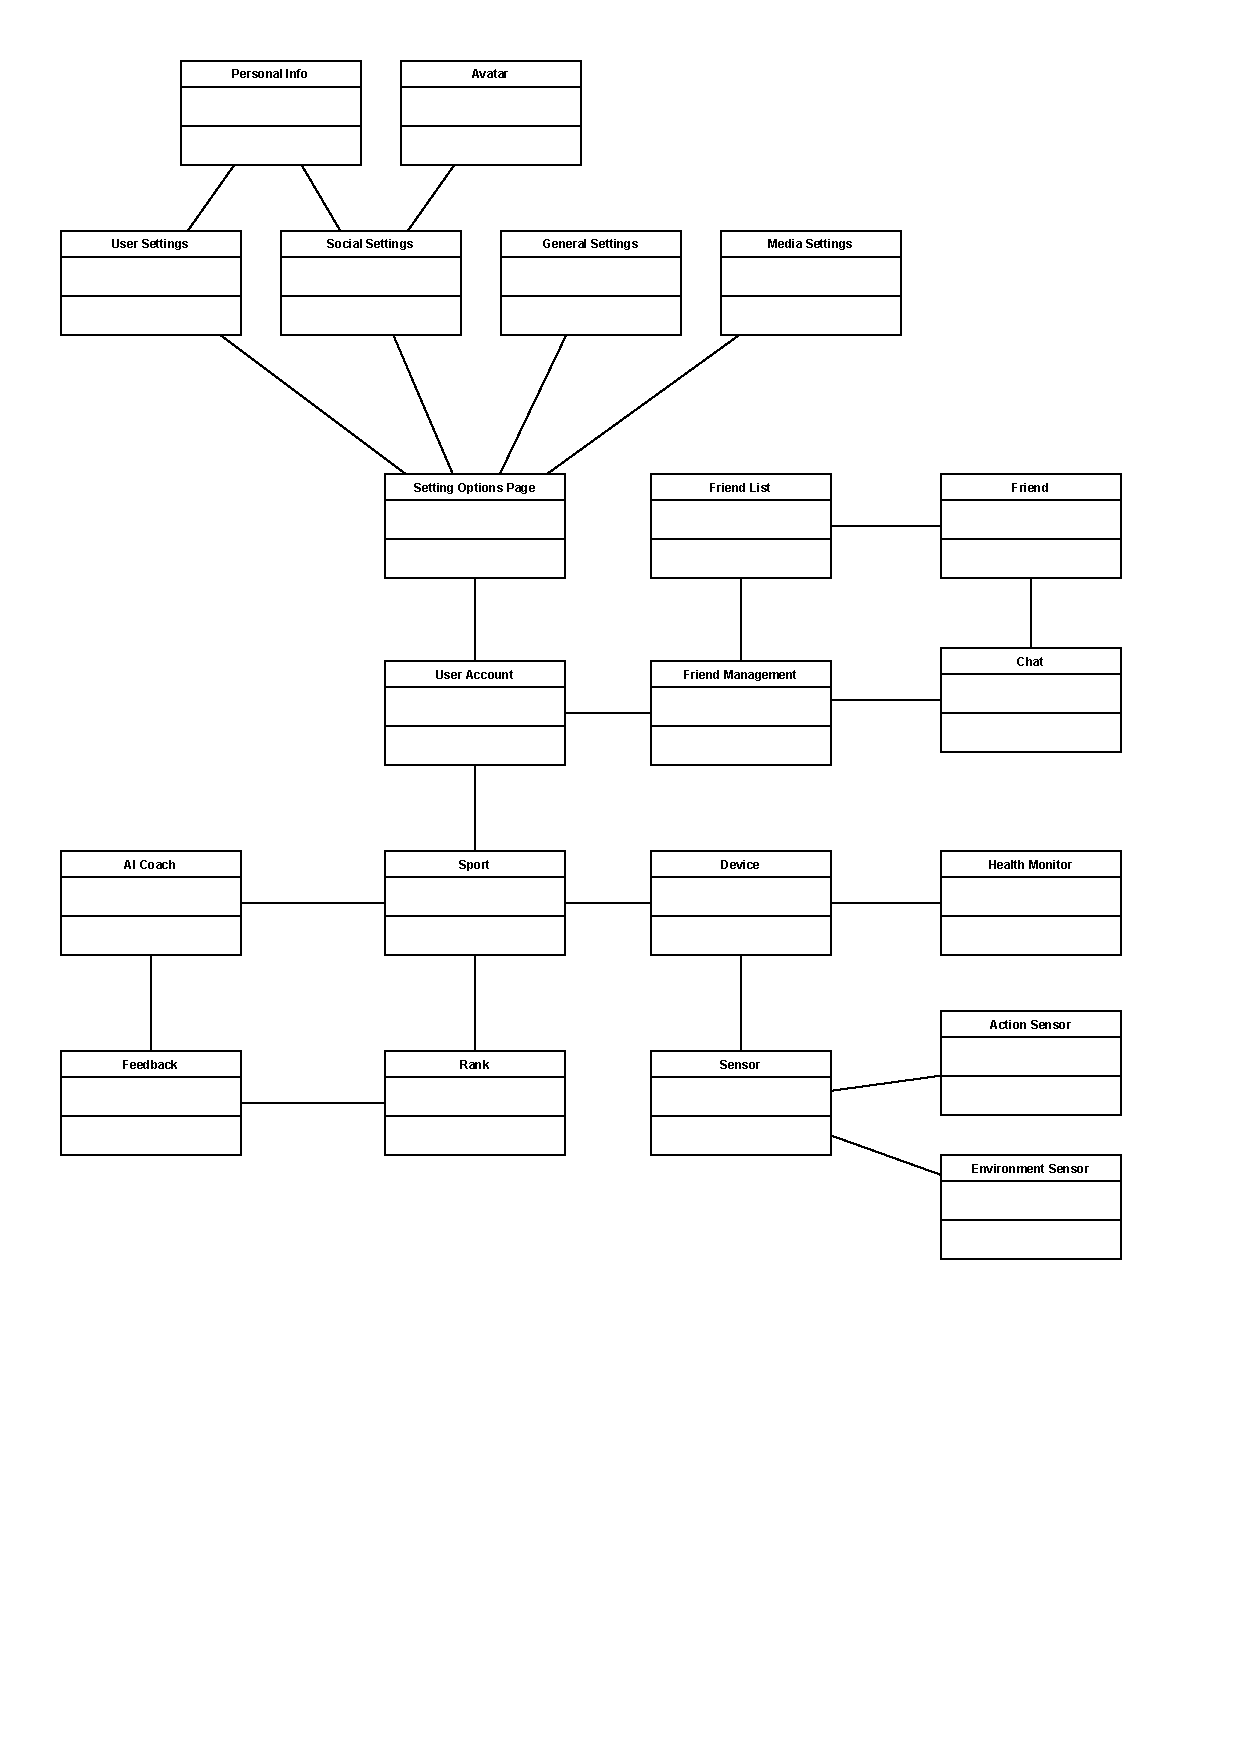
\includegraphics[width = 0.98\textwidth]{images/ClassDiagram_FirstCut.pdf}
		\label{CD_FC}
	\end{figure}

	\subsubsection{Class Diagram}

	\begin{figure}[H]
		\centering
		\caption*{\textbf{Diagram2.7} Class Diagram}
		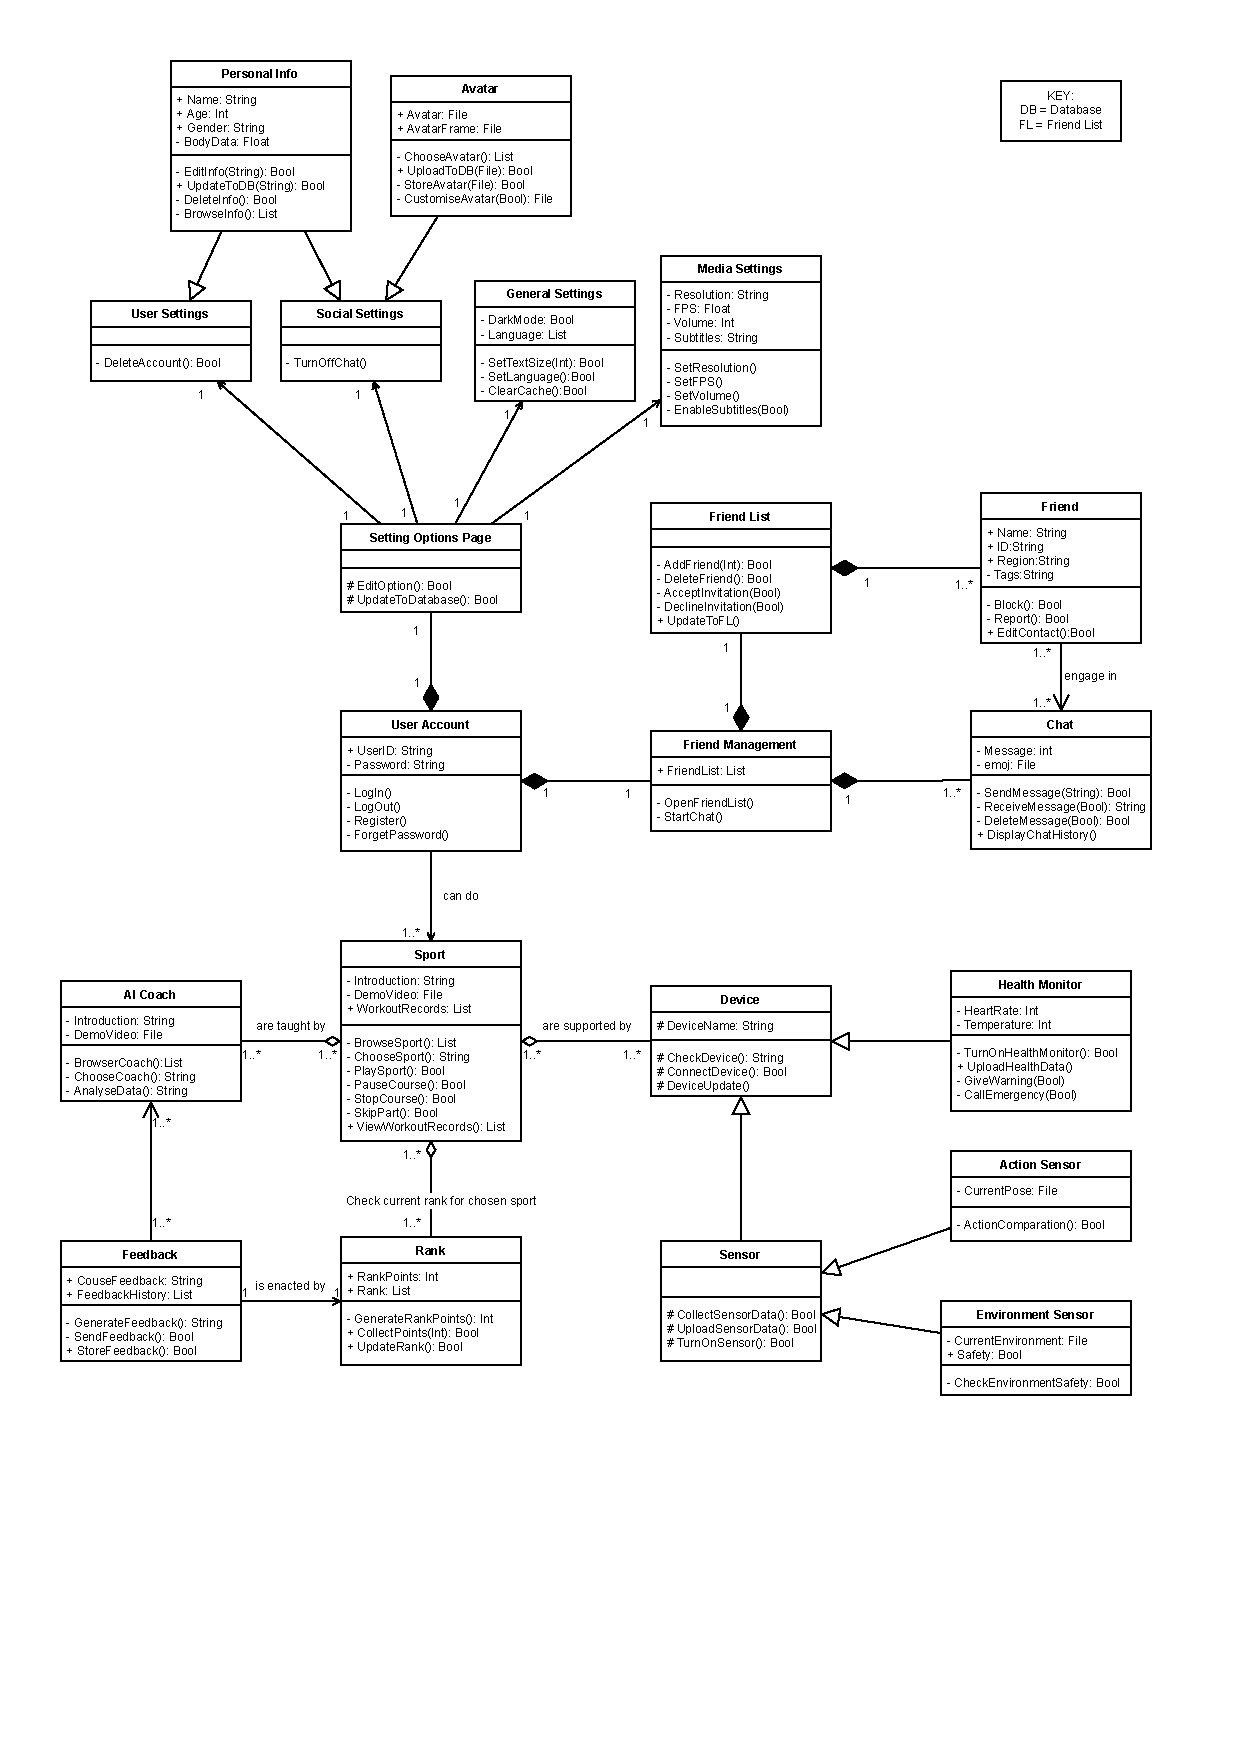
\includegraphics[width=0.95\textwidth]{images/ClassDiagram.pdf}
		\label{CD}
	\end{figure}
	\newpage

	\subsection{Object Diagram}

	\begin{figure}[H]
		\centering
		\caption*{\textbf{Diagram2.8} Object Diagram - Doing sports}
		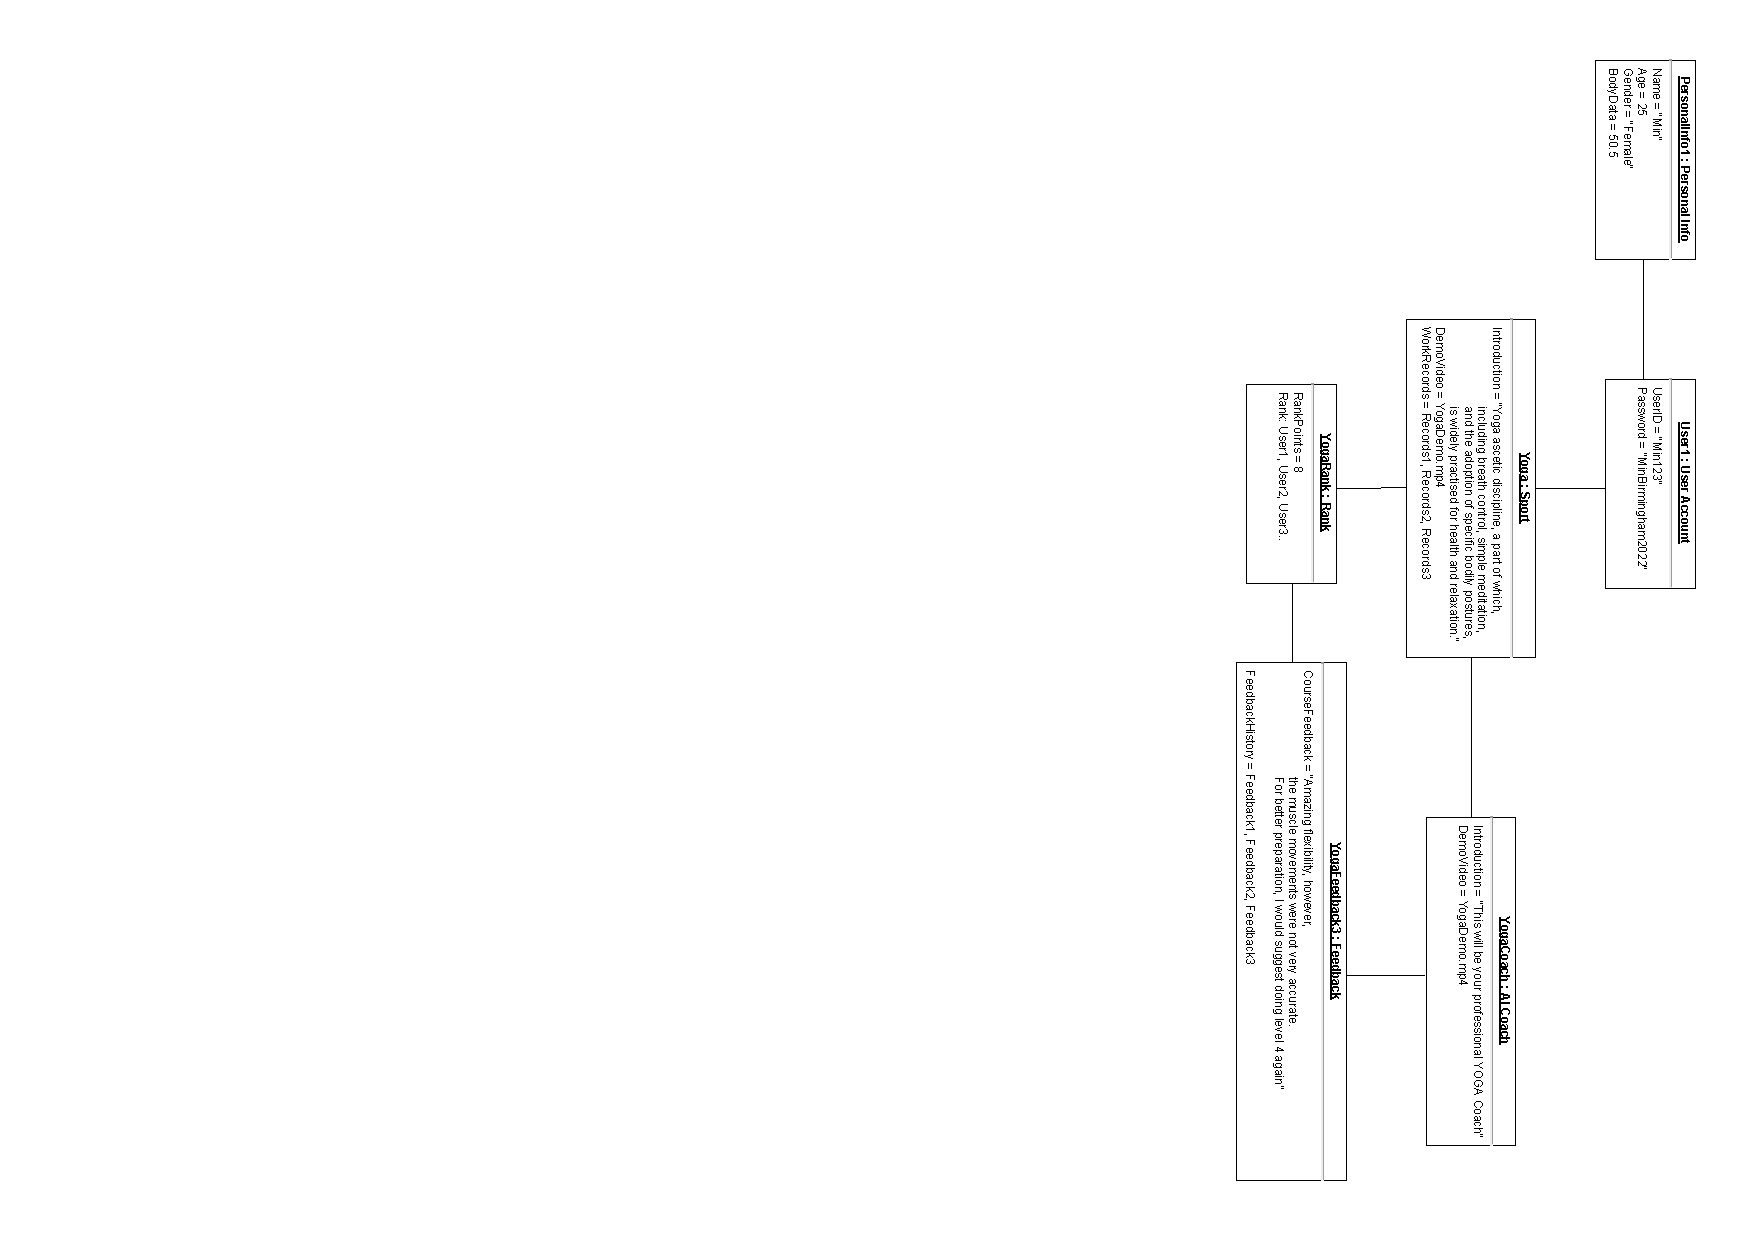
\includegraphics[width = 0.58\textwidth]{images/ObjectDiagram.pdf}
		\label{OD_Sport}
	\end{figure}

	\subsection{Sequence Diagram}

	\begin{figure}[H]
		\centering
		\caption*{\textbf{Diagram2.9} Sequence Diagram - Doing sports}
		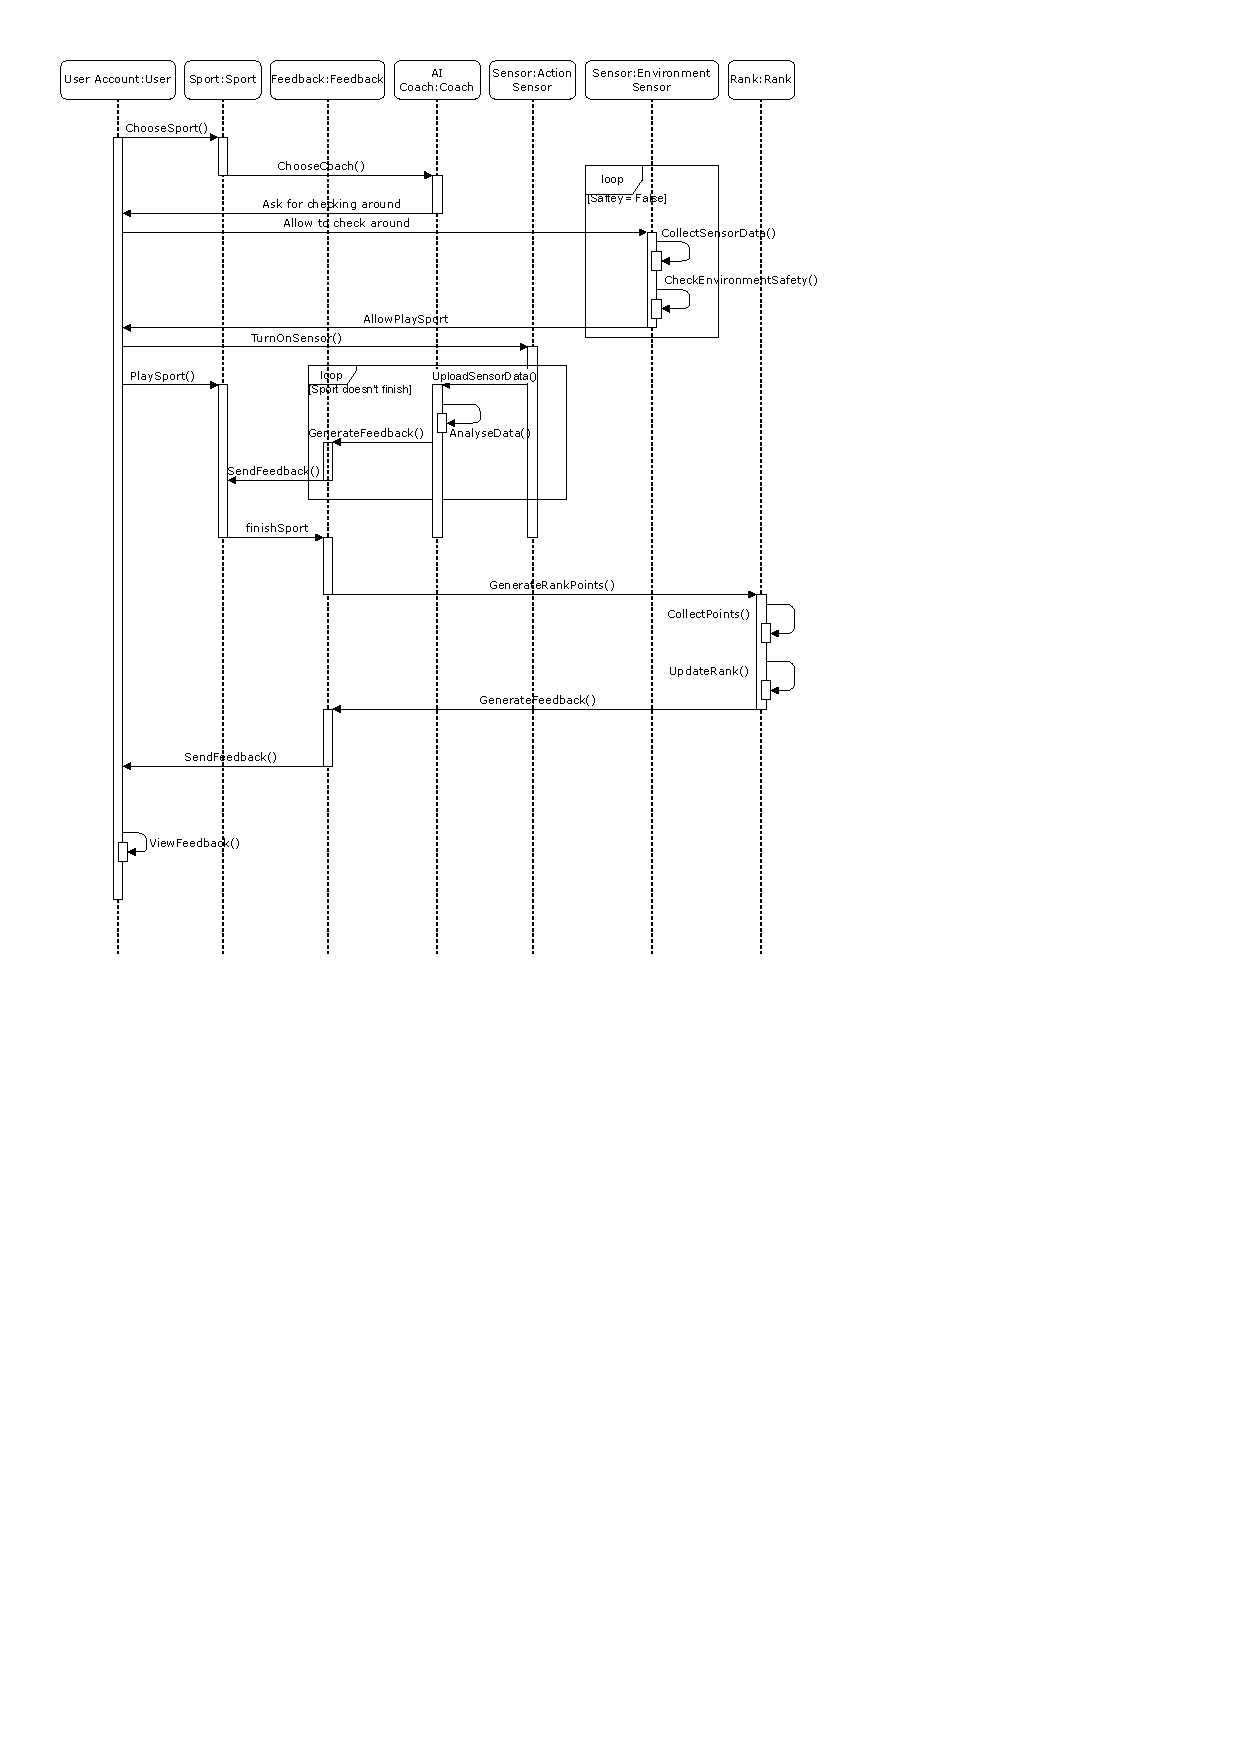
\includegraphics[width = 0.98\textwidth]{images/SequenceDiagram_Sport.pdf}
		\label{SD_Sport}
	\end{figure}

	\begin{figure}[H]
		\centering
		\caption*{\textbf{Diagram2.10} Sequence Diagram - Register}
		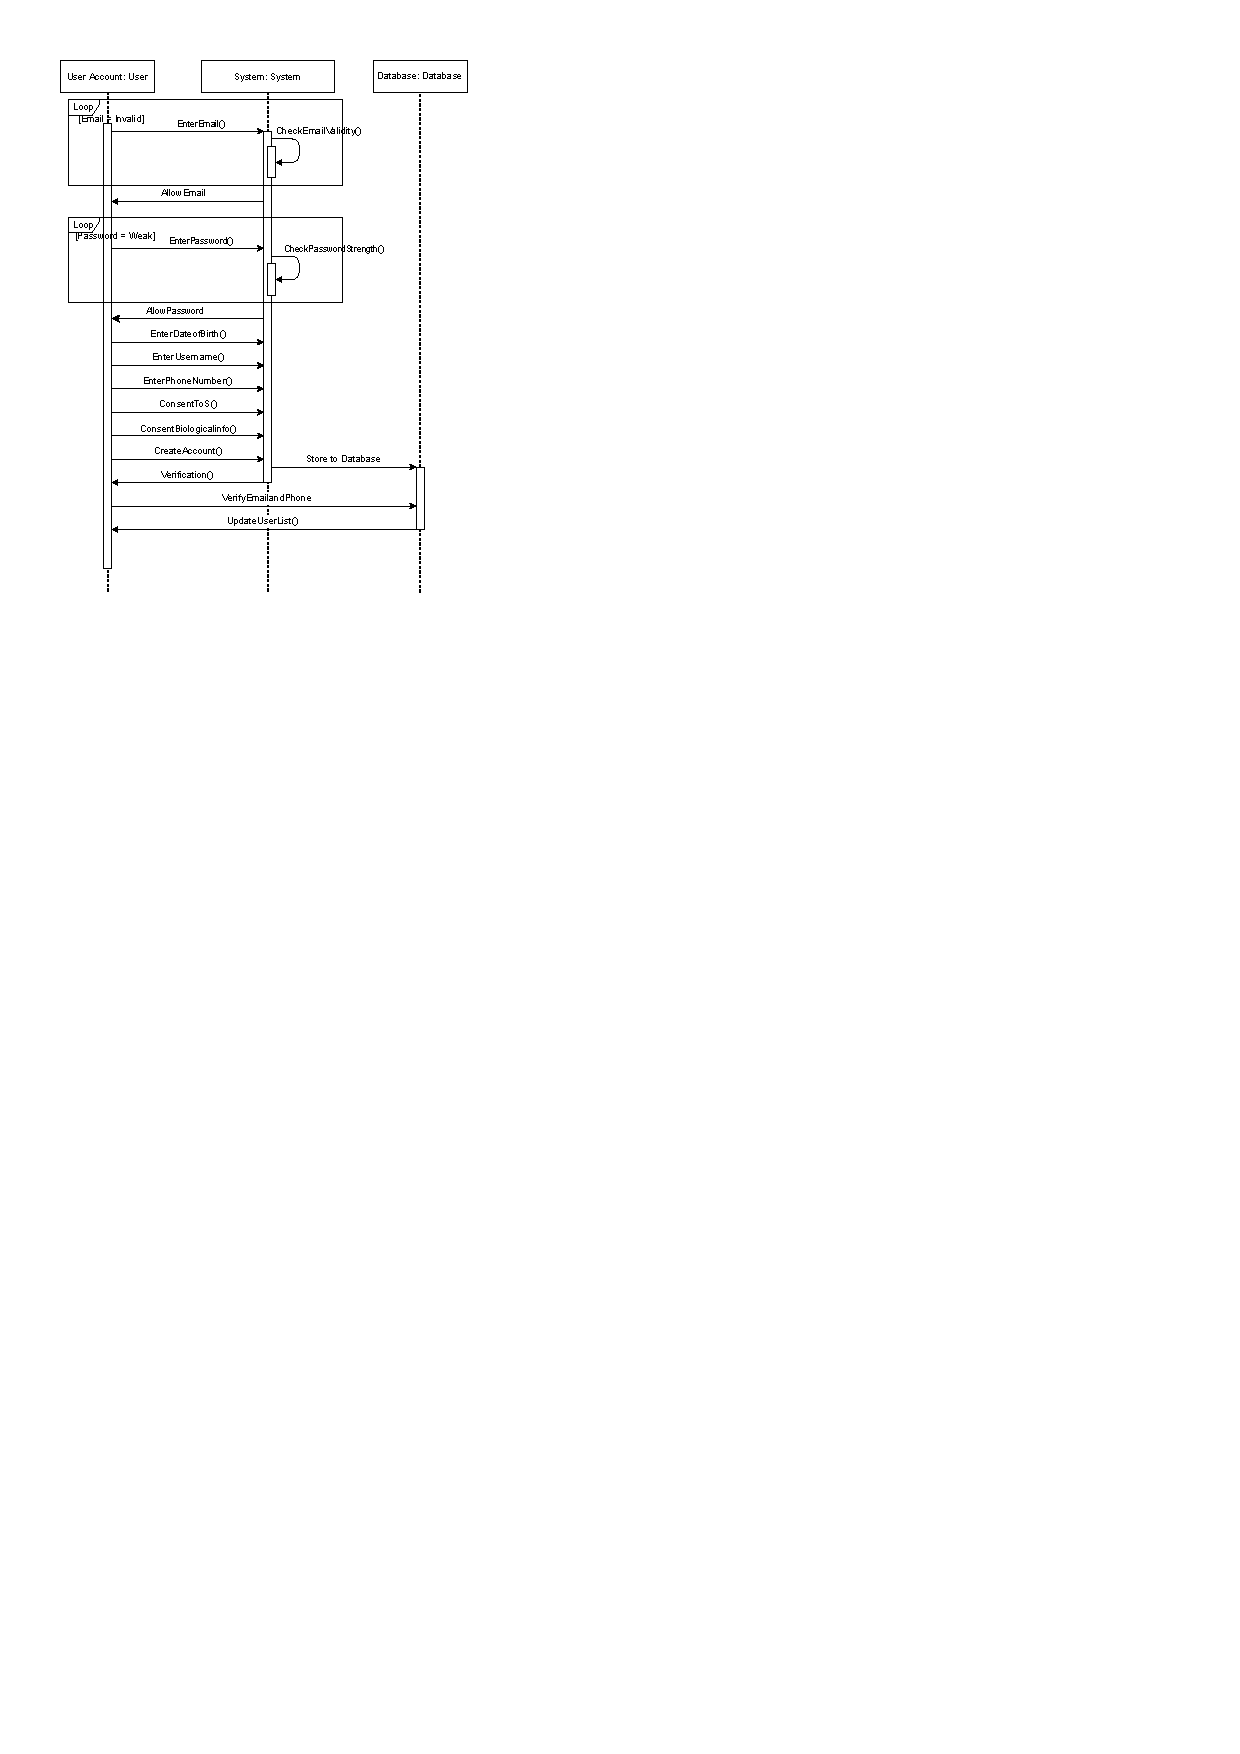
\includegraphics[width = 0.98\textwidth]{images/SequenceDiagram_Register.pdf}
		\label{SD_Register}
	\end{figure}

	\subsection{State Machine Diagram}

	\begin{figure}[H]
		\centering
		\caption*{\textbf{Diagram2.11} State Machine Diagram - Adding friends}
		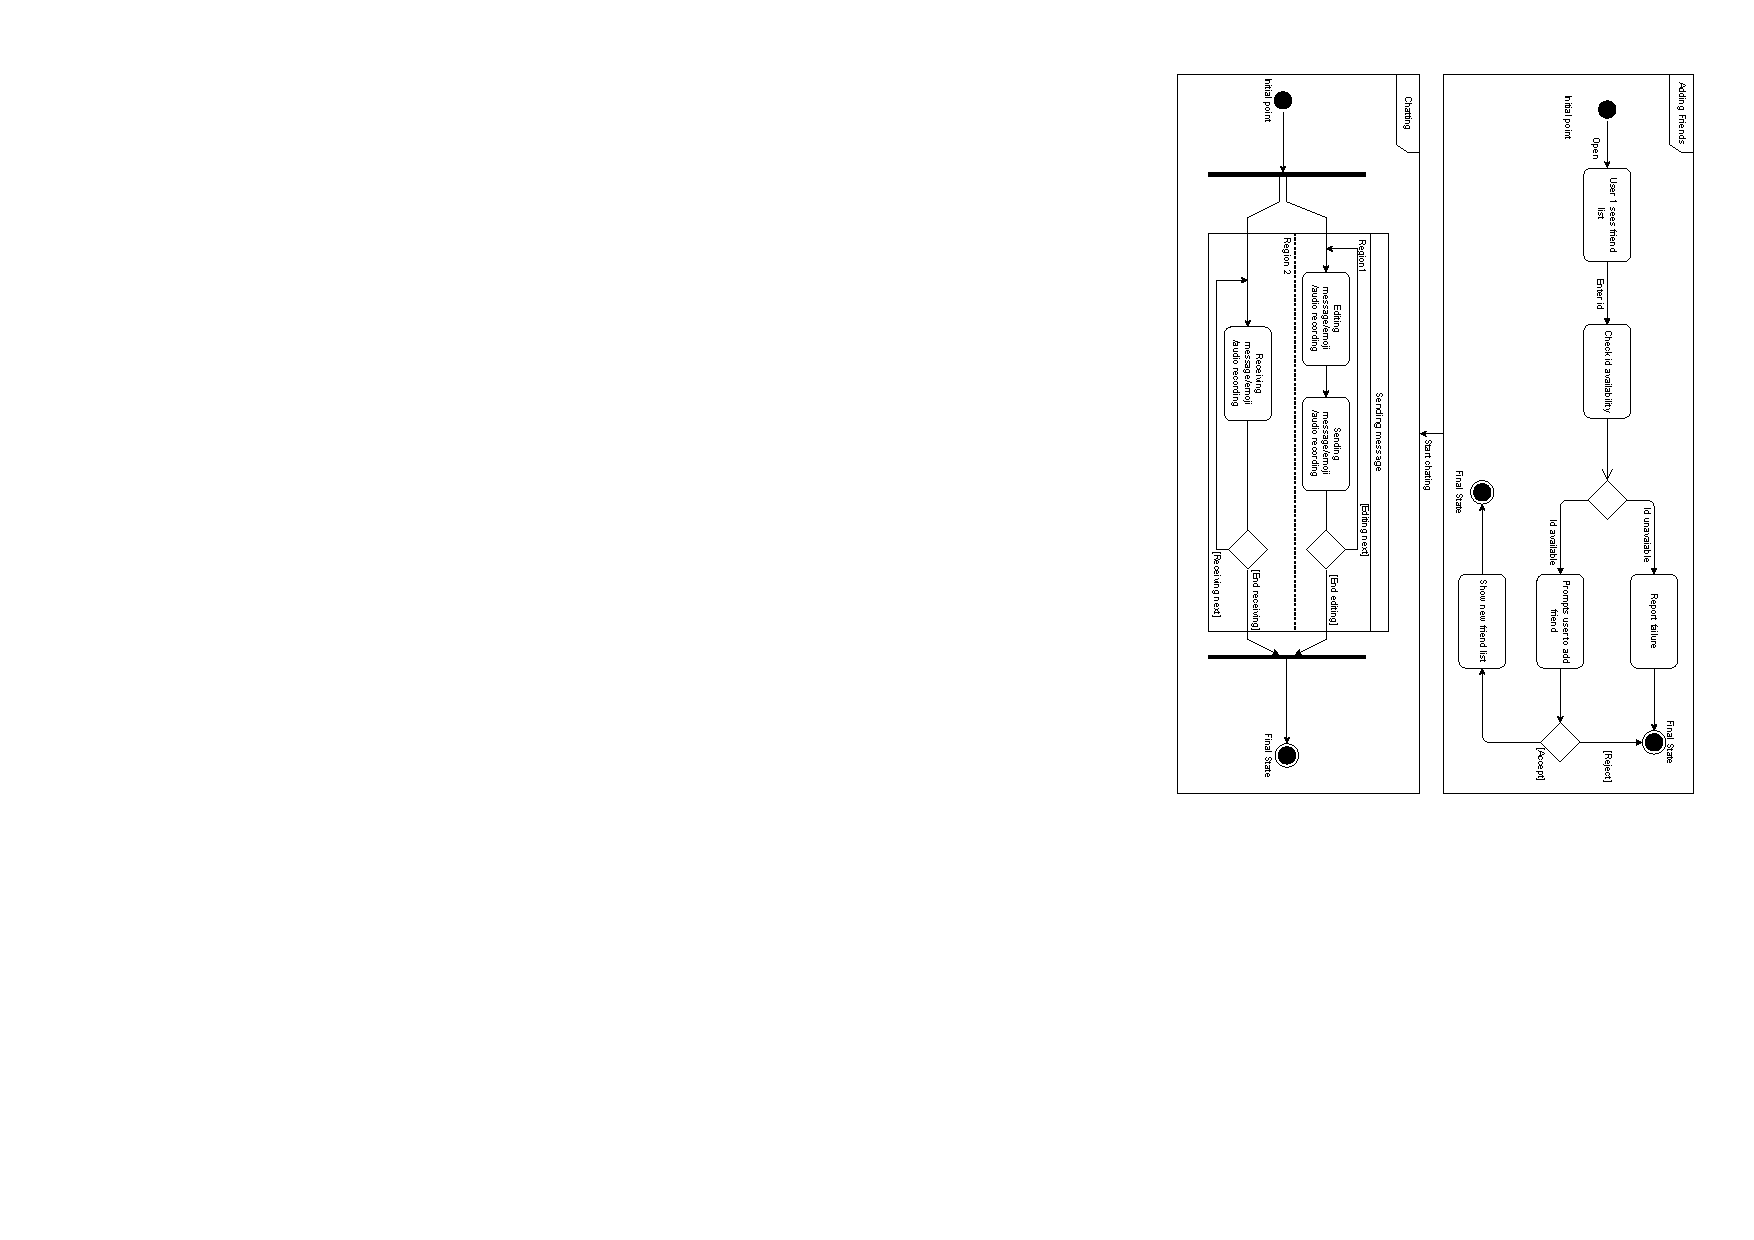
\includegraphics[width = 0.98\textwidth]{images/StateMachineDiagram_AddFriends_final.pdf}
		\label{SMD_AddFriend}
	\end{figure}

	\begin{figure}[H]
		\centering
		\caption*{\textbf{Diagram2.12} State Machine Diagram - Do sports}
		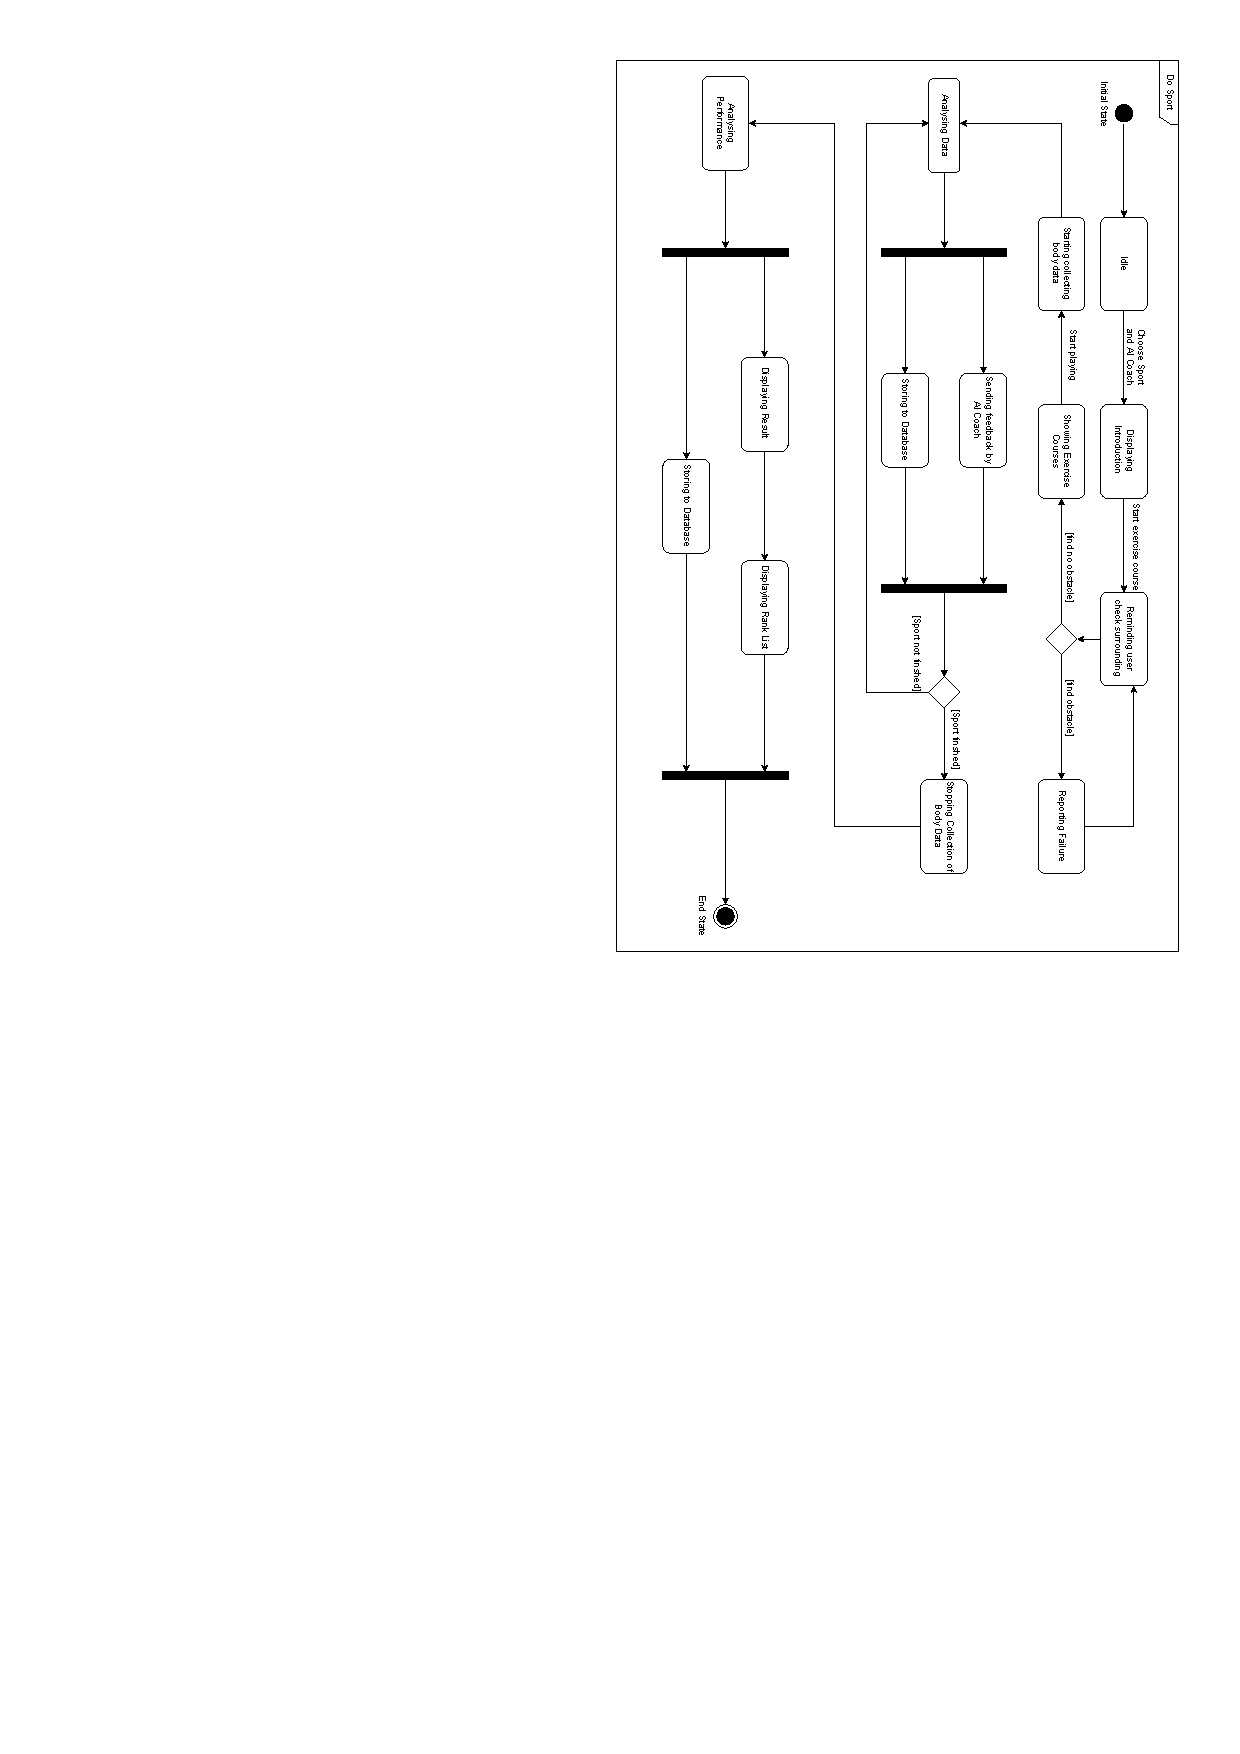
\includegraphics[width = 0.98\textwidth]{images/StateMachineDiagram_DoSport.pdf}
		\label{SMD_DoSport}
	\end{figure}

	\section{Software Architecture Style, Modelling and Evaluation}

	\subsection{UML Components Diagrams}

	\begin{figure}[H]
		\centering
		\caption*{\textbf{Diagram3.1} Components Diagram- Layered Style}
		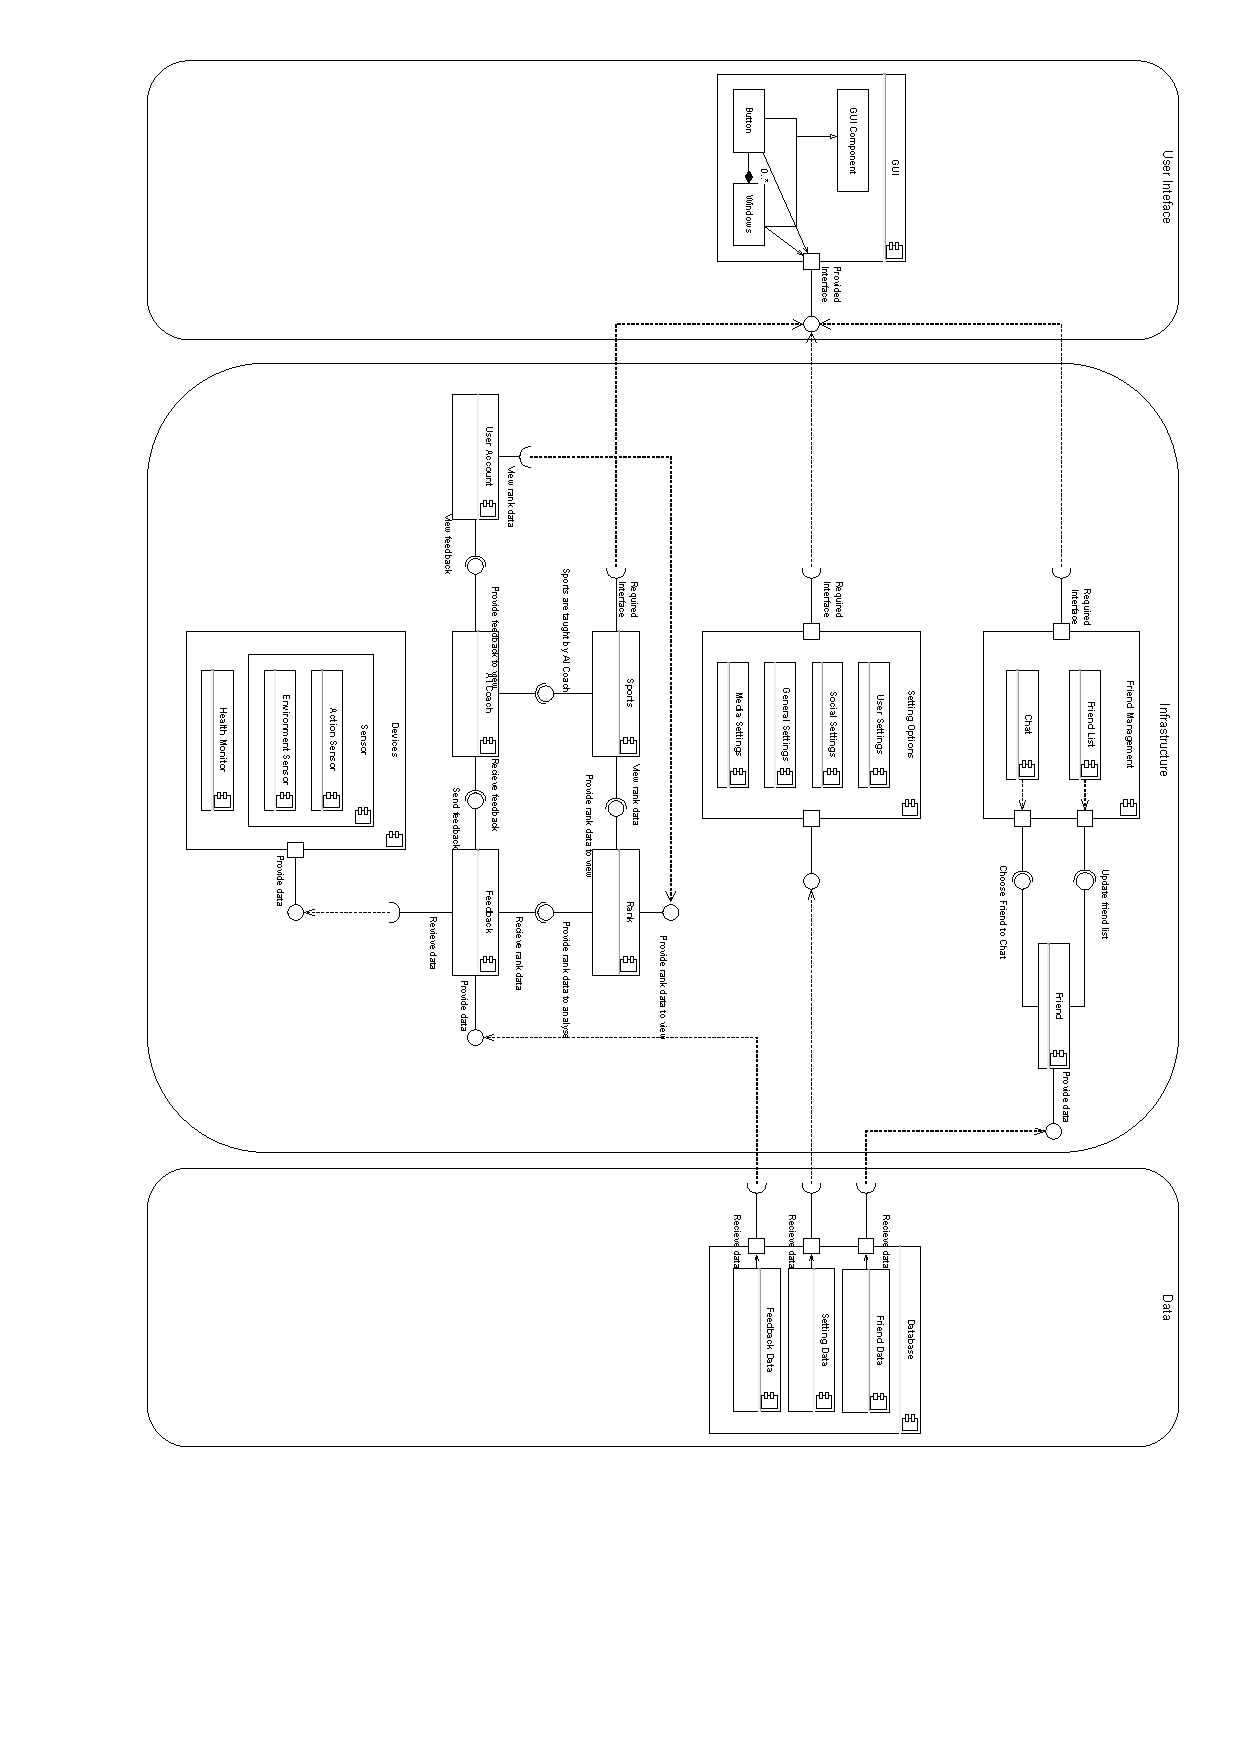
\includegraphics[width=0.95\textwidth]{images/ComponentsDiagram_Layered.pdf}
		\label{CD_L}
	\end{figure}

	\begin{figure}[H]
		\centering
		\caption*{\textbf{Diagram3.2} Components Diagram- Repository Architecture Style}
		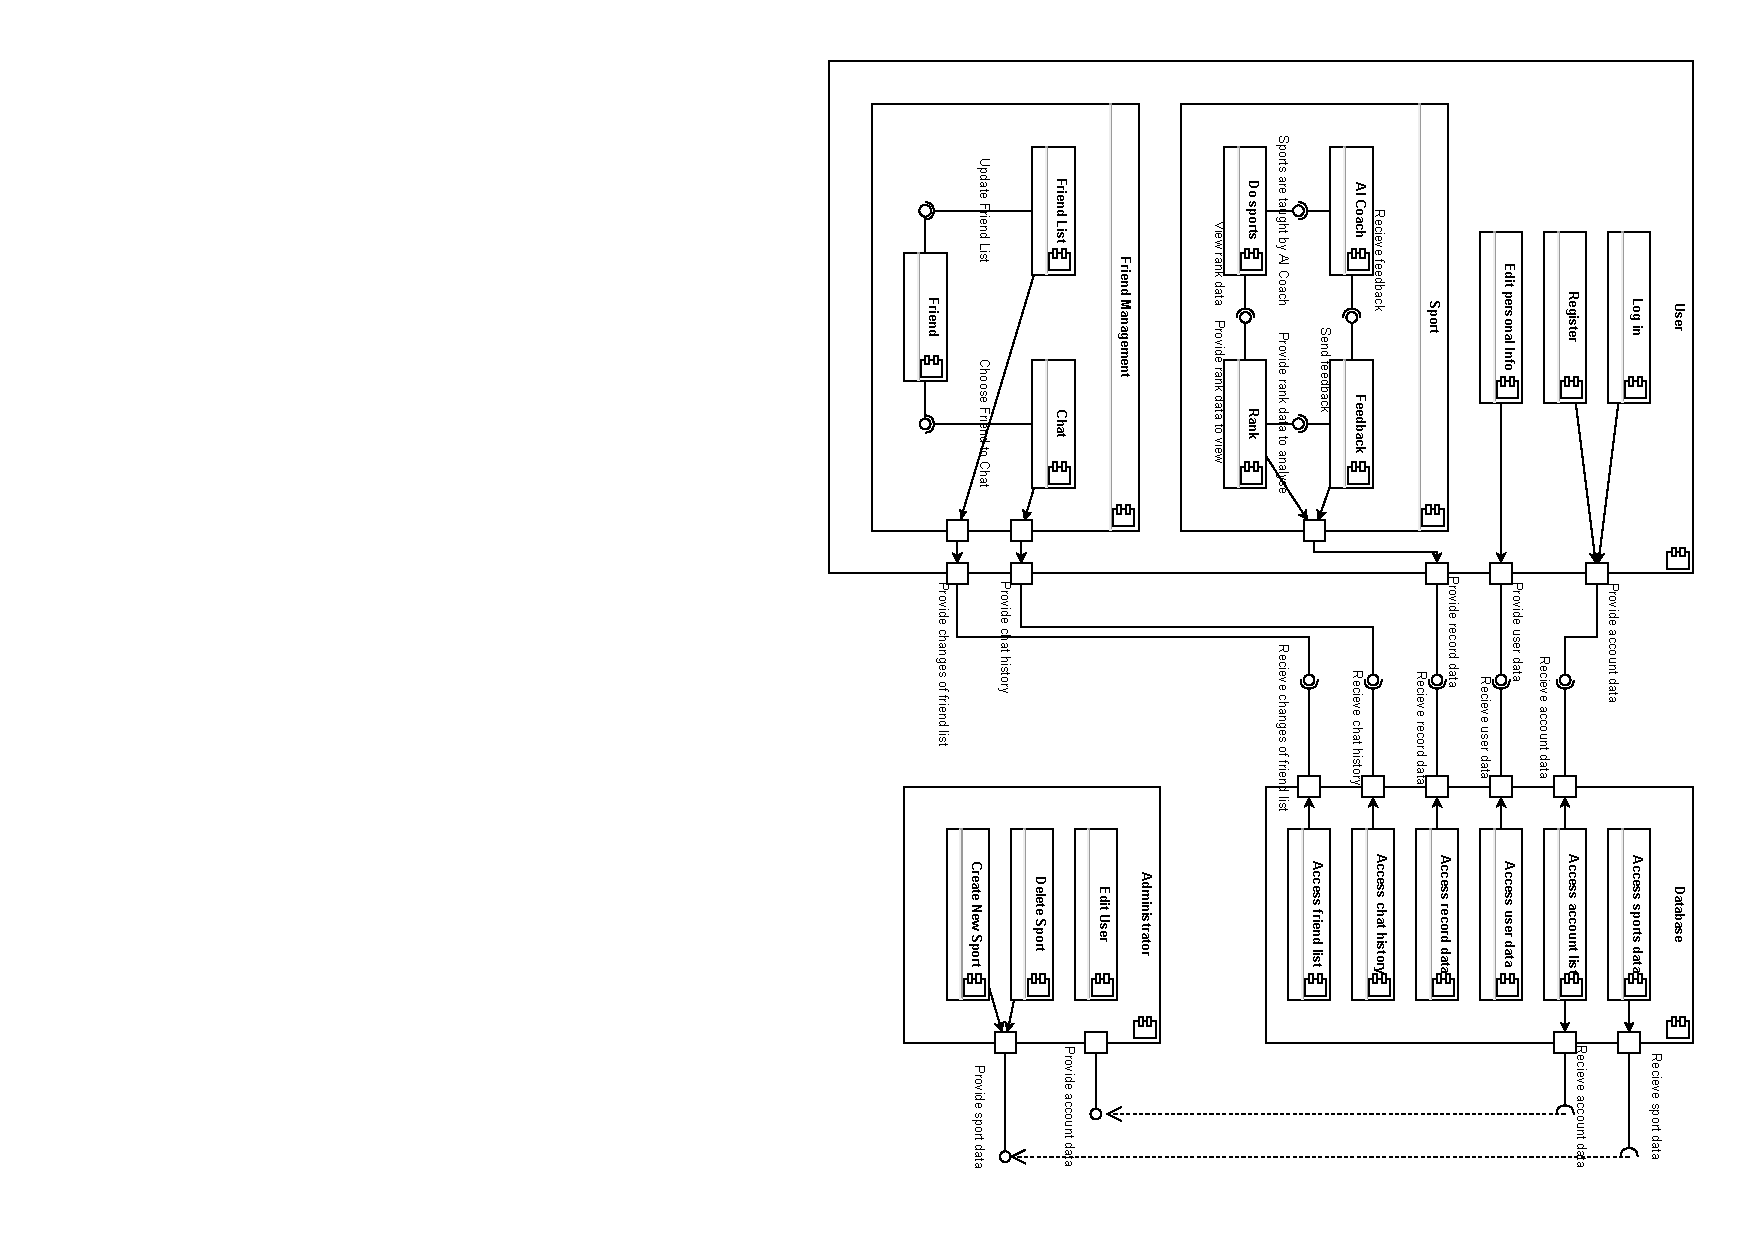
\includegraphics[width=1\textwidth]{images/ComponentsDiagram_Repository.pdf}
		\label{CD_RA}
	\end{figure}

	\subsection{Deployment Diagrams}

	\begin{figure}[H]
		\centering
		\caption*{\textbf{Diagram3.3} Deployment Diagram- Layered Style}
		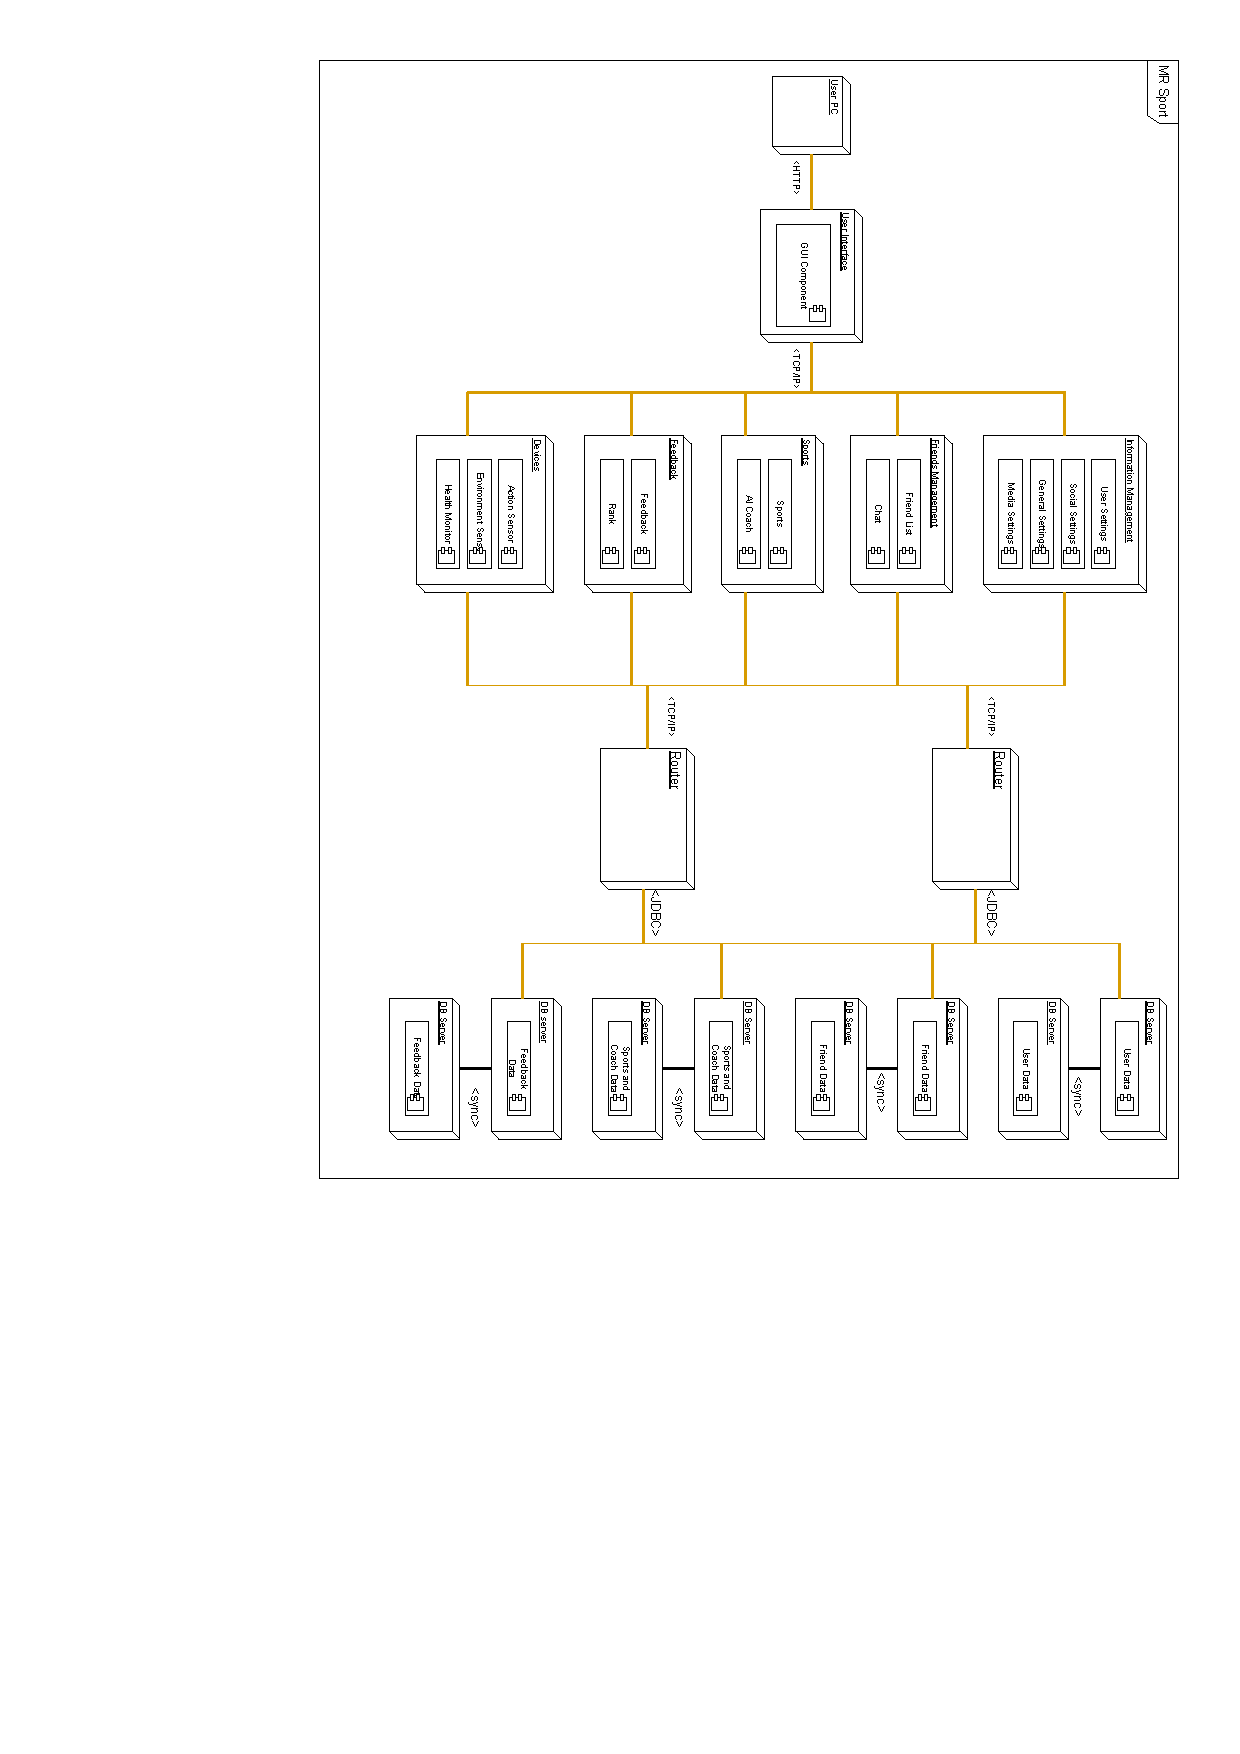
\includegraphics[width=1\textwidth]{images/DeploymentDiagram_Layered.pdf}
		\label{DD_L}
	\end{figure}

	\begin{figure}[H]
		\centering
		\caption*{\textbf{Diagram3.4} Deployment Diagram- Repository Architecture Style}
		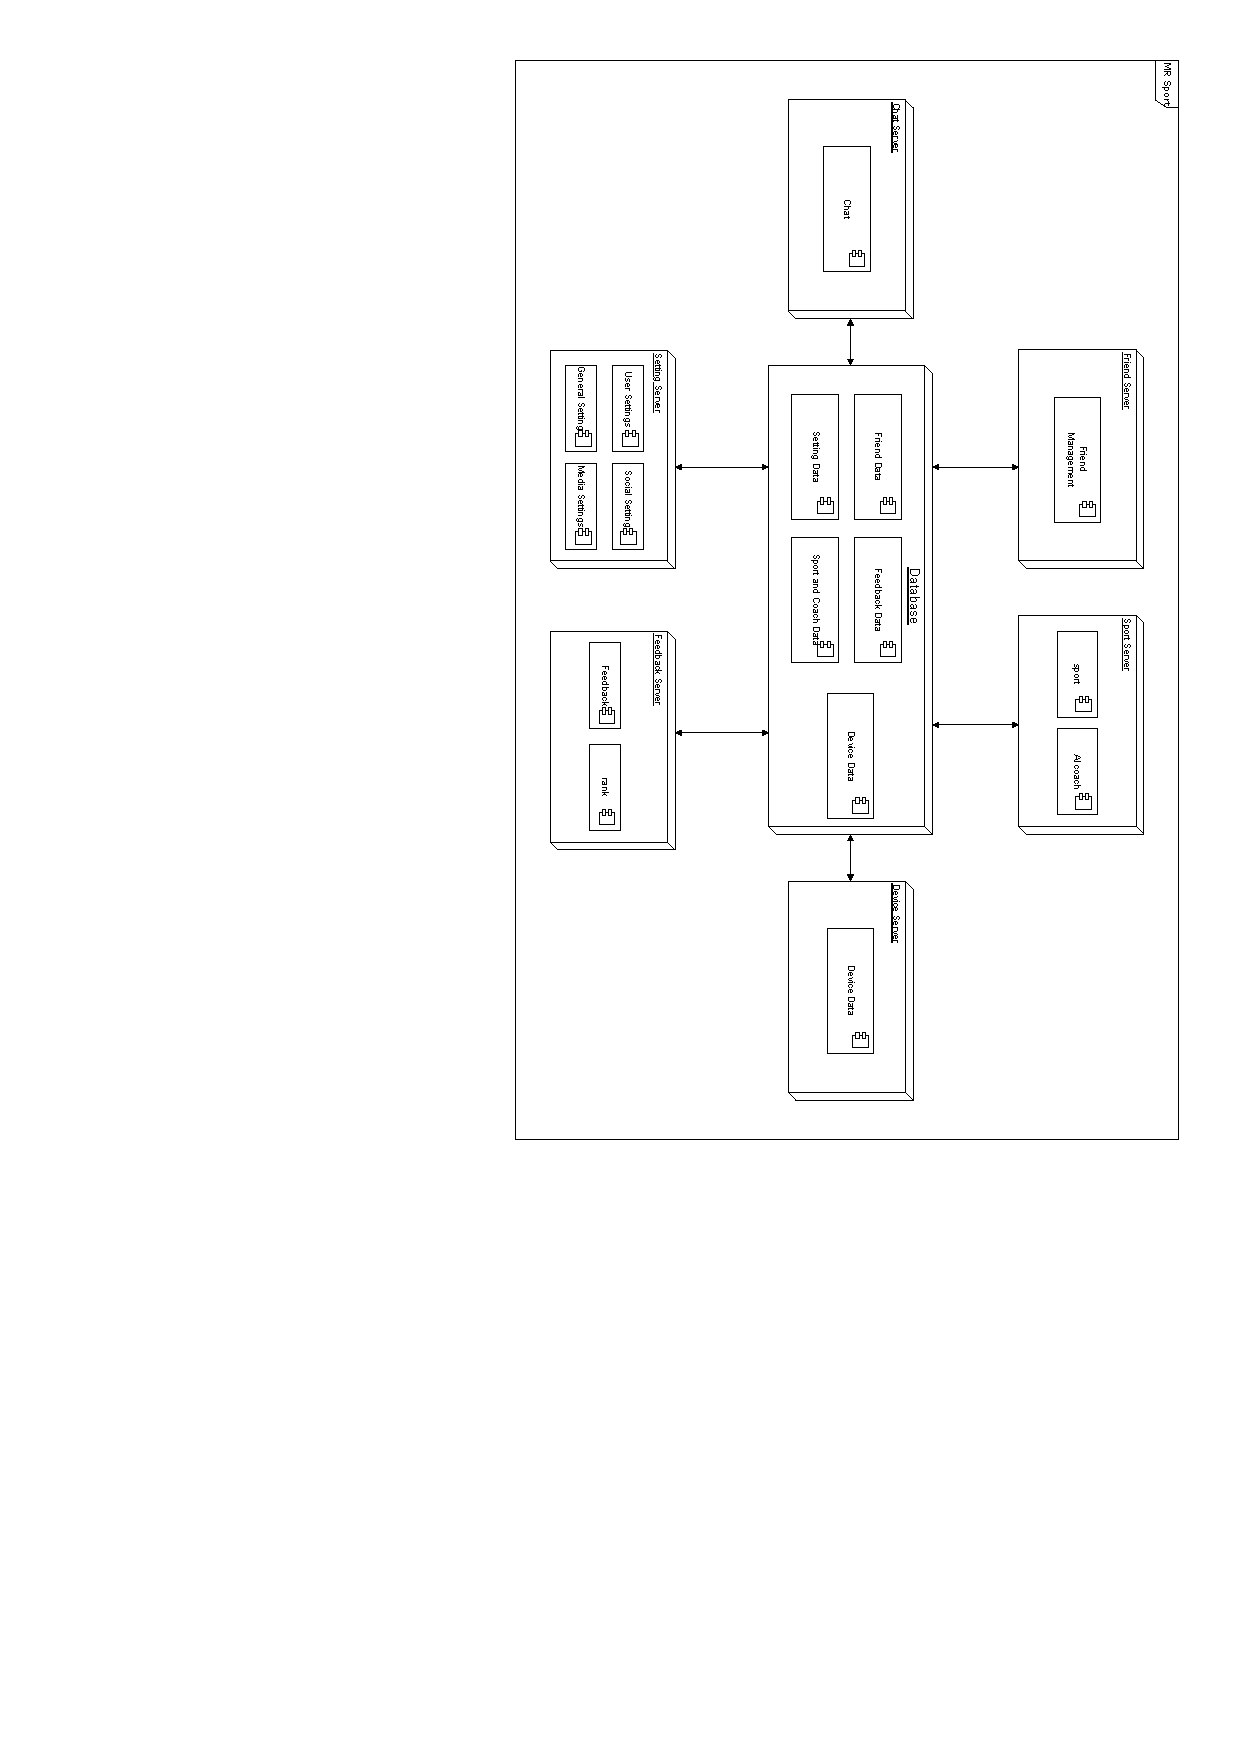
\includegraphics[width=1\textwidth]{images/DeploymentDiagram_Repository.pdf}
		\label{DD_RA}
	\end{figure}
	\newpage

	\subsection{Compare Architectures and Tradeoffs}

	Software architecture acts as the blueprint for the development of software, allowing the complexity of a system to be modelled, while establishing communication between components and connectors (Jaiswal, 2019; Qureshi et al., 2011)\cite{ref2,ref3}. The blueprint can be represented in various styles; this application has been demonstrated through both the `layered' and `repository' style of software architecture. Ideally, the system should perform well, be secure, be maintainable, allow iteration and scalability, be feasible and efficient; however actually implementing these qualities require trade-offs to be considered.\par
	A similarity both types of architecture exhibit is the capacity for scalability and iteration, due to both styles having the capability for loose coupling of components. However the repository (AKA blackboard) style is more accommodating for scalability as components and knowledge sources can be added and removed from the system without having to restructure the model; Whereas, this may be untrue for the layered style, as restructuring of layers and scaling of the entire application to accommodate changes at one specific layer is often required, thus scaling a layered model may be more resource intensive and less feasible (Akmel et al., 2017)\cite{ref1}. Due to the nature of the application, updates (more playable sports) and new features will be implemented so scalability, and in turn economic feasibility, is a priority.\par
	The layered architecture style provides a higher level of security due to the concept of onion skinning, by compounding layers of protection on each layer of the system, creating almost an onion skin affect. On the other hand, the flexibility that the repository architecture provides for allowing the addition of new components to the main repository may reduce the overall confidence in this model's system security. However, due to how independent components in a repository system are, the system may be able to continue to function even if one component breaks or the function becomes degraded; this could be useful in a multi-functioning app such as the one proposed, for example if the co-operative feature of the app is currently under maintenance, the user can still access other services such as AI coaching and exchanging messages with friends.\par
	Overall, for this project there is preference towards the repository architecture style due to feasibility and flexibility the style allows for the application, however there is also a use-case for the layered architecture style as it also accommodates for features the repository style does not do as well.

	\newpage
	\section{Software Testing}

	\subsection{Introduction}

	The system will allow users to train and play sports of their choice with the help of an AI virtual coach through creating an account with the Metaverse Sport application and devices for scanning their body and surrounding as well as the system measuring data in relation to the sports performance which will be reflected in the user's ranks. This will allow the users to track their performance and receive feedback from their AI virtual coach. In addition, the system will allow the users to add friends and chat with each other as well as participate in competitions with people around the world.\par
	The system will be testified to ensure that it conforms to functional and non-functional requirements as well as it meets its quality specifications defined by the client. Any critical bugs or issues should be identified and fixed before going live. These include:
	\begin{itemize}[itemindent=2em]
		\item[$\bullet$] Response time required when the user logs in to the system
		\item[$\bullet$] Response time to analyse and scan for the obstacles in the surroundings and send a reminder to the user to confirm the safety of their surroundings
		\item[$\bullet$] The system will make a backup within the expected time frame i.e., 5 minutes to prevent data loss 
	\end{itemize}

	\subsection{Test Items}

	The systems to be tested include the frontend software interface along with the backend AI Data analyse. These sytem should be tested in the latest version of MR devices

	\subsection{Features to be tested}

	Features to be tested include the following:
	\begin{enumerate}[itemindent=2em]
		\item As a user, logging into the system
		\item As the system, checking the surroundings
		\item As a user, doing sport
		\item As a user, checking the rank
		\item As a user, adding friends
		\item As a user, Chatting
		\item As the system, generating feedback correctly
		\item As the system, validating the user's information within 5 seconds when the user login
		\item As the system, allowing users to backup account data locally or online
		\item As a user, share ranking scores to other social media
	\end{enumerate}

	\subsection{Features not to be tested}

	Data collection efficiency and accuracy of sensor will not be tested. We do need an extra testing tool for testing this functionality. Data analyse and comparation take a lot of time.

	\subsection{Approach}

	Test planning will be carried out in four stages.
	\begin{itemize}[itemindent=2em]
		\item[$\bullet$] Unit testing: The programmers use the white-box testing and test coverage techniques to test the unit and get the unit test report.
		\item[$\bullet$] Integration testing: The programmers and testers use the White and Black Box testing to test the integration, and get the integration test report
		\item[$\bullet$] System testing: The testers will test system and get the system test report
		\item[$\bullet$] Acceptance testing: The users use black-box testing to test acceptance and get the user acceptance test report
	\end{itemize}\par
	The quality team will allocated all the reports. After analyzing and marking the test results, the quality team will feed back the results to the developers. The developers make modifications to fix it and the corresponding testing departments retest it. Until the test passes

	\subsection{Item Pass/Fail Criteria}
	{\footnotesize\noindent\begin{tabular}{|p{0.1\linewidth}|p{0.2\linewidth}|p{0.2\linewidth}|p{0.2\linewidth}|p{0.2\linewidth}|} 
	   	\hline
		\textbf{Test Case ID} & \textbf{Test description} & \textbf{Test steps} & \textbf{Test Data} & \textbf{Expected result} \\
		\hline
		TD-1\_1 & \multicolumn{1}{|l|}{\makecell[l]{Verify the login with valid \\userID and password}}																						& \multicolumn{1}{|l|}{\makecell[l]{Go to Metaverse Virtual \\Sport application;\\Enter UserID;\\Enter PasswordClick;\\ Submit}}																																														& \multicolumn{1}{|l|}{\makecell[l]{UserID: Min\\Password: ABC123£\$}}				& \multicolumn{1}{|l|}{\makecell[l]{The user should be able\\ to log in within 5 seconds.}}\\
		\hline
		TD-2\_1 & \multicolumn{1}{|l|}{\makecell[l]{The system analyses and\\ checks the safety of the\\ surrounding as well as\\sends a reminder to the\\user to check the\\surrounding}}	& \multicolumn{1}{|l|}{\makecell[l]{Environment sensor scans \\the surroundings and waits\\ for the user to confirm it\\ is safe}}																																														& \multicolumn{1}{|l|}{\makecell[l]{Sensor data;\\ user confirmation data}} 		& \multicolumn{1}{|l|}{\makecell[l]{The environment sensor \\should be able to scan any\\ obstacles and send a \\reminder to the use}}\\
		\hline
		TD-3\_1 & \multicolumn{1}{|l|}{\makecell[l]{play the chosen sport}}																													& \multicolumn{1}{|l|}{\makecell[l]{login;\\ select a specific sport and coach}}																																																													& \multicolumn{1}{|l|}{\makecell[l]{chosen sport data}} 							& \multicolumn{1}{|l|}{\makecell[l]{User can play the sport \\that they chose}}\\
		\hline
		TD-3\_2 & \multicolumn{1}{|l|}{\makecell[l]{AI Coach analysis}}																														& \multicolumn{1}{|l|}{\makecell[l]{Select sport;\\ select coach;\\ play sport}}																																																										& \multicolumn{1}{|l|}{\makecell[l]{User health data;\\ User movements' data}} 		& \multicolumn{1}{|l|}{\makecell[l]{AI Coach should respond \\with suitable info based\\ on the users' movement\\ and health data}}\\
		\hline
		TD-4\_1 & \multicolumn{1}{|l|}{\makecell[l]{Getting the rank \\assigned to the user}}																								& \multicolumn{1}{|l|}{\makecell[l]{play sport;\\ get points based on actions;\\ finish sport}}																																																						& \multicolumn{1}{|l|}{\makecell[l]{Users' movements data}} 						& \multicolumn{1}{|l|}{\makecell[l]{rank is assigned to the \\user based on how many \\points were collected}}\\
		\hline
		TD-5\_1 & \multicolumn{1}{|l|}{\makecell[l]{Add other users to \\friend list}}																										& \multicolumn{1}{|l|}{\makecell[l]{User1 go to the friend list page;\\Click `search' button;\\Enters user ID of User2 in the\\ search bar;\\Click `send friend request' \\button;\\User2 receive the request of \\adding friend;\\User2 clicks `accept' button}}						& \multicolumn{1}{|l|}{\makecell[l]{Friend list of User1;\\Friend list of User2}} 	& \multicolumn{1}{|l|}{\makecell[l]{User2 is in the friend list\\ of User1;\\User1 is in the friend list\\ of User2}}\\
		\hline
	\end{tabular}}
	\newpage
	{\footnotesize\noindent\begin{tabular}{|p{0.1\linewidth}|p{0.2\linewidth}|p{0.2\linewidth}|p{0.2\linewidth}|p{0.2\linewidth}|} 
	   	\hline
		TD-6\_1 & \multicolumn{1}{|l|}{\makecell[l]{Chat with other users \\in friend list}}																								& \multicolumn{1}{|l|}{\makecell[l]{User1 go to the friend list page;\\Click `User2' tab;\\View the information page of\\ User2;\\Click `chat' button;\\Edit message and click `send' \\button;\\User2 receive message from \\User1;\\Edit message and click `send' \\button;\\User1 receive message from \\User2 }}	& \multicolumn{1}{|l|}{\makecell[l]{Chatting Data}} 								& \multicolumn{1}{|l|}{\makecell[l]{All messages are delivered\\ correctly between User1 \\and User2}}\\
		\hline
		TD-7\_1 & \multicolumn{1}{|l|}{\makecell[l]{Generating feedback \\correctly-Generate\\performance info}}																			& \multicolumn{1}{|l|}{\makecell[l]{Finish playing sports;\\Click finish button;\\Choose review performance\\ info }}																																																	& \multicolumn{1}{|l|}{\makecell[l]{User performance data}} 						& \multicolumn{1}{|l|}{\makecell[l]{Properly generate feedback\\ based on user performance}}\\
		\hline
		TD-7\_2 & \multicolumn{1}{|l|}{\makecell[l]{Generating feedback \\correctly}}																										& \multicolumn{1}{|l|}{\makecell[l]{Finish playing sports;\\Click finish button;\\Choose generate feedback}}																																																			& \multicolumn{1}{|l|}{\makecell[l]{User performance data}} 						& \multicolumn{1}{|l|}{\makecell[l]{Properly generate feedback\\ based on user performance}}\\
		\hline
		TD-8\_1 & \multicolumn{1}{|l|}{\makecell[l]{Validate the user's \\information}}																										& \multicolumn{1}{|l|}{\makecell[l]{Fill in user information;\\Click submit button;\\Validate in the database}}																																																			& \multicolumn{1}{|l|}{\makecell[l]{User account data}} 							& \multicolumn{1}{|l|}{\makecell[l]{User account data is\\ validated correctly}}\\
		\hline
		TD-8\_2 & \multicolumn{1}{|l|}{\makecell[l]{Validate the user's \\information-Meet \\the time limit}}																				& \multicolumn{1}{|l|}{\makecell[l]{Fill in user information;\\Click submit button;\\Validate in the database;\\Return validation time}}																																												& \multicolumn{1}{|l|}{\makecell[l]{User account data}} 							& \multicolumn{1}{|l|}{\makecell[l]{Validating the user's\\ information within 5 \\seconds when the user \\login}}\\
		\hline
		TD-9\_1 & \multicolumn{1}{|l|}{\makecell[l]{Backup the account data\\ locally}}																										& \multicolumn{1}{|l|}{\makecell[l]{Go setting page;\\open account setting;\\click `backup locally' button}}																																																			& \multicolumn{1}{|l|}{\makecell[l]{User account data}} 							& \multicolumn{1}{|l|}{\makecell[l]{User account data is stored\\ in device correctly and \\safely}}\\
		\hline
		TD-9\_2 & \multicolumn{1}{|l|}{\makecell[l]{Backup the account data\\ online}}																										& \multicolumn{1}{|l|}{\makecell[l]{Go setting page;\\open account setting;\\click `backup online' button}}																																																				& \multicolumn{1}{|l|}{\makecell[l]{User account data}} 							& \multicolumn{1}{|l|}{\makecell[l]{User account data is stored\\ online correctly and safely}}\\
		\hline
		TD-10\_1 & \multicolumn{1}{|l|}{\makecell[l]{Share ranking scores to \\social media: \\Generate shared info}}																		& \multicolumn{1}{|l|}{\makecell[l]{Choose the ranking score\\ of one sport;\\Click share button}}																																																						& \multicolumn{1}{|l|}{\makecell[l]{Ranking score: 99}} 							& \multicolumn{1}{|l|}{\makecell[l]{Ranking score is fetched\\ correctly and generate\\ suitable shared info}}\\
		\hline
		TD-10\_2 & \multicolumn{1}{|l|}{\makecell[l]{Share ranking scores to \\social media: \\Share to friend}}																			& \multicolumn{1}{|l|}{\makecell[l]{Choose the ranking score\\ of one sport;\\Click share button;\\Choose friend}}																																																		& \multicolumn{1}{|l|}{\makecell[l]{Ranking score: 99}} 							& \multicolumn{1}{|l|}{\makecell[l]{Shared info is sent to \\correct person}}\\
		\hline
	\end{tabular}}

	\subsection{Exit Criteria}
	
	95\% of the test cases should pass and there are no failed critical cases.

	\subsection{Assumptions}

	We already have mature software development and testing technology.

	\newpage

	\section{Usability and Prototyping}

	\subsection{Interactive Prototype}

	\begin{figure}[H]
		\centering
		\caption*{\textbf{Diagram5.1} UI- Login}
		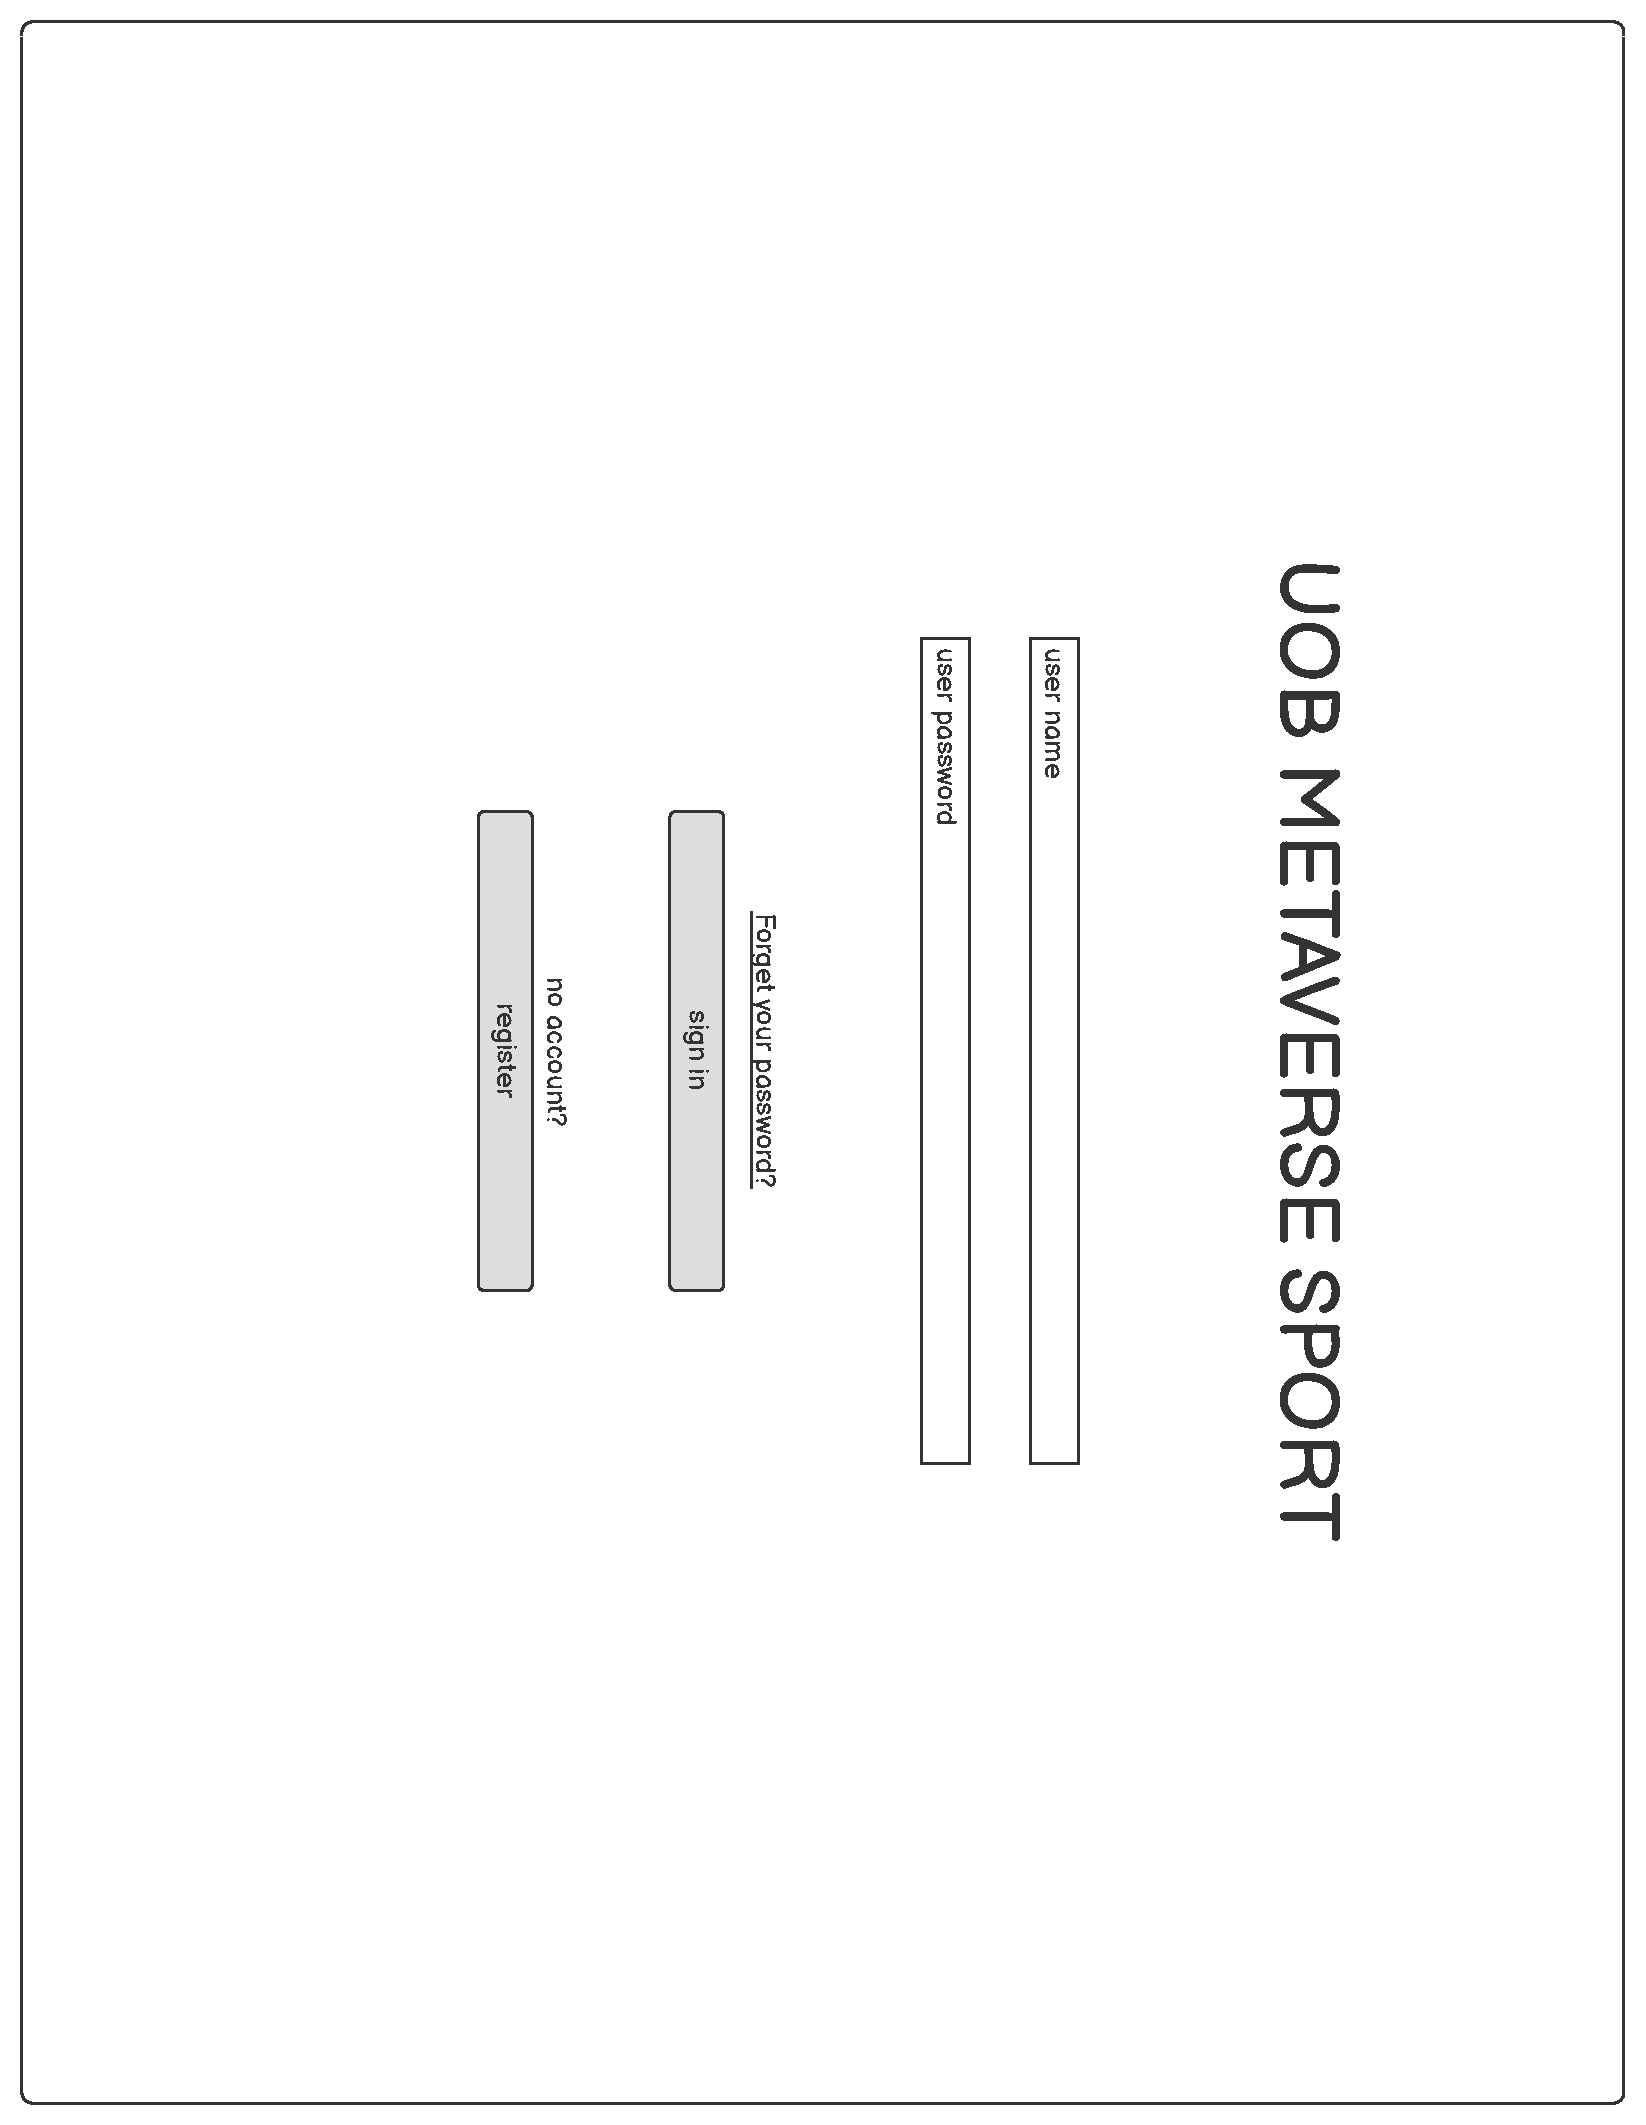
\includegraphics[width=1\textwidth]{images/UI_Final/UI_Final_1.pdf}
		\label{UI_1}
	\end{figure}

	\begin{figure}[H]
		\centering
		\caption*{\textbf{Diagram5.2} UI- Choose Sport}
		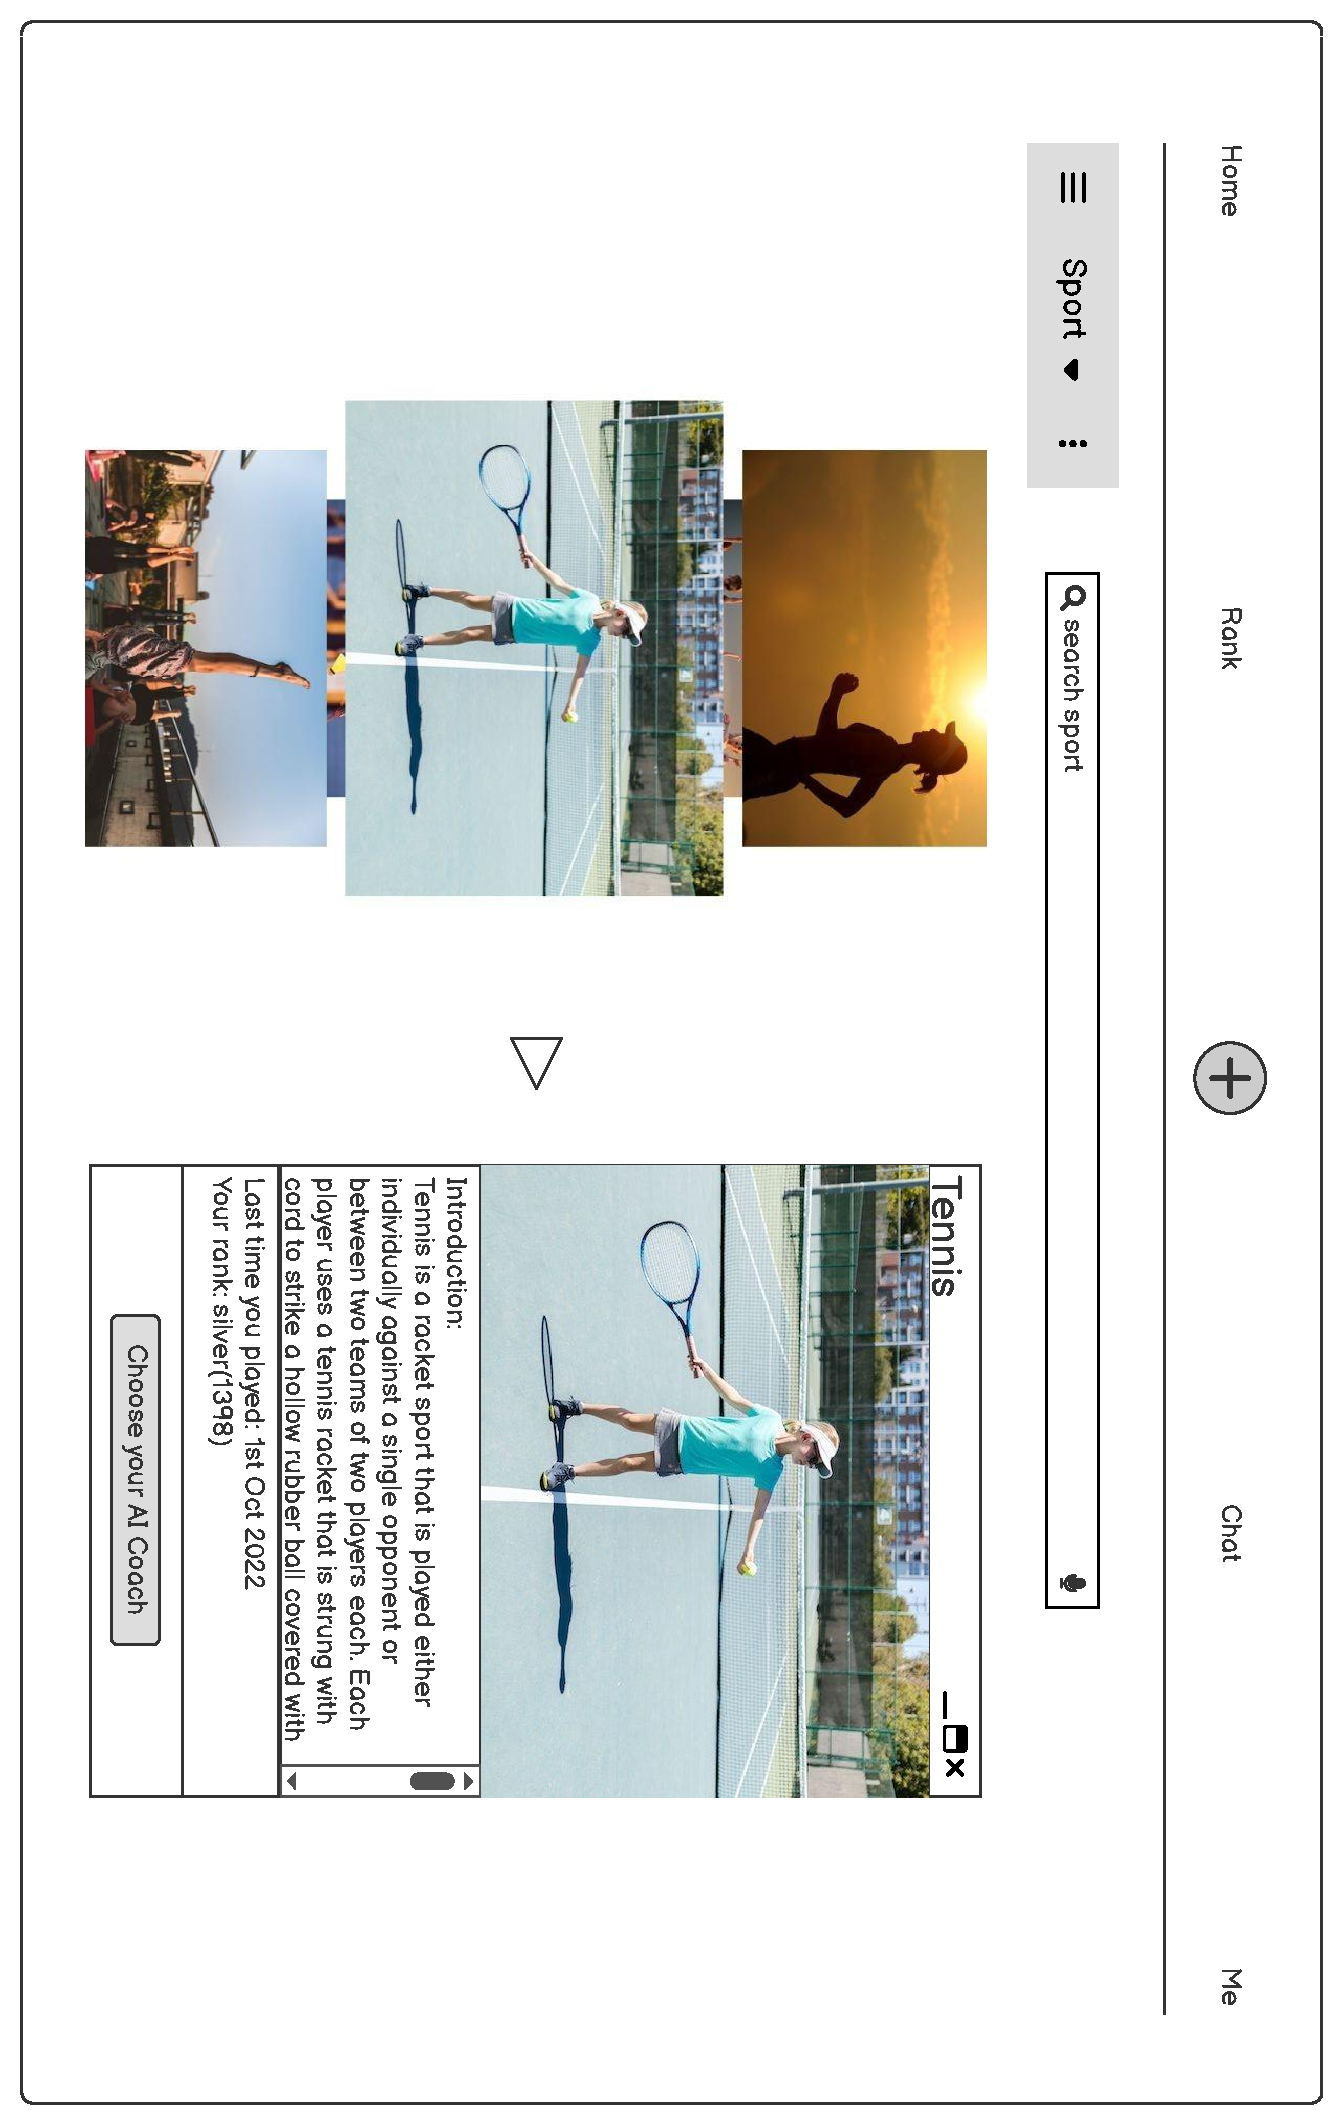
\includegraphics[width=1\textwidth]{images/UI_Final/UI_Final_2.pdf}
		\label{UI_2}
	\end{figure}

	\begin{figure}[H]
		\centering
		\caption*{\textbf{Diagram5.3} UI- Choose Coach}
		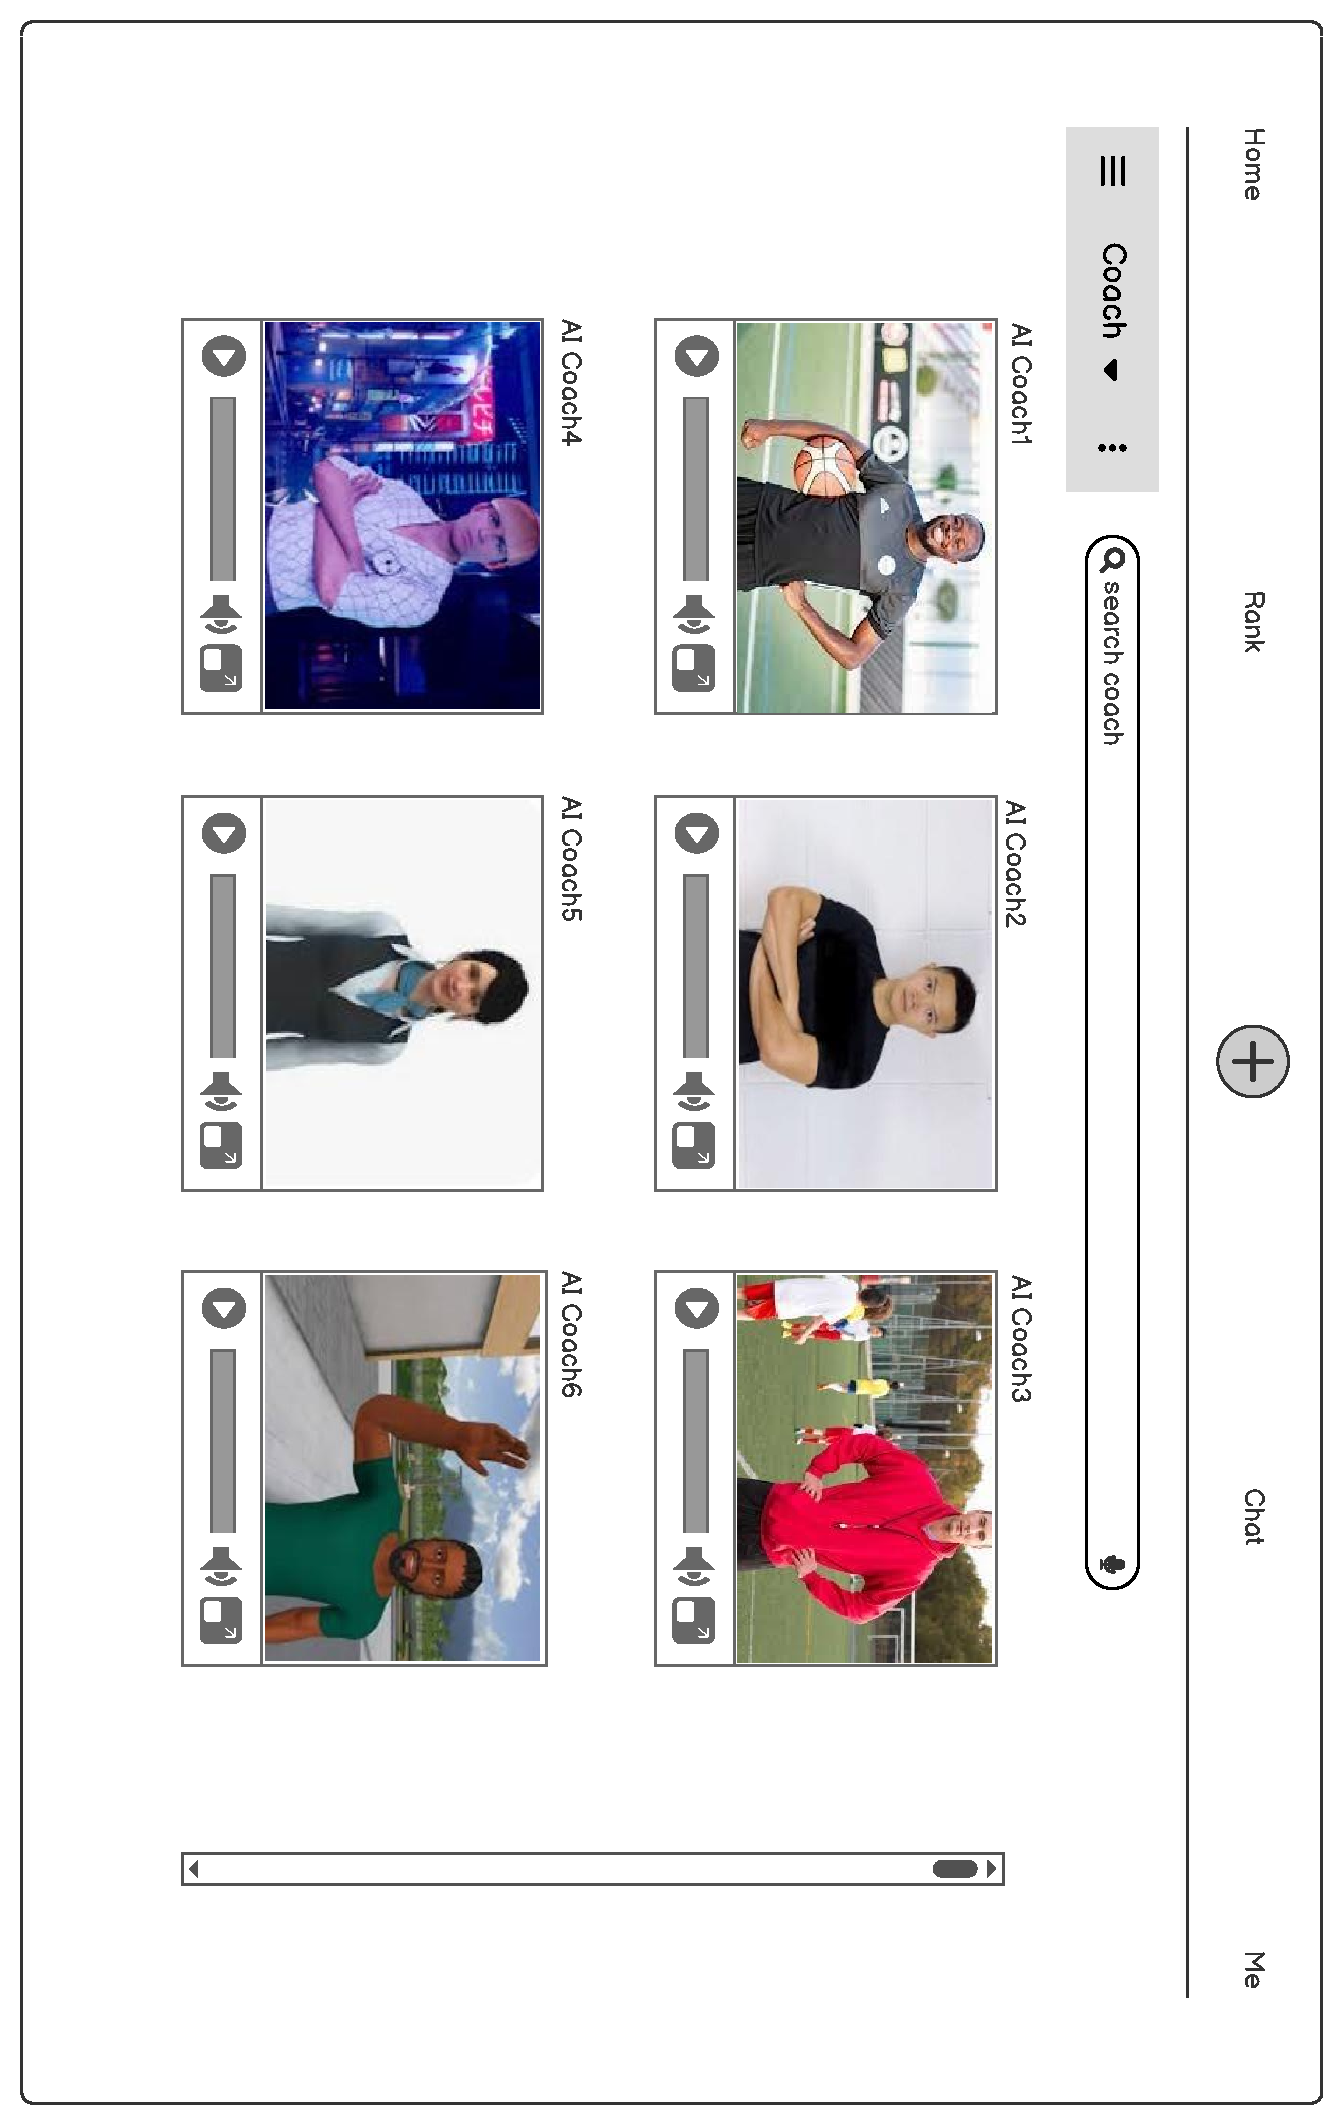
\includegraphics[width=1\textwidth]{images/UI_Final/UI_Final_3.pdf}
		\label{UI_3}
	\end{figure}

	\begin{figure}[H]
		\centering
		\caption*{\textbf{Diagram5.4} UI- Rank}
		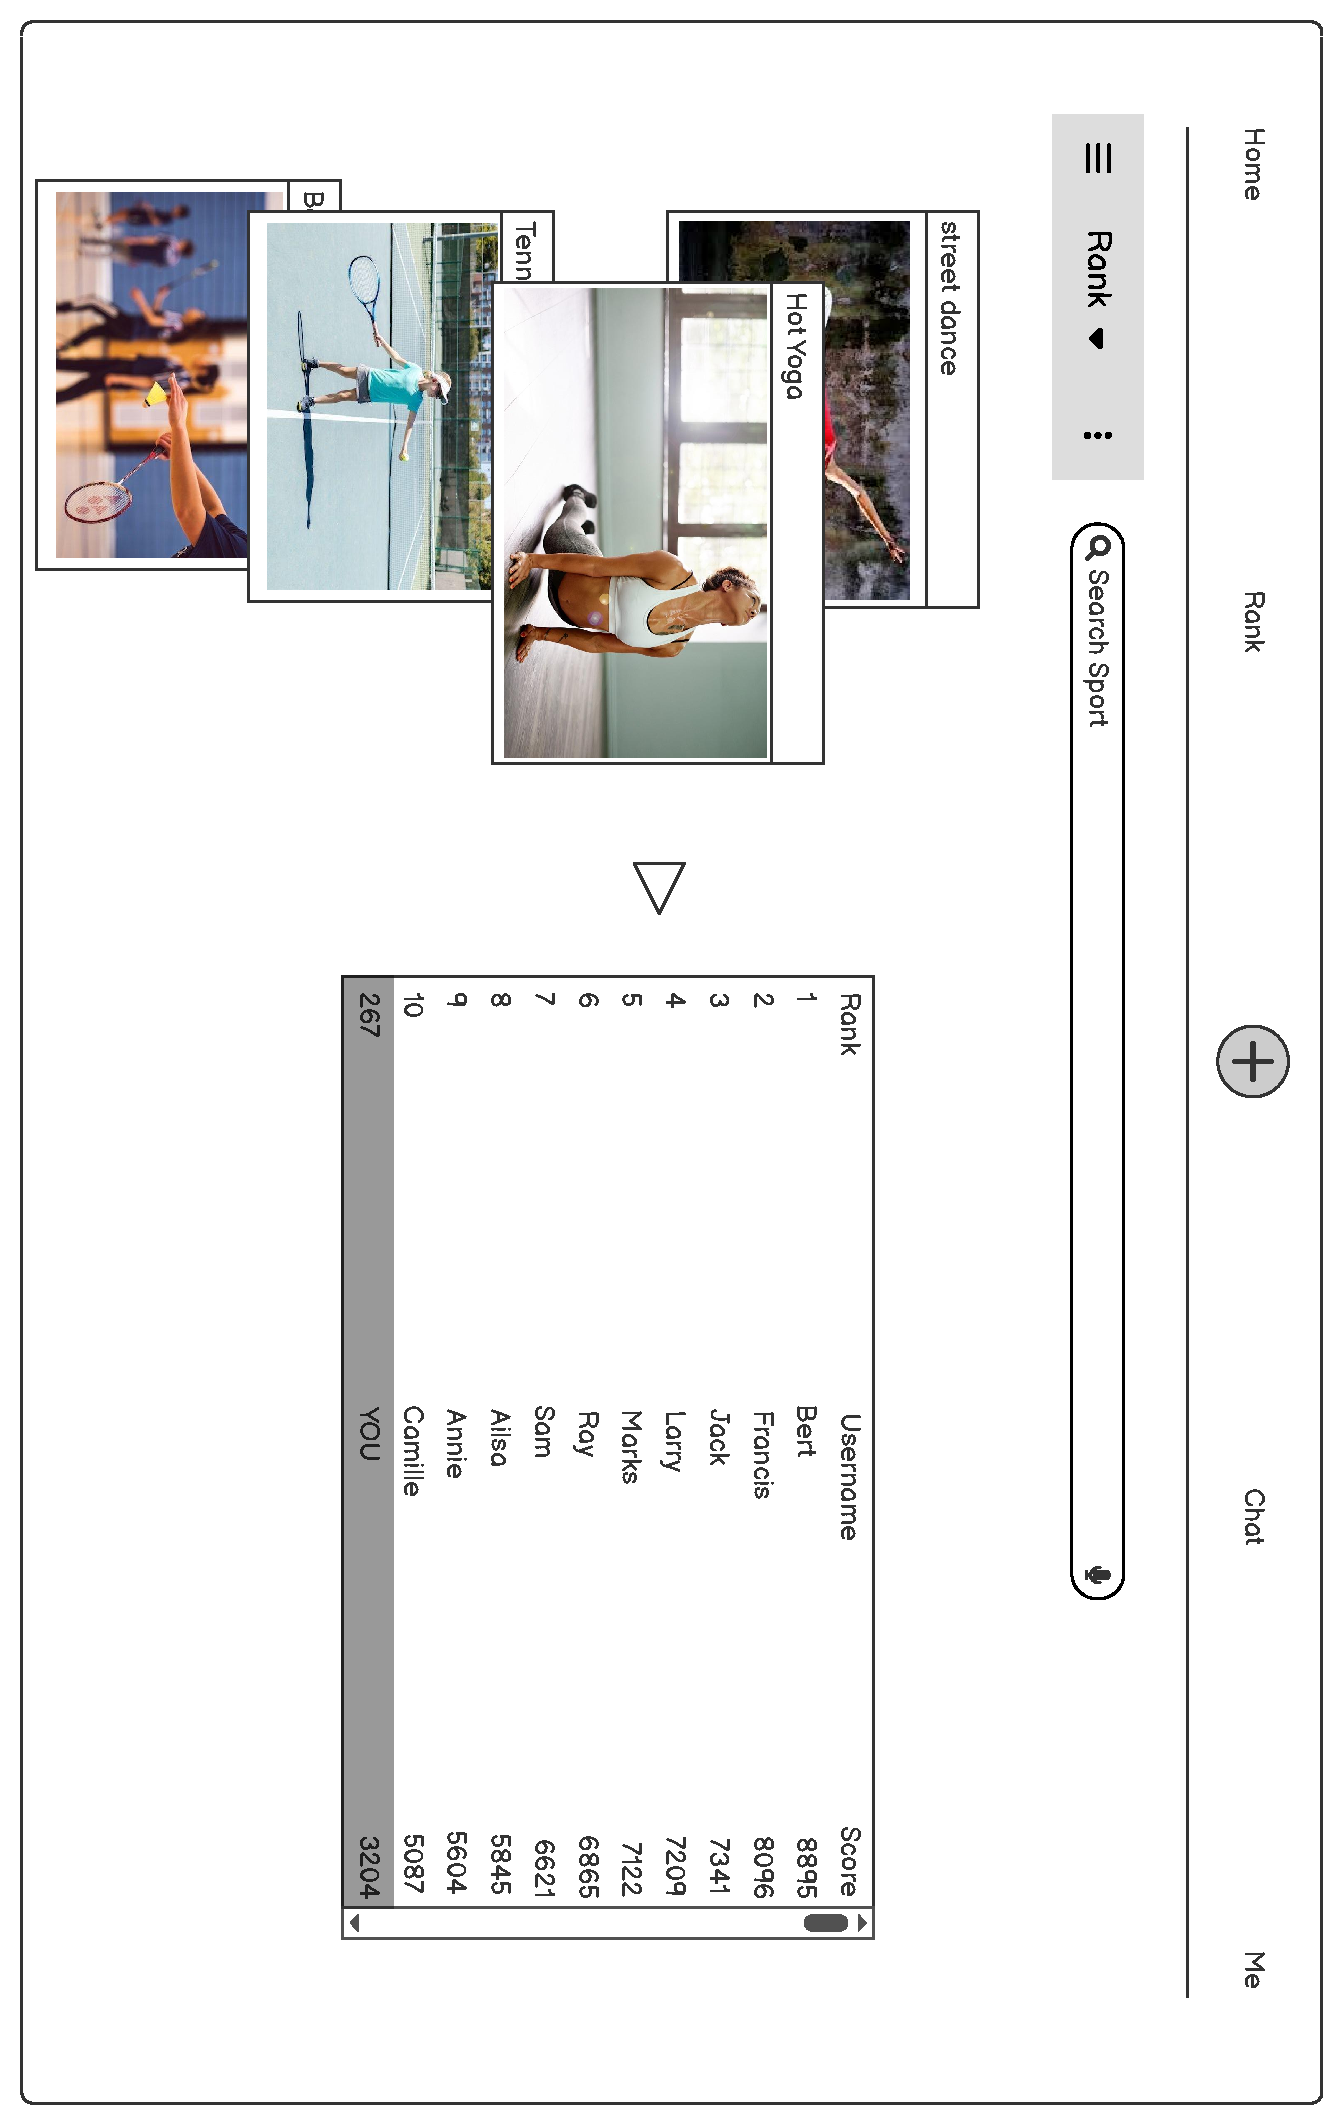
\includegraphics[width=1\textwidth]{images/UI_Final/UI_Final_4.pdf}
		\label{UI_4}
	\end{figure}

	\begin{figure}[H]
		\centering
		\caption*{\textbf{Diagram5.5} UI- Add friend}
		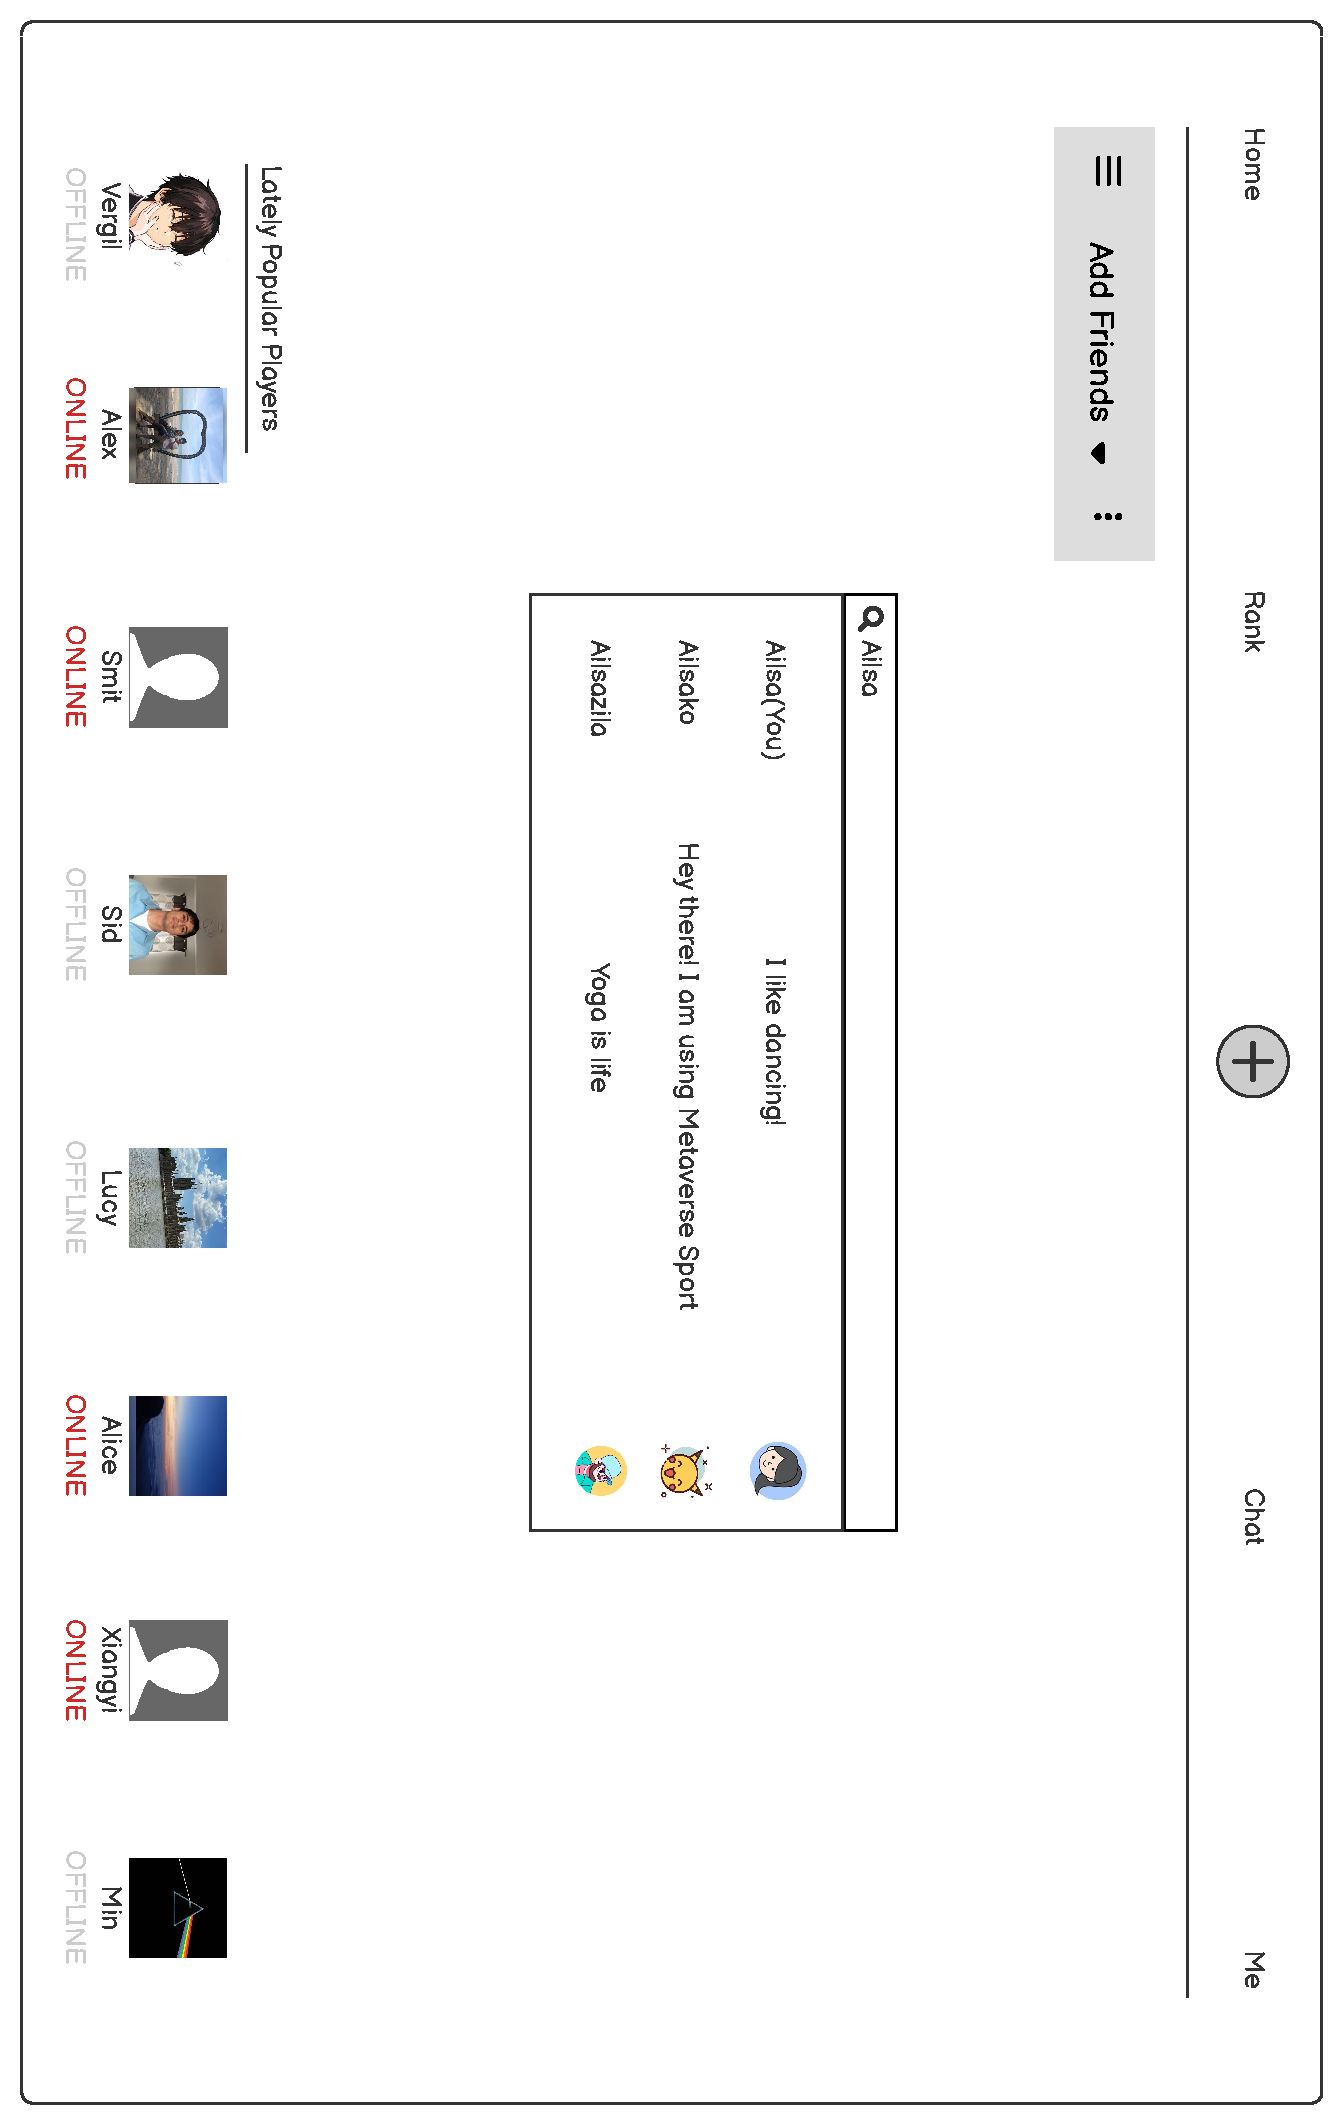
\includegraphics[width=1\textwidth]{images/UI_Final/UI_Final_5.pdf}
		\label{UI_5}
	\end{figure}

	\begin{figure}[H]
		\centering
		\caption*{\textbf{Diagram5.6} UI- Chat}
		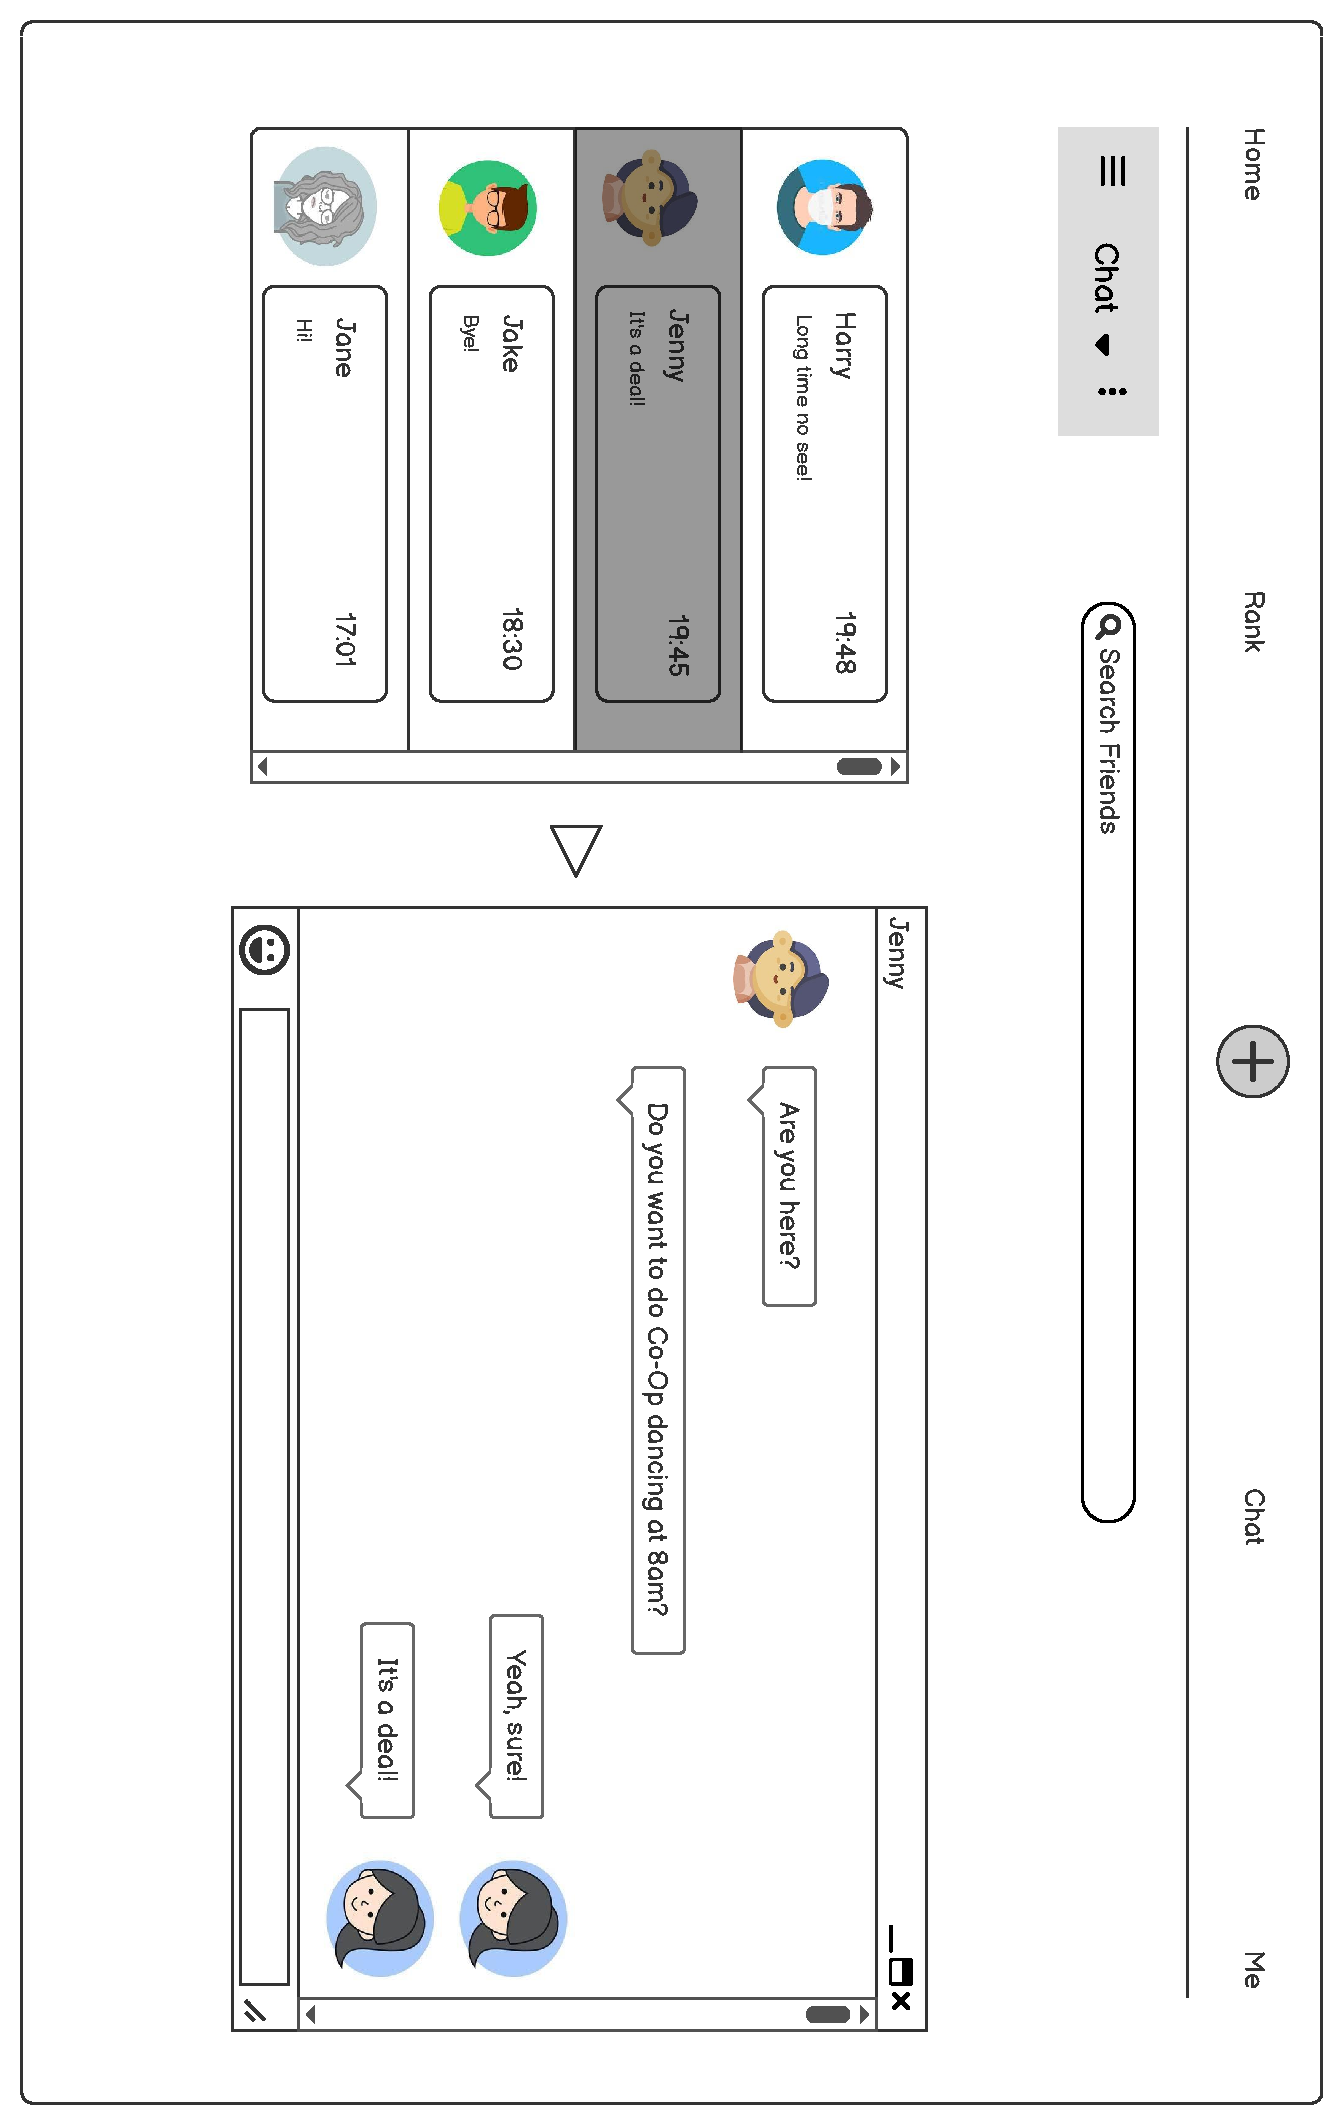
\includegraphics[width=1\textwidth]{images/UI_Final/UI_Final_6.pdf}
		\label{UI_6}
	\end{figure}

	\begin{figure}[H]
		\centering
		\caption*{\textbf{Diagram5.7} UI- Me}
		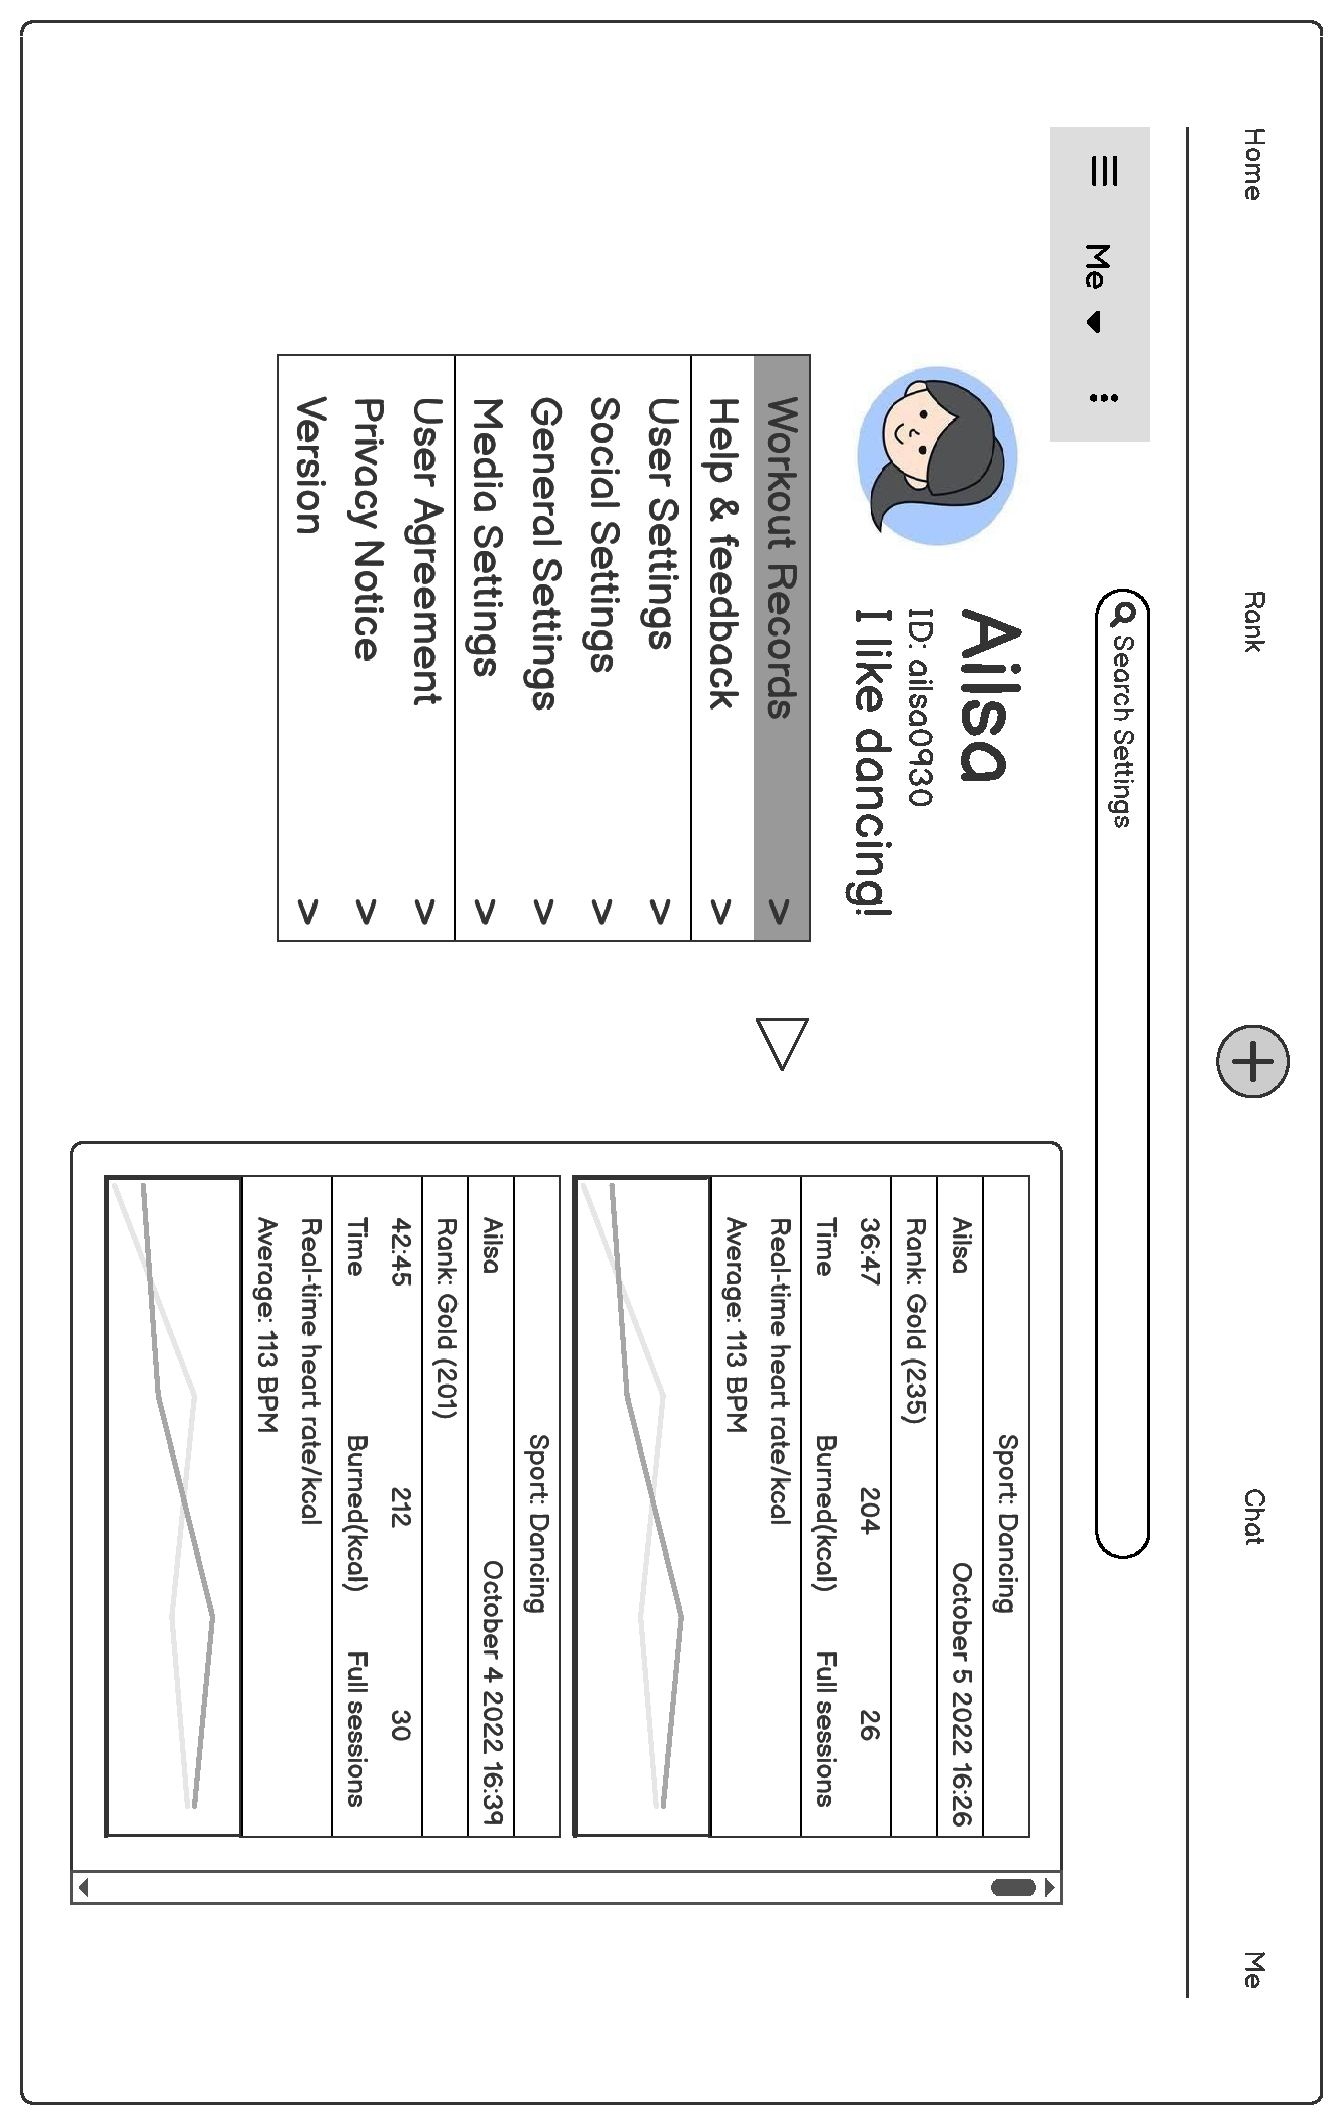
\includegraphics[width=1\textwidth]{images/UI_Final/UI_Final_7.pdf}
		\label{UI_7}
	\end{figure}
	\newpage

	%\subsection{Video Recording}

	\section{Ethics and Professional Practice}

	\noindent{\large{\textbf{Privacy and Confidentiality}}}\par
	The Metaverse Sport application collects and monitors the users' personal information including their health and sports performances. The collection and monitoring of the respective data should be strictly confidential and honour the users' privacy as stated in the ACM Code of Ethics (1.6 \& 1.7)\cite{ref5}. This means the users should be clearly informed of the type of personal information that will be gathered, the specific purposes for which the data will be used, the periods of data retention and disposal, rights to access and withdraw their consent for the data to be collected at any time including the rights to delete their existing data stored in the system. In addition, data handling should not violate the rights of the users by taking precautions to preserve their anonymity, ensure the accuracy of data, and protect it from unauthorised access for illegitimate purposes that are outside of the best interests of the stakeholders and accidental disclosures which will consequently lead to harms.
	
	\noindent{\large{\textbf{Fair and Non-Discriminatory}}}\par
	The Metaverse Sport application allows users to learn and practice sports with the help of motion detection and an AI coach including suggestions on specific movements and techniques based on data collected from professional athletes. The system further acknowledges that `standards' in human movements for playing sports should be initially set up to teach users, which may introduce bias and stereotyping. Following the ACM Code of Ethics (1.4)\cite{ref5}, the system needs to ensure fairness and avoid prejudicial discrimination by taking into consideration individuals of different ages, disability statuses, and cultural groups, as well as by continually revising and updating its design throughout time through improved data collection and modelling in order to minimize the possible bias associated with the enforcement of the `standardised' techniques onto different users. Besides that, since the system allows the engagement of multi-players when participating in sports online, it should clearly communicate to users that it will not tolerate harassment of any kind, including sexual harassment or bullying behaviour. Should in any event the users violate this policy, their access to engaging with the online community or multi-player will be terminated.

	\noindent{\large{\textbf{Honesty and Trustworthy}}}\par
	The ACM Code of Ethics (1.3)\cite{ref5} outlines honesty and trustworthiness as essential components of a system. Therefore, the Metaverse Sport application recognizes its limitations that it cannot replace real physical sports exercise or experience such as the feeling of the ball's inertia at impact when playing tennis or certain kinds of dancing which require a degree of physical contact i.e., salsa. Therefore, these should be communicated clearly to the stakeholders as the application intends to provide users with the closest experience to real-life sports and improve their cognitive performance.

	\noindent{\large{\textbf{Maintain the robustness of the system security}}}\par
	Since the system handles sensitive data, computing professionals should perform due diligence in the system design to ensure it functions as intended, and take appropriate action to prevent data breaches as clearly stated in the ACM Code of Ethics (2.9)\cite{ref5}. In cases where data breaches have occurred, notification should be given to affected parties in a timely and clear manner together with relevant guidance and remediation. 
	
	\newpage
	\section{Project Management and Moderation}

	%\noindent{\large{\textbf{Introduction}}}\par
	In order to meet the deadline, group7 holds two meetings a week, one is offline meeting discussing and assigning tasks for group members and one is a feedback session with Mr. Harry online. We assign the whole mission to 6 weeks' tasks and complete the corresponding tasks every week. In Total we had 5 feedback sessions and got lots of good advice. Every member participated in all of the meetings. Fortunately, we finished all of the tasks from week 5 to week 10 with perfect cooperation.\\

	\noindent{\large{\textbf{MinCheng Wu}}, 2458683, mxc1117@student.bham.ac.uk}\par
	I have attended all weekly meetings and completed tasks that have been distributed equally among us. My tasks have included describing the proposed system, Flow of Events, Object Diagrams, Testing Plan, and video recording together with the other team members. In addition, I was mainly responsible for identifying any code of ethics and professional practices that were relevant to the proposed system design and documenting this in the project report.\\
	
	\noindent{\large{\textbf{Minyueshen Chen}, 2401069, mxc1086@student.bham.ac.uk}}\par
	In the whole process of group work, I attended every group meeting with members and discussed with them. I mainly participated in the following parts of our group work: Functional requirements, Use case of `Edit personal information' (precondition, flow of events, postcondition and scenario 2), Object Diagram, Testing plan.\\

	\noindent{\large{\textbf{Saeed-Ul Haque}}, 2537125, sxh1515@student.bham.ac.uk}\par
	As an active team member, I helped refine and edit ideas and drafts to allow more understanding for the readers. I also brainstormed ideas with the group, aiding in creativity and rationality.  I worked cohesively in teams, where we were able to produce the following documents in collaboration: Requirements Engineering Introduction, Flow of Events: Doing Sports \& AI Coach, and Class Analysis; I have also been able to exhibit my independent work when creating the Architecture Analysis alone.\\

	\noindent{\large{\textbf{Smit Navinkumar}}, 2327596, sxn197@student.bham.ac.uk}\par
	I attended all of the group meetings and discussed the tasks with the group members. Every week, we split the tasks between the members fairly, and the ones I mainly participated in were: Functional requirements, Use case of `Register' (precondition, flow of events, post condition and the second scenario), Sequence diagram, Testing plan and the video recording.\\

	\noindent{\large{\textbf{WeiJu Chen}}, 2354176, wxc276@student.bham.ac.uk}\par
	At the first meeting, I suggested that the project should use the concept of Metaverse to learn new sports, and explained how to implement it in detail. After that I attended every group meeting, discussed with other members and gave suggestions to improve our project. Besides, I took part in the introduction, acting as an AI coach in the video recording. The content that I was responsible for are use case specification and scenarios, machine diagram, deployment diagram in the weekly group work.\\
	
	\noindent{\large{\textbf{Weilu Ma}}, 2411644, wxm145@student.bham.ac.uk}\par
	As a deputy, I booked the meeting room one time every week in the library and hosted the meeting as well as explained tasks in detail, then allocated the tasks to group members. Also, I took part in writing non-functional requirements in week5 and wrote one scenario of User Case in week6. I drew a Doing sports Sequence Diagram in week7 and Layered Style Deployment Diagram in week8. Besides, I drew a prime version of the interactive prototype then optimized it with partners in week9.\\

	\noindent{\large{\textbf{Xiangyi Zhou}}, 2416429, xxz234@student.bham.ac.uk}\par
	As a team member, I attended group discussion meetings and feedback sessions every week and worked in groups on time. The contexts I mainly participate in are including functional requirements, flow of events, state machine, testing plan and interactive prototype. In addition, I wrote a demonstration program of the interactive part as a reference for video recording.\\

	\noindent{\large{\textbf{Zijun Li}, 2272583, zxl183@student.bham.ac.uk}}\par
	I am the Scrum Master of our team. I am mainly responsible for the assignment of tasks, work inspection, collection, and optimization of each tasks, scheduling weekly feedback sessions and typesetting the final documents using Latex. The contents I participate in include: Non-functional requirement, flow of events and Scenarios for doing sport and adding friends, the activity diagrams of reporting a suspicious user, Class analysis, interactive prototype, and video recording. The prototypes I am responsible for are: use case diagram and components diagrams.

	\section{Reference}

	{\small\begingroup 
	\renewcommand{\section}[2]{}
	\begin{thebibliography}{99}

		\bibitem{ref1} Akmel, F., Birihanu, E., Siraj, B. and Shifaw, S. (2017) A Comparative Analysis on Software Architecture Styles. International Journal in Foundations of Computer Science \& Technology [online]. 7, pp. 11-22. [Accessed 24 Novemver 2022].
		\bibitem{ref2} Jaiswal, M. (2019) Software Architecture and Software Design. Social Science Research Network [online]. 6 (11) [Accessed 22 November 2022].
		\bibitem{ref3} Qureshi, N., Ikram, N., Bano, M. and Usman, M. (2011) Empirical Evidence in Software Architecture: A Systematic Literature Review Protocol. The Sixth International Conference on Software Engineering Advances [online]. [Accessed 22 November 2022].
		\bibitem{ref4} Wu, Y.S., Wang, Y.U., Chan, T.C., Lin, H.C., Chang, Y.T., Wu, H.Y., Liu, T.C., Chuang, Y.C., Wu, J., Chang, W.Y., Sun, C.A., Lin, M.C., Tseng, V.S., Hu, J.M., Li, Y.K., Hsiao, P.J., Chen, C.W., Kao, H.Y., Lee, C.C., Hsieh, C.B., Wang, C.H. and Chu, C.M. (2022) Effect of the Nintendo Ring Fit Adventure Exergame on Running Completion Time and Psychological Factors Among University Students Engaging in Distance Learning During the Covid-19 Pandemic: Randomized Controlled Trial. Jmir Serious Games [online]. 10 (0) [Accessed 31 October 2022].
		\bibitem{ref5} Acm.org. 2018. ACM Code of Ethics and Professional Conduct. [online] Available at: \url{http://www.acm.org/about-acm/acm-code-of-ethics-and-professional-conduct} [Accessed 24 November 2022].

	\end{thebibliography}
	\endgroup}

\end{document}
